\documentclass[11pt, a4paper]{article}
\usepackage[utf8]{inputenc}
\usepackage{amsmath, amssymb, amsthm}
\usepackage{geometry}
\usepackage{graphicx}
\usepackage{tikz-cd}
\usepackage{verbatim}
\geometry{left=2.5cm, right=2.5cm, top=2.5cm, bottom=2.5cm}
\usepackage[pdfencoding=auto,colorlinks=true,linkcolor=black,citecolor=blue,urlcolor=blue]{hyperref}
\usepackage{bookmark}
\hypersetup{
    pdftitle={Riemannian Geometry},
    pdfauthor={cc},
    pdfkeywords={Riemannian, geometry, lecture notes},
    bookmarksopen=true,
    bookmarksnumbered=true
}

\title{Riemannian Geometry}
\author{Instructor: John Lott \\ Scribe: cc}

% Theorem/definition environments: unified styles and numbering by section
\theoremstyle{plain}
\newtheorem{theorem}{Theorem}[section]
\newtheorem{lemma}[theorem]{Lemma}
\newtheorem{proposition}[theorem]{Proposition}
\newtheorem{corollary}[theorem]{Corollary}

\theoremstyle{definition}
\newtheorem{definition}[theorem]{Definition}
\newtheorem{example}[theorem]{Example}
\newtheorem{exercise}[theorem]{Exercise}

\theoremstyle{remark}
\newtheorem{remark}[theorem]{Remark}
\date{}
\newcommand{\p}{\partial}

\DeclareMathOperator{\End}{End}
\DeclareMathOperator{\tr}{tr}
\DeclareMathOperator{\Id}{Id}
\DeclareMathOperator{\diam}{diam}
\DeclareMathOperator{\Ric}{Ric}
\DeclareMathOperator{\Isom}{Isom}
\DeclareMathOperator{\Hess}{Hess}
\DeclareMathOperator{\Vol}{Vol}
\DeclareMathOperator{\inj}{inj}

\begin{document}

\maketitle

\tableofcontents
\newpage
\section{Lecture 1 is omitted.}
\section{Lecture 2}

\section*{Tensor Fields and $C^\infty(M)$-Multilinear Maps}

\textbf{Setup:} Consider a tensor field $F \in \mathcal{T}^k_l M$. Let $\omega^1, \dots, \omega^k \in \Omega^1(M)$ be 1-forms and $X_1, \dots, X_l \in \mathfrak{X}(M)$ be vector fields.

We can define a map:
\[
\mathcal{F}: \underbrace{\Omega^1(M) \times \dots \times \Omega^1(M)}_{k} \times \underbrace{\mathfrak{X}(M) \times \dots \times \mathfrak{X}(M)}_{l} \to C^\infty(M)
\]
by the pointwise evaluation:
\[
\mathcal{F}(\omega^1, \dots, \omega^k, X_1, \dots, X_l)(p) = F(\omega^1(p), \dots, \omega^k(p), X_1(p), \dots, X_l(p))
\]
Clearly, $\mathcal{F}$ is $C^\infty(M)$-multilinear.

\begin{lemma}
Any $C^\infty(M)$-multilinear map $\mathcal{F}$ comes from a unique tensor field $F \in \mathcal{T}^k_l M$.
\end{lemma}

\begin{itemize}
    \item \textbf{Algebraic Result:} For finite-dimensional vector spaces, we have the isomorphism $(V \otimes \dots \otimes V)^* \cong V^* \otimes \dots \otimes V^*$. In the context of manifolds, this extends to the module level over $C^\infty(M)$.
\end{itemize}

\subsection{Flow of a Vector Field}

\begin{definition}
Let $X \in \mathfrak{X}(M)$ be a vector field. The \emph{flow} of $X$ is a collection of (local) diffeomorphisms $\{\Phi_t\}$ such that if $\gamma(t) = \Phi_t(p)$, then:
\[
\frac{d\gamma}{dt} = X(\gamma(t)), \quad \gamma(0) = p
\]
\end{definition}

\begin{definition}
$X$ is called \emph{complete} if the flow $\Phi_t(p)$ exists for all $p \in M$ and all $t \in \mathbb{R}$. In this case, $\{\Phi_t\}$ forms a 1-parameter group of diffeomorphisms: $\Phi_{s+t} = \Phi_s \circ \Phi_t$.
\end{definition}

\begin{proposition}
If $M$ is a compact manifold, then every vector field $X$ on $M$ is complete. 
\end{proposition}
\textit{(Note: From now on, we assume vector fields are complete for simplicity.)}

\subsection{The Lie Derivative}

\section*{Lie Derivative of Functions}
\begin{definition}
For $f \in C^\infty(M)$, the Lie derivative of $f$ along $X$ is:
\[
\mathcal{L}_X f = \left. \frac{d}{dt} \right|_{t=0} (\Phi_t^* f) = \left. \frac{d}{dt} \right|_{t=0} (f \circ \Phi_t) = Xf
\]
\end{definition}

\section*{Lie Derivative of Differential Forms}
\begin{definition}
For $\omega \in \Omega^k(M)$, the Lie derivative is:
\[
\mathcal{L}_X \omega = \left. \frac{d}{dt} \right|_{t=0} \Phi_t^* \omega
\]
\end{definition}

\begin{lemma}
The Lie derivative commutes with the exterior derivative: $\mathcal{L}_X (d\omega) = d(\mathcal{L}_X \omega)$.
\end{lemma}
\begin{proof}
Since the pull-back $\Phi_t^*$ commutes with $d$:
\[
\mathcal{L}_X (d\omega) = \left. \frac{d}{dt} \right|_{t=0} \Phi_t^*(d\omega) = \left. \frac{d}{dt} \right|_{t=0} d(\Phi_t^* \omega) = d \left( \left. \frac{d}{dt} \right|_{t=0} \Phi_t^* \omega \right) = d(\mathcal{L}_X \omega)
\]
\end{proof}

\section*{Interior Multiplication}
Define the operator $i_X: \Omega^k(M) \to \Omega^{k-1}(M)$ by:
\[
(i_X \omega)(X_1, \dots, X_{k-1}) = \omega(X, X_1, \dots, X_{k-1})
\]
$i_X$ is a graded derivation of degree $-1$:
\[
i_X(\omega \wedge \eta) = (i_X \omega) \wedge \eta + (-1)^{\deg \omega} \omega \wedge (i_X \eta)
\]

\subsection{Cartan's Magic Formula}

\begin{lemma}
The algebra $\Omega^*(M)$ is generated by $C^\infty(M)$ and $\{df \mid f \in C^\infty(M)\}$.
\end{lemma}
\begin{proof}
Choose a coordinate neighborhood $(U, x^i)$. Any $\omega \in \Omega^k(U)$ can be written as $\omega = \sum \omega_I dx^I$. Using a partition of unity $\sum \phi_i = 1$ subordinate to an atlas $\{U_i\}$, we can write any global form as a sum of such local terms.
\end{proof}

\begin{proposition}[Cartan's Magic Formula]
$\mathcal{L}_X = d i_X + i_X d$
\end{proposition}
\begin{proof}
Both $\mathcal{L}_X$ and $d i_X + i_X d$ are graded derivations of degree 0 on $\Omega^*(M)$. Thus, it suffices to check the identity on generators:
\begin{enumerate}
    \item \textbf{On functions $f \in C^\infty(M)$:}
    \[ (d i_X + i_X d)f = d(i_X f) + i_X(df) = 0 + df(X) = Xf = \mathcal{L}_X f \]
    \item \textbf{On exact 1-forms $df$:}
    \[ (d i_X + i_X d)df = d(i_X df) + i_X(d^2 f) = d(Xf) + 0 = d(\mathcal{L}_X f) = \mathcal{L}_X (df) \]
\end{enumerate}
Since the operators agree on generators and satisfy the same Leibniz rule, they are equal.
\end{proof}

\subsection{Lie Derivative of Vector Fields}

\begin{definition}
Let $Y \in \mathfrak{X}(M)$. Its Lie derivative along $X$ is defined as:
\[
\mathcal{L}_X Y = \left. \frac{d}{dt} \right|_{t=0} (\Phi_{-t})_* Y = \left. \frac{d}{dt} \right|_{t=0} (\Phi_t^* Y)
\]
\end{definition}

\begin{proposition}
Let $\omega$ be a 1-form and $X, Y$ be vector fields. Then:
\[
X(\omega(Y)) = (\mathcal{L}_X \omega)(Y) + \omega(\mathcal{L}_X Y)
\]
\end{proposition}
\begin{proof}
Evaluating at $p \in M$:
\begin{align*}
X(\omega(Y))_p &= \left. \frac{d}{dt} \right|_{t=0} (\omega(Y))(\Phi_t(p)) \\
&= \left. \frac{d}{dt} \right|_{t=0} \langle \Phi_t^* \omega, \Phi_t^* Y \rangle_p \\
&= \langle \left. \frac{d}{dt} \right|_{t=0} \Phi_t^* \omega, Y \rangle_p + \langle \omega, \left. \frac{d}{dt} \right|_{t=0} \Phi_t^* Y \rangle_p \\
&= (\mathcal{L}_X \omega)(Y) + \omega(\mathcal{L}_X Y)
\end{align*}
\end{proof}

\begin{proposition}
$\mathcal{L}_X Y = [X, Y]$, where $[X, Y]$ is the Lie bracket.
\end{proposition}
\begin{proof}
Let $f \in C^\infty(M)$ be a test function. Consider the 1-form $df$:
\begin{align*}
\langle df, \mathcal{L}_X Y \rangle &= X(df(Y)) - (\mathcal{L}_X df)(Y) \quad \text{(using the previous Prop)} \\
&= X(Yf) - d(Xf)(Y) \\
&= X(Yf) - Y(Xf) = [X, Y]f
\end{align*}
Since this holds for all $f$, $\mathcal{L}_X Y = [X, Y]$.
\end{proof}
\newpage
\section{Lecture 3}

\subsection{Riemannian Metric}

\begin{definition}
A \textbf{Riemannian metric} on a smooth manifold $M$ is a covariant tensor field $g$ of type $(0,2)$ which is symmetric and positive definite.
Specifically, for each $p \in M$, $g_p: T_p M \times T_p M \to \mathbb{R}$ satisfies:
\begin{enumerate}
    \item \textbf{Symmetry:} $g(X, Y) = g(Y, X)$ for all $X, Y \in \mathfrak{X}(M)$.
    \item \textbf{Positive Definiteness:} $g(X, X) \ge 0$, and $g(X, X) = 0 \iff X = 0$.
\end{enumerate}
\end{definition}
\textbf{Notation:} We often write $\langle X, Y \rangle = g(X, Y)$.

\begin{proposition}
Every smooth manifold $M$ admits a Riemannian metric.
\end{proposition}
\begin{proof}[Sketch of Proof]
Take an atlas $\{U_i\}$ of $M$. On each $U_i$, define a local metric $g_i = \sum (dx^k)^2$. Let $\{\phi_i\}$ be a partition of unity subordinate to $\{U_i\}$. Then $g = \sum \phi_i g_i$ is a well-defined global Riemannian metric because a convex combination of positive definite symmetric forms remains positive definite and symmetric.
\end{proof}

Suppose we are given a local coordinate $(U,\{x^1,...,x^n\})$, then we can expressed the metric locally as $g = g_{ij}dx^i dx^j$ since g is symmetric. 
Further, if $M$ has a local frame $\{E_1,...,E_n\}$ with coframe $\{\varepsilon^1,...,\varepsilon^n\}$, then $g = \sum g(E_i, E_j) \varepsilon^i \varepsilon^j$. 
We can consider the case where $\{E_i\}$ is orthonormal, in this case, $g = \sum (\varepsilon^i)^2$.

\begin{proposition}[Existence of Orthonormal Frame]
    If $\{X_j\}$ is a local frame on $(M, g)$, then there exists an orthonormal frame $\{E_i\}$ obtained from $\{X_j\}$ via the Gram-Schmidt process.
\end{proposition}

\subsection{Isometries}

\begin{definition}
Let $(M, g)$ and $(\tilde{M}, \tilde{g})$ be Riemannian manifolds.
\begin{enumerate}
    \item A diffeomorphism $\Phi: M \to \tilde{M}$ is an \textbf{isometry} if $g = \Phi^* \tilde{g}$, i.e.,
    \[ g_p(X, Y) = \tilde{g}_{\Phi(p)}(d\Phi_p(X), d\Phi_p(Y)) \quad \forall X, Y \in T_p M \]
    \item The set of all isometries from $(M, g)$ to itself forms the \textbf{Isometry Group}, denoted $\text{Isom}(M, g)$.
\end{enumerate}
\end{definition}

\subsection{Examples of Constructions}

\textbf{1. Induced Metric:} If $i: M \to \tilde{M}$ is an immersion and $\tilde{g}$ is a metric on $\tilde{M}$, then $g = i^* \tilde{g}$ is the induced Riemannian metric on $M$.

\noindent\textbf{2. Warped Product:} Given $(M_1, g_1), (M_2, g_2)$ and $f \in C^\infty(M_1, \mathbb{R}^+)$, the warped product $M_1 \times_f M_2$ has the metric:
\[ g = g_1 + f^2 g_2 \]
Formally: $g((X_1, Y_1), (X_2, Y_2)) = g_1(X_1, X_2) + f^2(p_1) g_2(Y_1, Y_2)$.

\begin{example}[Warped Product]
    Here are some examples of warped products:
    \begin{itemize}
        \item The polar coordinates on $\mathbb{R}^2 \setminus \{0\}$ can be viewed as a warped product $(0, \infty) \times_r S^1$ with metric $dr^2 + r^2 d\theta^2$.
        \item The sphere $S^n \setminus \{\text{north, south poles}\}$ can be represented as $(0, \pi) \times_{\sin r} S^{n-1}$ with metric $dr^2 + \sin^2(r) g_{S^{n-1}}$.
    \end{itemize}
\end{example}

\section*{Riemann Submanifolds}
\begin{lemma}
Let $i: M \to \tilde{M}$ be an embedding and $\tilde{g}$ a Riemannian metric on $\tilde{M}$. Then the induced metric $g = i^* \tilde{g}$ makes $(M, g)$ a Riemannian submanifold of $(\tilde{M}, \tilde{g})$.
\end{lemma}

\section*{Riemann Products}
Given two Riemannian manifolds $(M_1, g_1)$ and $(M_2, g_2)$, the product manifold $M_1 \times M_2$ has a natural Riemannian metric defined by:
\[ g((X_1, Y_1), (X_2, Y_2)) = g_1(X_1, X_2) + g_2(Y_1, Y_2) \]

\subsection{Vector Bundles and Distributions}

Let $E \to M$ be a vector bundle. An \textbf{inner product on $E$} is a smooth choice of inner product $\langle \cdot, \cdot \rangle$ on each fiber $E_m$. For any smooth sections $s_1, s_2 \in \Gamma(E)$, the function $m \mapsto \langle s_1(m), s_2(m) \rangle$ is in $C^\infty(M)$.

\textbf{Vertical and Horizontal Bundles:}
Let $\pi: \tilde{M} \to M$ be a submersion.
\begin{itemize}
    \item \textbf{Vertical Bundle:} $T^V \tilde{M} = \ker(d\pi)$.
    \item \textbf{Splitting:} A choice of \textbf{Horizontal Distribution} $T^H \tilde{M}$ such that $T\tilde{M} = T^V \tilde{M} \oplus T^H \tilde{M}$.
    \item \textbf{Riemannian Choice:} If $\tilde{M}$ has metric $\tilde{g}$, we naturally define $T^H \tilde{M} = (T^V \tilde{M})^\perp$.
\end{itemize}

\begin{proposition}
    Let $\pi:\tilde{M}\to M$ be smooth submersion of Riemannian manifolds. Then
    \begin{itemize}
        \item Every smooth vector field $W$ on $\tilde{M}$ can be uniquely decomposed as $W = W^V + W^H$ with $W^V \in T^V \tilde{M}$ and $W^H \in T^H \tilde{M}$.
        \item For any smooth vector field $X$ on $M$, there exists a unique horizontal lift $\tilde{X}$ on $\tilde{M}$ such that $d\pi(\tilde{X}) = X$. 
    \end{itemize}
\end{proposition}

\subsection{Riemannian Submersion}

\begin{definition}
A submersion $\pi: (\tilde{M}, \tilde{g}) \to (M, g)$ is a \textbf{Riemannian submersion} if for all $\tilde{p} \in \tilde{M}$, the map $d\pi_{\tilde{p}}$ restricted to the horizontal space is a linear isometry:
\[ d\pi_{\tilde{p}}: (T^H_{\tilde{p}} \tilde{M}, \tilde{g}) \xrightarrow{\cong} (T_{\pi(\tilde{p})} M, g) \]
\end{definition}

Recall that we say a group acts \textbf{freely} on X if $gX = X$ implies $g = e$. We say the action is \textbf{proper} if the map $G \times \tilde{M} \to \tilde{M} \times \tilde{M}$, $(g, p) \mapsto (gp, p)$ is a proper map (i.e. the preimage of any compact set is compact).

\begin{proposition}
Let $G$ be a Lie group acting freely and properly on $(\tilde{M}, \tilde{g})$ by isometries. Then the quotient $M = \tilde{M}/G$ is a smooth manifold and admits a unique Riemannian metric $g$ such that the projection $\pi: \tilde{M} \to M$ is a Riemannian submersion.
\end{proposition}

\begin{proof}
    First, what is $\tilde{M}/G$? This is the set of orbits and the topology is the quotient topology. We define the Riemann metric on
    $M$ as follows: For $p \in M$, choose representative $\tilde{p} \in \tilde{M}$ with $\pi(\tilde{p}) = p$. For vectors $u,\,v \in T_p M$, define
    \[ g(u, v) = \tilde{g}(\tilde{u}, \tilde{v})\quad \tilde{u},\,\tilde{v} \in T_{\tilde{p}}^H \tilde{M}\text{ so that } d\pi_{\tilde{p}}(\tilde{u}) = u \text{ and } d\pi_{\tilde{p}}(\tilde{v}) = v. \]
    We have to check this is well-defined. If we choose another representative $\tilde{p}' = g\tilde{p}$ for some $g \in G$, then since $G$ acts by isometries, we have 
    \[ \tilde{g}((dg)_{\tilde{p}}(\tilde{u}), (dg)_{\tilde{p}}(\tilde{v})) = \tilde{g}(\tilde{u}, \tilde{v}). \]
    Also, since $\pi \circ g = \pi$, we have $(dg)_{\tilde{p}}$ maps horizontal spaces to horizontal spaces because it is an isometry. Thus the definition of $g$ is independent of the choice of representative.

    Finally, smoothness of $g$ follows from the smoothness of $\tilde{g}$ and the local triviality of the bundle structure induced by the free and proper action.
\end{proof}

\subsection{Riemann Covering Spaces}

\begin{definition}
Let $\pi: \tilde{M} \to M$ be a smooth map. We say $\pi$ is a \textbf{covering map} if for every $m \in M$, there exists an open neighborhood $U \subset M$ of $m$ such that:
\[
\pi^{-1}(U) = \coprod_{i} V_i
\]
where each $V_i \subset \tilde{M}$ is an open set, and the restriction $\pi|_{V_i}: V_i \to U$ is a \textbf{diffeomorphism} for every $i$.
\end{definition}

\section*{Metrics on Covering Spaces}

If $g$ is a Riemannian metric on the base manifold $M$, we can naturally obtain a Riemannian metric $\tilde{g}$ on the covering space $\tilde{M}$ via the pullback map:
\[
\tilde{g} = \pi^* g
\]
Since $\pi$ is a local diffeomorphism, $\tilde{g}$ is a well-defined Riemannian metric on $\tilde{M}$, making $\pi$ a local isometry.

\section*{*Normal Coverings and Descent of Metrics}

Now consider the inverse problem: given a Riemannian metric $\tilde{g}$ on $\tilde{M}$, when does it descend to a metric $g$ on $M$ such that $\pi^* g = \tilde{g}$?

\begin{definition}
$\pi: \tilde{M} \to M$ is a \textbf{normal (or Galois) covering} if the fundamental group $\pi_1(\tilde{M})$ is a normal subgroup of $\pi_1(M)$. In this case, the group of Deck transformations is:
\[
G = \text{Deck}(\tilde{M}/M) \cong \pi_1(M) / \pi_1(\tilde{M})
\]
\end{definition}

\begin{proposition}
Suppose $\pi: \tilde{M} \to M$ is a normal covering and $\tilde{g}$ is a Riemannian metric on $\tilde{M}$. There exists a unique Riemannian metric $g$ on $M$ such that $\pi^* g = \tilde{g}$ if and only if the group $G$ acts on $(\tilde{M}, \tilde{g})$ by \textbf{isometries}.
\end{proposition}

\newpage

\section{Lecture 4}

\subsection{Raising and Lowering Indices (Musical Isomorphisms)}

The Riemannian metric $g$ provides a natural isomorphism between the tangent bundle $TM$ and the cotangent bundle $T^*M$.

\section*{Lowering Indices (The Flat Operator $\flat$)}
Let $X \in T_p M$. We define $X^\flat \in T_p^* M$ by:
\[ X^\flat(Y) = \langle X, Y \rangle_g = g(X, Y) \]
In local coordinates, if $X = X^j \partial_j$, then:
\[ X^\flat(\partial_i) = g(\partial_j, \partial_i) X^j = g_{ij} X^j \]
Thus, the component expression is:
\[ X^\flat = (g_{ij} X^j) dx^i = X_i dx^i \]

\section*{Raising Indices (The Sharp Operator $\sharp$)}
Let $\omega \in T_p^* M$. We define $\omega^\sharp \in T_p M$ by the condition:
\[ \langle \omega^\sharp, X \rangle_g = \omega(X) \quad \forall X \in T_p M \]
In local coordinates, if $\omega = \omega_i dx^i$, then:
\[ \omega^\sharp = (g^{ij} \omega_i) \partial_j = \omega^j \partial_j \]
where $(g^{ij})$ is the inverse matrix of $(g_{ij})$, i.e., $g^{ij} g_{jk} = \delta^i_k$.

\section*{Examples}
\begin{enumerate}
    \item \textbf{Gradient:} For $f \in C^\infty(M)$, the differential $df = \partial_i f dx^i$ is a 1-form. Its "sharp" version is the gradient vector field:
    \[ \text{grad} f = (df)^\sharp = g^{ij} \partial_i f \partial_j \]
    \item \textbf{Inner Product of 1-forms:} Let $\omega, \eta \in \Omega^1(M)$. Their inner product is defined via the isomorphism:
    \[ \langle \omega, \eta \rangle_g = \langle \omega^\sharp, \eta^\sharp \rangle_g = g^{ij} \omega_i \eta_j \]
\end{enumerate}

\subsection{Volume Form and Density}

Let $(M, g)$ be an oriented Riemannian manifold of dimension $n$.

\begin{definition}
The \textbf{Riemannian volume form} $dV$ is the unique $n$-form such that for any oriented orthonormal basis $\{E_1, \dots, E_n\}$ of $T_p M$, we have:
\[ dV(E_1, \dots, E_n) = 1 \]
\end{definition}

\begin{proposition}
In local coordinates $(x^1, \dots, x^n)$, the volume form is expressed as:
\[ dV = \sqrt{\det(g_{ij})} \, dx^1 \wedge \dots \wedge dx^n \]
The corresponding measure for integration is often denoted as the \textbf{Riemannian density}:
\[ d\mu = \sqrt{\det g} \, d^n x \]
\end{proposition}

\subsection{Length and Distance}

Let $\gamma: [a, b] \to M$ be a smooth curve.
\begin{itemize}
    \item \textbf{Length:} The length of $\gamma$ is defined as:
    \[ L(\gamma) = \int_a^b |\dot{\gamma}(t)|_g \, dt = \int_a^b \sqrt{g(\dot{\gamma}(t), \dot{\gamma}(t))} \, dt \]
    \item \textbf{Invariance:} Length is invariant under reparametrization.
    \item \textbf{Regularity:} $\gamma$ is \textit{regular} if $\dot{\gamma}(t) \neq 0$ for all $t$ (i.e., it is an immersion). $\gamma$ is \textit{admissible} if it is continuous and piecewise regular.
    \item \textbf{Arc-length Parameter:} $s(t) = \int_a^t |\dot{\gamma}(u)| du$. Under this reparametrization, $|\frac{d\gamma}{ds}| = 1$ (unit speed).
\end{itemize}

\begin{proposition}
If $(M,g) \to (\tilde{M}, \tilde{g})$ is an isometry, then the induced map preserves lengths. i.e. $L(\gamma) = L(\Phi \circ \gamma)$.
\end{proposition}

\textbf{Distance Definition:} For a connected Riemannian manifold $(M, g)$, the distance $d(p, q)$ between $p, q \in M$ is defined as:
\[ d(p, q) = \inf \{ L(\gamma) \mid \gamma: [a, b] \to M \text{ is admissible, } \gamma(a)=p, \gamma(b)=q \} \]
This definition exists since the manifold is connected and the path is compact.

\begin{theorem}
     $(M, d)$ is a metric space, and the metric topology coincides with the manifold topology.
\end{theorem}
The key step is to show that in local coordinates, the Riemannian metric is equivalent to the Euclidean metric.
\begin{lemma}
    Let $(M,g)$ be Riemannian manifold and $(U,\{x^1,...,x^n\})$ be a local coordinate system. Set $\bar{g}$ be the Euclidean metric
    on $U$ defined by $\bar{g}=\sum (dx^i)^2$. Then for any compact set $K\subset U$, and $x\in K$, $v\in T_x M$, we have
    \[ |v|_{\bar{g}} \approx_{C_k} |v|_g. \]
\end{lemma}
\begin{proof}
    Consider the continuous function $F: TU \to \mathbb{R}$ by $F(x,v) |v|_g$. Since $K$ is compact, $F$ attains a minimum and maximum on the set $\{(x,v)\in TU| x\in K, |v|_{\bar{g}}=1\}$. 
\end{proof}

\subsection{Maximally Symmetric Spaces}

\section*{Definitions}
\begin{itemize}
    \item \textbf{Homogeneous:} The isometry group $\text{Isom}(M, g)$ acts transitively on $M$.
    \item \textbf{Isotropic:} The isometry group $\text{Isom}(M, g)$ acts transitively on the unit tangent bundle $T^1 M$. Recall the action is given by $d\Phi_p(v)$ for $\Phi \in \text{Isom}(M, g)$, $p \in M$, and $v \in T_p^1 M$.
    \item \textbf{Frame Isotropic:} $\text{Isom}(M, g)$ acts transitively on the bundle of orthonormal frames $O(M)$. This implies $M$ has constant sectional curvature.
\end{itemize}

\subsection{Examples of Riemannian Manifolds with Maximal Symmetry}
\begin{enumerate}
    \item \textbf{Euclidean Space $\mathbb{R}^n$:} Standard metric $g = \sum (dx^i)^2$. $\text{Isom}(\mathbb{R}^n) = \mathbb{R}^n \rtimes O(n)$. $\dim = n + \frac{n(n-1)}{2} = \frac{n(n+1)}{2}$.
    \item \textbf{Sphere $S^n$:} Metric induced from $\mathbb{R}^{n+1}$. $\text{Isom}(S^n) = O(n+1)$. $\dim = \frac{n(n+1)}{2}$.
    \item \textbf{Hyperbolic Space $\mathbb{H}^n$:} Constant curvature $K = -1$.
    \begin{itemize}
        \item \textbf{Hyperboloid Model:} In $\mathbb{R}^{n,1}$, surface $\tau^2 - \sum (\xi^i)^2 = 1, \tau > 0$.
        \item \textbf{Poincaré Ball Model:} $B^n = \{x \in \mathbb{R}^n \mid |x| < 1\}$, $g = \frac{4 \sum (dx^i)^2}{(1-|x|^2)^2}$.
        \item \textbf{Upper Half-Plane Model:} $U^n = \{(x_1, \dots, y) \in \mathbb{R}^n \mid y > 0\}$, $g = \frac{\sum (dx^i)^2 + dy^2}{y^2}$.
    \end{itemize}
    $\text{Isom}(\mathbb{H}^n) \cong O(n, 1)$. $\dim = \frac{n(n+1)}{2}$.
\end{enumerate}
\newpage
\section{Lecture 5}

\subsection{Three Models of Hyperbolic Space $\mathbb{H}^n$}

Hyperbolic space can be represented by several isometric models. We focus on the Upper Half-Plane model ($\mathbb{U}^n$), the Poincaré Ball model ($\mathbb{B}^n$), and the Hyperboloid model.

\subsection*{Metrics and Transformations}

\begin{itemize}
    \item \textbf{Upper Half-Plane Model $\mathbb{U}^n$}: 
    Defined on $\{ (x_1, \dots, y) \in \mathbb{R}^n : y > 0 \}$. In dimension 2 ($z = x + iy$):
    \[ g_{\mathbb{U}} = \frac{dx^2 + dy^2}{y^2} = \frac{dz d\bar{z}}{(\text{Im}\, z)^2} \]
    
    \item \textbf{Poincaré Ball Model $\mathbb{B}^n$}: 
    Defined on $\{ w \in \mathbb{R}^n : |w| < 1 \}$. In dimension 2 ($w = u + iv$):
    \[ g_{\mathbb{B}} = 4 \frac{du^2 + dv^2}{(1 - |w|^2)^2} = 4 \frac{dw d\bar{w}}{(1 - |w|^2)^2} \]
\end{itemize}

\textbf{Cayley Transform:} The isometry $X: \mathbb{B}^2 \to \mathbb{U}^2$ is given by the Möbius transformation:
\[ z = X(w) = -i \frac{w + i}{w - i} \]

\begin{proof}[Verification of Isometry]
1. Compute the differential $dz$:
\[ dz = -i \frac{(w-i) - (w+i)}{(w-i)^2} dw = -i \frac{-2i}{(w-i)^2} dw = \frac{-2}{(w-i)^2} dw \]
Thus, $dz d\bar{z} = \frac{4}{|w-i|^4} dw d\bar{w}$.

2. Compute the imaginary part $\text{Im}\, z$:
\[ \text{Im}\, z = \frac{1}{2i} (z - \bar{z}) = \frac{1}{2i} \left( -i \frac{w+i}{w-i} - i \frac{\bar{w}-i}{\bar{w}+i} \right) = - \frac{1}{2} \left( \frac{(w+i)(\bar{w}+i) + (\bar{w}-i)(w-i)}{|w-i|^2} \right) \]
\[ \text{Im}\, z = - \frac{1}{2} \left( \frac{(w\bar{w} + iw + i\bar{w} - 1) + (w\bar{w} - iw - i\bar{w} - 1)}{|w-i|^2} \right) = \frac{1 - |w|^2}{|w-i|^2} \]

3. Substitute into the metric $g_{\mathbb{U}}$:
\[ \frac{dz d\bar{z}}{(\text{Im}\, z)^2} = \frac{4 / |w-i|^4}{(1-|w|^2)^2 / |w-i|^4} dw d\bar{w} = \frac{4 dw d\bar{w}}{(1-|w|^2)^2} = g_{\mathbb{B}} \]
\end{proof}

\subsection{Isometry Groups}

The groups of orientation-preserving isometries for these models are isomorphic:
\begin{itemize}
    \item $\text{Isom}^+(\mathbb{U}^2) \cong PSL(2, \mathbb{R}) = \{ \begin{pmatrix} a & b \\ c & d \end{pmatrix} : a,b,c,d \in \mathbb{R}, ad-bc=1 \} / \{\pm I\}$.
    \item $\text{Isom}^+(\mathbb{B}^2) \cong PSU(1, 1) = \{ \begin{pmatrix} \alpha & \beta \\ \bar{\beta} & \bar{\alpha} \end{pmatrix} : |\alpha|^2 - |\beta|^2 = 1 \} / \{\pm I\}$.
    \item $\text{Isom}^+(\mathbb{H}^2) \cong SO^+(2, 1)$.
\end{itemize}
Hence, $PSL(2, \mathbb{R}) \cong PSU(1, 1) \cong SO^+(2, 1)$.

\subsection{Geometric Schwarz Lemma}

\textbf{Schwarz Lemma (Classical):} If $f: \mathbb{B}^2 \to \mathbb{B}^2$ is holomorphic and $f(0)=0$, then $|f'(0)| \le 1$.

\begin{theorem}[Geometric Schwarz Lemma]
If $f: \mathbb{B}^2 \to \mathbb{B}^2$ is a holomorphic map, then for all $w_1, w_2 \in \mathbb{B}^2$:
\[ d_{\text{hyp}}(f(w_1), f(w_2)) \le d_{\text{hyp}}(w_1, w_2) \]
where $d_{\text{hyp}}$ is the distance induced by the hyperbolic metric.
\end{theorem}

\begin{proof}
\textbf{Step 1:} Show that for any $X \in T_p \mathbb{B}^2$, $|df_p(X)|_{\text{hyp}} \le |X|_{\text{hyp}}$.
Since $\text{Isom}^+(\mathbb{B}^2)$ acts transitively, we can assume $p=0$ and $f(p)=0$ by pre- and post-composing with isometries. At the origin, the hyperbolic metric is related to the Euclidean metric by $|X|_{\text{hyp}} = 2|X|_{\text{euc}}$. By the classical Schwarz Lemma, $|f'(0)| \le 1$. Thus:
\[ |df_0(X)|_{\text{hyp}} = 2|f'(0)X|_{\text{euc}} = |f'(0)| \cdot 2|X|_{\text{euc}} \le |X|_{\text{hyp}} \]

\textbf{Step 2:} For any curve $\gamma$, $L(f \circ \gamma) \le L(\gamma)$. Since the distance is the infimum of lengths of admissible curves, the inequality $d_{\text{hyp}}(f(w_1), f(w_2)) \le d_{\text{hyp}}(w_1, w_2)$ follows.
\end{proof}

\subsection{Connections on Vector Bundles}

\subsection*{Directional Derivative on Functions}
For $F \in C^\infty(M)$, $X \in \mathfrak{X}(M)$, $D_X F = XF$ satisfies:
1. $\mathbb{R}$-linearity in $X$ and $F$.
2. $C^\infty$-linearity in $X$: $D_{fX} F = f D_X F$.
3. Leibniz rule: $D_X(fF) = (Xf)F + f(XF)$.

\subsection*{The Connection $\nabla$}
Let $E \to M$ be a real vector bundle. A \textbf{connection} on $E$ is a map $\nabla: \mathfrak{X}(M) \times \Gamma(E) \to \Gamma(E)$, denoted $(X, \xi) \mapsto \nabla_X \xi$, satisfying:
\begin{enumerate}
    \item $\nabla_X \xi$ is $\mathbb{R}$-linear in $X$ and $\xi$.
    \item \textbf{$C^\infty(M)$-linearity in $X$}: $\nabla_{fX} \xi = f \nabla_X \xi$.
    \item \textbf{Leibniz Rule in $\xi$}: $\nabla_X(f\xi) = (Xf)\xi + f \nabla_X \xi$.
\end{enumerate}

\begin{proposition}
$\nabla_X \xi (p)$ depends only on the value of $X$ at $p$ and the values of $\xi$ in an arbitrarily small neighborhood of $p$.
\end{proposition}

\begin{proof}
In a coordinate neighborhood $U$ with $X = \sum X^i \partial_i$, we have $\nabla_X \xi = \sum X^i \nabla_{\partial_i} \xi$. If $X(p)=0$, then $X^i(p)=0$, so $\nabla_X \xi(p) = 0$. This shows point-wise dependence on $X$. For $\xi$, if $\xi \equiv \tilde{\xi}$ on $U$, then $\nabla_X (\xi - \tilde{\xi}) = 0$ at $p$ by the Leibniz rule.
\end{proof}

\subsection*{Curvature Tensor}
\begin{definition}
The curvature $F(X, Y)\xi$ (often denoted $R(X, Y)\xi$) is defined as:
\[ F(X, Y)\xi = \nabla_X \nabla_Y \xi - \nabla_Y \nabla_X \xi - \nabla_{[X, Y]} \xi \]
It can be shown that $F$ is $C^\infty(M)$-linear in $X, Y$, and $\xi$, hence it is a tensor field.
\end{definition}
\newpage

\section{Lecture 6}

\subsection{The Curvature Tensor}

\begin{definition}
Let $\nabla$ be a connection on a vector bundle $E \to M$. The \textbf{curvature operator} $F(X, Y): \Gamma(E) \to \Gamma(E)$ is defined by:
\[ F(X, Y)\xi = \nabla_X \nabla_Y \xi - \nabla_Y \nabla_X \xi - \nabla_{[X, Y]} \xi \]
for vector fields $X, Y \in \mathfrak{X}(M)$ and a section $\xi \in \Gamma(E)$. 
\end{definition}

\begin{proposition}
$F$ is $C^\infty(M)$-multilinear in $X, Y, \xi$.
\end{proposition}
\begin{proof}[Proof for linearity in $\xi$]
Let $f \in C^\infty(M)$. We want to show $F(X, Y)(f\xi) = f F(X, Y)\xi$.
\begin{align*}
    F(X, Y)(f\xi) &= \nabla_X \nabla_Y (f\xi) - \nabla_Y \nabla_X (f\xi) - \nabla_{[X, Y]}(f\xi) \\
    &= \nabla_X \left( (Yf)\xi + f\nabla_Y \xi \right) - \nabla_Y \left( (Xf)\xi + f\nabla_X \xi \right) - \left( ([X, Y]f)\xi + f\nabla_{[X, Y]}\xi \right) \\
    &= \left( X(Yf)\xi + (Yf)\nabla_X \xi + (Xf)\nabla_Y \xi + f\nabla_X \nabla_Y \xi \right) \\
    &\quad - \left( Y(Xf)\xi + (Xf)\nabla_Y \xi + (Yf)\nabla_X \xi + f\nabla_Y \nabla_X \xi \right) \\
    &\quad - \left( (X(Yf) - Y(Xf))\xi + f\nabla_{[X, Y]}\xi \right) \\
    &= f \left( \nabla_X \nabla_Y \xi - \nabla_Y \nabla_X \xi - \nabla_{[X, Y]} \xi \right) = f F(X, Y)\xi
\end{align*}
The terms involving derivatives of $f$ cancel out completely.
\end{proof}

\begin{corollary}
$F$ is a section of the bundle $\Lambda^2 M \otimes \text{End}(E)$. If $E = TM$, we call $\nabla$ a \textbf{linear connection}.
\end{corollary}

\subsection{Linear Connections in Local Coordinates}

Let $\{E_i\}$ be a local frame for $TM$ (typically coordinate vectors $\partial_i$). We define the \textbf{Christoffel symbols} $\Gamma_{ij}^k$ by:
\[ \nabla_{E_i} E_j = \Gamma_{ij}^k E_k \]
For vector fields $X = X^i E_i$ and $Y = Y^j E_j$, the covariant derivative is:
\[ \nabla_X Y = \sum_k \left( X(Y^k) + \sum_{i,j} \Gamma_{ij}^k X^i Y^j \right) E_k \]

\textbf{Notation:} In coordinate basis $\partial_i$, we often denote:
\[ \nabla_{\partial_i} (V^j \partial_j) = V^j_{;i} \partial_j, \quad \text{where } V^j_{;i} = \partial_i V^j + \Gamma_{ik}^j V^k \]

\subsection{Induced Connections}

\subsection*{Connection on the Dual Bundle $T^*M$}
We wish to define a connection on $T^*M$ such that the Leibniz rule holds for the pairing $\omega(Y)$:
\[ X(\omega(Y)) = (\nabla_X \omega)(Y) + \omega(\nabla_X Y) \]
\begin{definition}
The induced connection on $T^*M$ is given by:
\[ (\nabla_X \omega)(Y) = X(\omega(Y)) - \omega(\nabla_X Y) \]
\end{definition}

\begin{proposition}
This defines a valid connection on $T^*M$.
\end{proposition}
\begin{proof}[Verification of 1-form property]
For $f \in C^\infty(M)$, we must show $(\nabla_X \omega)(fY) = f(\nabla_X \omega)(Y)$:
\begin{align*}
    (\nabla_X \omega)(fY) &= X(\omega(fY)) - \omega(\nabla_X (fY)) \\
    &= X(f\omega(Y)) - \omega((Xf)Y + f\nabla_X Y) \\
    &= (Xf)\omega(Y) + f X(\omega(Y)) - (Xf)\omega(Y) - f\omega(\nabla_X Y) \\
    &= f \left( X(\omega(Y)) - \omega(\nabla_X Y) \right) = f (\nabla_X \omega)(Y)
\end{align*}
Similar proofs hold for $C^\infty$-linearity in $X$ and the Leibniz rule in $\omega$.
\end{proof}

\textbf{Local Coordinate Form:} For $\omega = \omega_j dx^j$, the covariant derivative is:
\[ \nabla_{\partial_i} (\omega_j dx^j) = \omega_{j;i} dx^j, \quad \text{where } \omega_{j;i} = \partial_i \omega_j - \Gamma_{ij}^k \omega_k \]

\subsection*{Connection on Tensor Products}
A connection can be induced on the tensor bundle $TM \otimes TM$:
\[ \nabla_X (Y \otimes Z) = (\nabla_X Y) \otimes Z + Y \otimes (\nabla_X Z) \]

\subsection*{Covariant Derivative Along a Curve}

\textbf{Setup:} Let $\gamma: I \to M$ be a smooth curve.
\begin{itemize}
    \item Velocity vector field: $\dot{\gamma}(t) = d\gamma_t(\partial_t)$.
    \item Vector field along $\gamma$: A map $V: I \to TM$ such that $V(t) \in T_{\gamma(t)}M$. This is a section of the pullback bundle $\gamma^* TM$.
    \item \textbf{Extendability:} $V \in \mathfrak{X}(\gamma)$ is extendable if there exists a vector field $\tilde{V}$ in a neighborhood of $\gamma$ such that $\tilde{V}_{\gamma(t)} = V(t)$.
\end{itemize}

\textbf{Proposition:} Given a connection $\nabla$ on $M$, there is a unique operator $D_t: \mathfrak{X}(\gamma) \to \mathfrak{X}(\gamma)$ satisfying:
\begin{enumerate}
    \item $D_t$ is $\mathbb{R}$-linear.
    \item Leibniz Rule: $D_t(fV) = \frac{df}{dt} V + f D_t V$ for $f \in C^\infty(I)$.
    \item Consistency: If $V$ extends to $\tilde{V}$, then $(D_t V)(t) = \nabla_{\dot{\gamma}(t)} \tilde{V}$.
\end{enumerate}

\textbf{Local Coordinate Form:} If $V(t) = V^i(t) \partial_i$, then:
\[ D_t V = \sum_k \left( \frac{dV^k}{dt} + \sum_{i,j} \Gamma_{ij}^k \frac{d\gamma^i}{dt} V^j \right) \partial_k \]
\newpage
\section{Lecture 7}

\subsection{Geodesics}

\begin{definition}
A smooth curve $\gamma: I \to M$ is a \textbf{geodesic} with respect to a connection $\nabla$ if its velocity vector field is parallel along the curve, i.e.,
\[ D_t \dot{\gamma} = 0. \]
\end{definition}

\textbf{Local Coordinates:} 
In a local coordinate system $\{x^i\}$, let $\gamma(t) = (\gamma^1(t), \dots, \gamma^n(t))$. The velocity is $\dot{\gamma} = \frac{d\gamma^i}{dt} \partial_i$. The \textbf{geodesic equation} is a system of second-order non-linear ODEs:
\[ \frac{d^2 \gamma^k}{dt^2} + \sum_{i,j} \Gamma_{ij}^k(\gamma(t)) \frac{d\gamma^i}{dt} \frac{d\gamma^j}{dt} = 0, \quad \text{for } k=1, \dots, n. \]

\textbf{Existence and Uniqueness:} 
By standard ODE theory (Picard-Lindelöf), given $p \in M$ and $v \in T_p M$, there exists a unique maximal geodesic $\gamma: I \to M$ such that $\gamma(0) = p$ and $\dot{\gamma}(0) = v$.
\begin{itemize}
    \item \textbf{Example:} In $M = \mathbb{R}^2 \setminus \{0\}$, a geodesic starting at $(-1,0)$ with velocity $(1,0)$ is defined only for $t \in (-\infty, 1)$.
\end{itemize}

\subsection{Parallel Transport}

\begin{definition}
A vector field $V$ along $\gamma$ is \textbf{parallel} if $D_t V = 0$.
\end{definition}

\textbf{Parallel Transport Map:} 
For a curve $\gamma: [t_0, t_1] \to M$, the map $P_{t_0, t_1}: T_{\gamma(t_0)}M \to T_{\gamma(t_1)}M$ defined by $v_0 \mapsto V(t_1)$ (where $V$ is parallel and $V(t_0)=v_0$) is a linear isomorphism.

\textbf{Relationship to Covariant Derivative:}
The covariant derivative can be recovered from parallel transport:
\[ (D_t V)(t_0) = \lim_{t \to t_0} \frac{P_{t, t_0} V(t) - V(t_0)}{t - t_0} = \left. \frac{d}{dt} \right|_{t=t_0} P_{t, t_0} V(t). \]
\textit{Proof Sketch:} Use a parallel frame $\{E_i(t)\}$ such that $D_t E_i = 0$. Write $V(t) = v^i(t) E_i(t)$, then $P_{t, t_0} V(t) = v^i(t) E_i(t_0)$. Taking the derivative yields the component-wise derivative.

\subsection{Connections on Submanifolds of $\mathbb{R}^n$}

Let $M \subset \mathbb{R}^n$ be an embedded submanifold. Let $\Pi^\top: T_p \mathbb{R}^n \to T_p M$ denote the orthogonal projection onto the tangent space.

\textbf{Induced Connection:}
Let $\bar{\nabla}$ be the standard Euclidean connection on $\mathbb{R}^n$. For vector fields $X, Y$ on $M$, define:
\[ \nabla_X Y = \Pi^\top (\bar{\nabla}_{\bar{X}} \bar{Y}) \]
where $\bar{X}, \bar{Y}$ are local extensions of $X, Y$ to $\mathbb{R}^n$.

\textbf{Properties:}
\begin{enumerate}
    \item \textbf{Metric Compatibility:} $X \langle Y, Z \rangle = \langle \nabla_X Y, Z \rangle + \langle Y, \nabla_X Z \rangle$.
    \item \textbf{Symmetry (Torsion-free):} $\nabla_X Y - \nabla_Y X = [X, Y]$.
\end{enumerate}
These properties confirm that the induced connection is the \textbf{Levi-Civita connection} for the induced Riemannian metric on $M$.

\section*{Proof of Connection Properties on Submanifolds}

Let $M \subset \mathbb{R}^n$ be an embedded submanifold. Let $\bar{\nabla}$ denote the standard Euclidean connection on $\mathbb{R}^n$, and $\Pi^\top: T_p \mathbb{R}^n \to T_p M$ be the orthogonal projection onto the tangent space. The induced connection on $M$ is defined as $\nabla_X Y = \Pi^\top (\bar{\nabla}_{\bar{X}} \bar{Y})$, where $\bar{X}, \bar{Y}$ are local extensions of $X, Y$.

\subsection*{Metric Compatibility}
\textbf{Property:} $X \langle Y, Z \rangle = \langle \nabla_X Y, Z \rangle + \langle Y, \nabla_X Z \rangle$.

\begin{proof}
The standard connection $\bar{\nabla}$ on $\mathbb{R}^n$ is compatible with the Euclidean metric, satisfying:
\[ \bar{X} \langle \bar{Y}, \bar{Z} \rangle = \langle \bar{\nabla}_{\bar{X}} \bar{Y}, \bar{Z} \rangle + \langle \bar{Y}, \bar{\nabla}_{\bar{X}} \bar{Z} \rangle \]
When restricted to the manifold $M$, the term $\bar{X} \langle \bar{Y}, \bar{Z} \rangle$ becomes $X \langle Y, Z \rangle$. Since $Z \in T_p M$ is a tangent vector, the inner product only "sees" the tangential component of any vector it is paired with. Thus:
\[ \langle \bar{\nabla}_{\bar{X}} \bar{Y}, Z \rangle = \langle \Pi^\top(\bar{\nabla}_{\bar{X}} \bar{Y}), Z \rangle = \langle \nabla_X Y, Z \rangle \]
Similarly, $\langle Y, \bar{\nabla}_{\bar{X}} \bar{Z} \rangle = \langle Y, \nabla_X Z \rangle$. Substituting these back into the Euclidean identity yields:
\[ X \langle Y, Z \rangle = \langle \nabla_X Y, Z \rangle + \langle Y, \nabla_X Z \rangle \]
\end{proof}

\subsection*{Symmetry (Torsion-free)}
\textbf{Property:} $\nabla_X Y - \nabla_Y X = [X, Y]$.

\begin{proof}
The standard connection $\bar{\nabla}$ on $\mathbb{R}^n$ is torsion-free, meaning:
\[ \bar{\nabla}_{\bar{X}} \bar{Y} - \bar{\nabla}_{\bar{Y}} \bar{X} = [\bar{X}, \bar{Y}] \]
Applying the orthogonal projection $\Pi^\top$ to both sides gives:
\[ \Pi^\top(\bar{\nabla}_{\bar{X}} \bar{Y}) - \Pi^\top(\bar{\nabla}_{\bar{Y}} \bar{X}) = \Pi^\top([\bar{X}, \bar{Y}]) \]
By the definition of the induced connection, the left-hand side is $\nabla_X Y - \nabla_Y X$. Furthermore, since $M$ is a smooth submanifold, the Lie bracket of two tangent vector fields $X$ and $Y$ is itself tangent to $M$, implying $\Pi^\top([X, Y]) = [X, Y]$. Therefore:
\[ \nabla_X Y - \nabla_Y X = [X, Y] \]
\end{proof}

\newpage
\section{Lecture 8}
\subsection{Holonomy Group}

\begin{definition}
Let $\nabla$ be a linear connection on $M$. Given a loop (curve) $\gamma: [t_0, t_1] \to M$ at $p = \gamma(t_0) = \gamma(t_1)$, the parallel transport $P_{\gamma}: T_p M \to T_p M$ is a linear automorphism. 
We note $H(\gamma) \subset Aut(T_p M)$ be the automorphisms induced by the loop $\gamma$.
The \textbf{Holonomy group} at $p$ is defined as:
\[ \text{Hol}_p(\nabla) = \{ P_{\gamma} \in H(\gamma) \mid \gamma \text{ is a loop at } p \}. \]
\end{definition}

\textbf{Property:} If $p, p'$ are in the same connected component of $M$, then $\text{Hol}_p(\nabla) \cong \text{Hol}_{p'}(\nabla)$ via conjugation by parallel transport along a path connecting $p$ and $p'$.
\begin{example}
    In $\mathbb{R}^n$ with the standard connection, $\text{Hol}_p(\nabla) = \{I\}$ for all $p$ since parallel transport along any loop is the identity.
\end{example}

\subsection{Metric Compatibility}

\begin{definition}
A connection $\nabla$ is \textbf{metric-compatible} if:
\[ X\langle Y, Z \rangle = \langle \nabla_X Y, Z \rangle + \langle Y, \nabla_X Z \rangle, \quad \forall X, Y, Z \in \mathfrak{X}(M). \]
\end{definition}

\begin{proposition}
    \textbf{TFAE:}
    \begin{enumerate}
    \item $\nabla$ is metric-compatible.
    \item $\nabla g = 0$.
    \item $\frac{d}{dt} \langle V, W \rangle = \langle D_t V, W \rangle + \langle V, D_t W \rangle$ for vector fields along any curve $\gamma$.
    \item Parallel transport $P_{t_0, t_1}: T_{\gamma(t_0)}M \to T_{\gamma(t_1)}M$ is an isometry.
    \item $\text{Hol}_p(\nabla) \subset O(n)$ (after choosing an orthonormal basis).
\end{enumerate}
\end{proposition}

\begin{proof}
We follow the logic from the lecture notes to prove the equivalences.

\subsection*{$1 \iff 2$}
Using the formula for the covariant derivative of a $(0,2)$-tensor $g$:
\[ X(g(Y, Z)) = (\nabla_X g)(Y, Z) + g(\nabla_X Y, Z) + g(Y, \nabla_X Z) \]
Since $g(Y, Z) = \langle Y, Z \rangle$, $\nabla g = 0$ is clearly equivalent to the metric compatibility condition.

\subsection*{$1 \implies 3$}
Define the operator $S(V, W) = \frac{d}{dt}\langle V, W \rangle - \langle D_t V, W \rangle - \langle V, D_t W \rangle$ for $V, W \in \mathfrak{X}(\gamma)$.
\begin{enumerate}
    \item $S$ is $C^\infty(I)$-linear. For $f \in C^\infty(I)$, the term $f'$ from $\frac{d}{dt}(f\langle V, W \rangle)$ cancels with the $f'$ from $\langle D_t(fV), W \rangle$.
    \item Since $S$ is linear, it suffices to check it on a local frame. For any $t_0$, extend $V(t_0), W(t_0)$ to vector fields $Y, Z$ on $M$ and let $X = \gamma'(t_0)$.
    \item Then $S(V, W)(t_0) = X\langle Y, Z \rangle - \langle \nabla_X Y, Z \rangle - \langle Y, \nabla_X Z \rangle$, which is zero by condition 1. Thus $S \equiv 0$.
\end{enumerate}

\subsection*{$3 \implies 4$}
If $V_1, V_2$ are parallel, then $D_t V_1 = 0$ and $D_t V_2 = 0$. 
Substituting into condition 3: $\frac{d}{dt}\langle V_1, V_2 \rangle = \langle 0, V_2 \rangle + \langle V_1, 0 \rangle = 0$. Thus the inner product is constant.

\subsection*{$4 \implies 3$}
Let $\{E_i(t)\}$ be an orthonormal basis at $\gamma(t_0)$ extended by parallel transport along $\gamma$. By condition 4, $\{E_i(t)\}$ remains an orthonormal basis for all $t$ (since $D_t E_i = 0$).
Let $V(t) = V^i(t) E_i(t)$ and $W(t) = W^j(t) E_j(t)$. Then $\langle V, W \rangle = \sum V^i W^i$.
Taking the derivative: $\frac{d}{dt}\langle V, W \rangle = \sum (\dot{V}^i W^i + V^i \dot{W}^i)$.
Meanwhile, $D_t V = \dot{V}^i E_i$ implies $\langle D_t V, W \rangle = \sum \dot{V}^i W^i$. The identity holds.

\subsection*{$4 \iff 5$}
By definition, $P_{t_0, t_1} V(t_0) = V(t_1)$ where $V$ is a parallel vector field.
Condition 4 states $\langle V(t_0), \tilde{V}(t_0) \rangle = \langle V(t_1), \tilde{V}(t_1) \rangle$, which means $P_{t_0, t_1}$ preserves the inner product, hence it is an isometry.
\end{proof}


\subsection{Torsion and Levi-Civita Connection}

\begin{definition}
The \textbf{Torsion tensor} $T$ is defined by:
\[ T(X, Y) = \nabla_X Y - \nabla_Y X - [X, Y]. \]
A connection is \textbf{torsion-free} if $T = 0$.
\end{definition}

\begin{theorem}[Fundamental Theorem of Riemannian Geometry]
On any Riemannian manifold $(M, g)$, there exists a unique connection $\nabla$ that is both metric-compatible and torsion-free. This is the \textbf{Levi-Civita connection}.
\end{theorem}
The one and only connection is given by:\\
\textbf{Koszul Formula:}

\begin{align*}
2\langle \nabla_X Y, Z \rangle &= X\langle Y, Z \rangle + Y\langle Z, X \rangle - Z\langle X, Y \rangle \\
&\quad + \langle [X, Y], Z \rangle - \langle [Y, Z], X \rangle + \langle [Z, X], Y \rangle.
\end{align*}

\subsection{Invariant Metrics and Compact Groups}

If the holonomy group $K = \text{Hol}_p(\nabla)$ is a compact subgroup of $\text{Aut}(T_p M)$, we can construct an invariant inner product by averaging over the Haar measure $\mu$ of $K$:
\[ \widetilde{\langle v, w \rangle} = \int_K \langle kv, kw \rangle_0 \, d\mu(k). \]
This implies that a connection comes from some Riemannian metric if and only if its holonomy group is contained in a conjugate of $O(n)$.
\newpage



\begin{comment}
\section{Lecture 9}


\subsection{Holonomy Groups}

\textbf{Definition (Restricted Holonomy Group):} 
The restricted holonomy group $\text{Hol}_0(p)$ consists of parallel translations around contractible loops based at $p$.
\begin{itemize}
    \item \textbf{Fact:} $\text{Hol}_0(p)$ is the identity component of $\text{Hol}(p)$. It is a connected, closed Lie subgroup of $SO(n)$.
    \item \textbf{Special Holonomy:} Generally, $\text{Hol}(p) = O(n)$. If $\text{Hol}(p) \subsetneq O(n)$, the manifold is said to have \textit{special holonomy} (e.g., K\"ahler, G2, etc.).
\end{itemize}

\subsection{Levi-Civita Connection and Christoffel Symbols}

\textbf{Koszul Formula:} The unique Levi-Civita connection is determined by:
\[ 2\langle \nabla_X Y, Z \rangle = X\langle Y, Z \rangle + Y\langle Z, X \rangle - Z\langle X, Y \rangle + \langle [X, Y], Z \rangle - \langle [Y, Z], X \rangle + \langle [Z, X], Y \rangle \]

\textbf{In Local Coordinates:}
Let $\partial_i$ be coordinate vectors. Then $\langle \nabla_{\partial_i} \partial_j, \partial_l \rangle = \frac{1}{2}(\partial_i g_{jl} + \partial_j g_{il} - \partial_l g_{ij})$.
We define the Christoffel symbols of the first and second kind:
\[ \Gamma_{ijl} = \langle \nabla_{\partial_i} \partial_j, \partial_l \rangle, \quad \nabla_{\partial_i} \partial_j = \Gamma_{ij}^k \partial_k \implies \Gamma_{ij}^k = g^{kl} \Gamma_{ijl} \]
\textbf{Symmetry:} Since $\nabla_{\partial_i} \partial_j - \nabla_{\partial_j} \partial_i = [\partial_i, \partial_j] = 0$, we have $\Gamma_{ij}^k = \Gamma_{ji}^k$.

\subsection{Properties of Geodesics}

\textbf{Proposition:} If $\nabla$ is the Levi-Civita connection and $\gamma$ is a geodesic, then $|\dot{\gamma}|$ is constant.
\begin{proof}
$\frac{d}{dt} |\dot{\gamma}|^2 = \frac{d}{dt} \langle \dot{\gamma}, \dot{\gamma} \rangle = 2 \langle D_t \dot{\gamma}, \dot{\gamma} \rangle$. Since $\gamma$ is a geodesic, $D_t \dot{\gamma} = 0$, hence the derivative is zero.
\end{proof}

\subsection{Isometries and Geodesics}

\textbf{Proposition:} If $\phi: M \to \tilde{M}$ is an isometry, then:
\begin{enumerate}
    \item $\phi_* (\nabla_X Y) = \tilde{\nabla}_{\phi_* X} \phi_* Y$. (Isometries preserve the Levi-Civita connection).
    \item $\gamma$ is a geodesic on $M \iff \phi \circ \gamma$ is a geodesic on $\tilde{M}$.
\end{enumerate}

\textbf{Proposition (Symmetry and Geodesics):} 
If $\phi \in \text{Isom}(M)$ satisfies $\phi(p)=p$ and $d\phi_p(X)=X$, then the maximal geodesic $\gamma$ with $\gamma(0)=p, \dot{\gamma}(0)=X$ is pointwise fixed by $\phi$, i.e., $\phi(\gamma(t)) = \gamma(t)$.
\begin{itemize}
    \item \textbf{Example ($S^n$):} Reflection through a 2-plane $P$ spanned by $p, X$. The fixed point set $P \cap S^n$ is a great circle (geodesic).
    \item \textbf{Example ($\mathbb{H}^n, \mathbb{B}^2, \mathbb{U}^2$):} Geodesics are obtained as fixed point sets of reflections (lines or circles orthogonal to the boundary).
\end{itemize}

\begin{figure}[htbp]
  \centering
  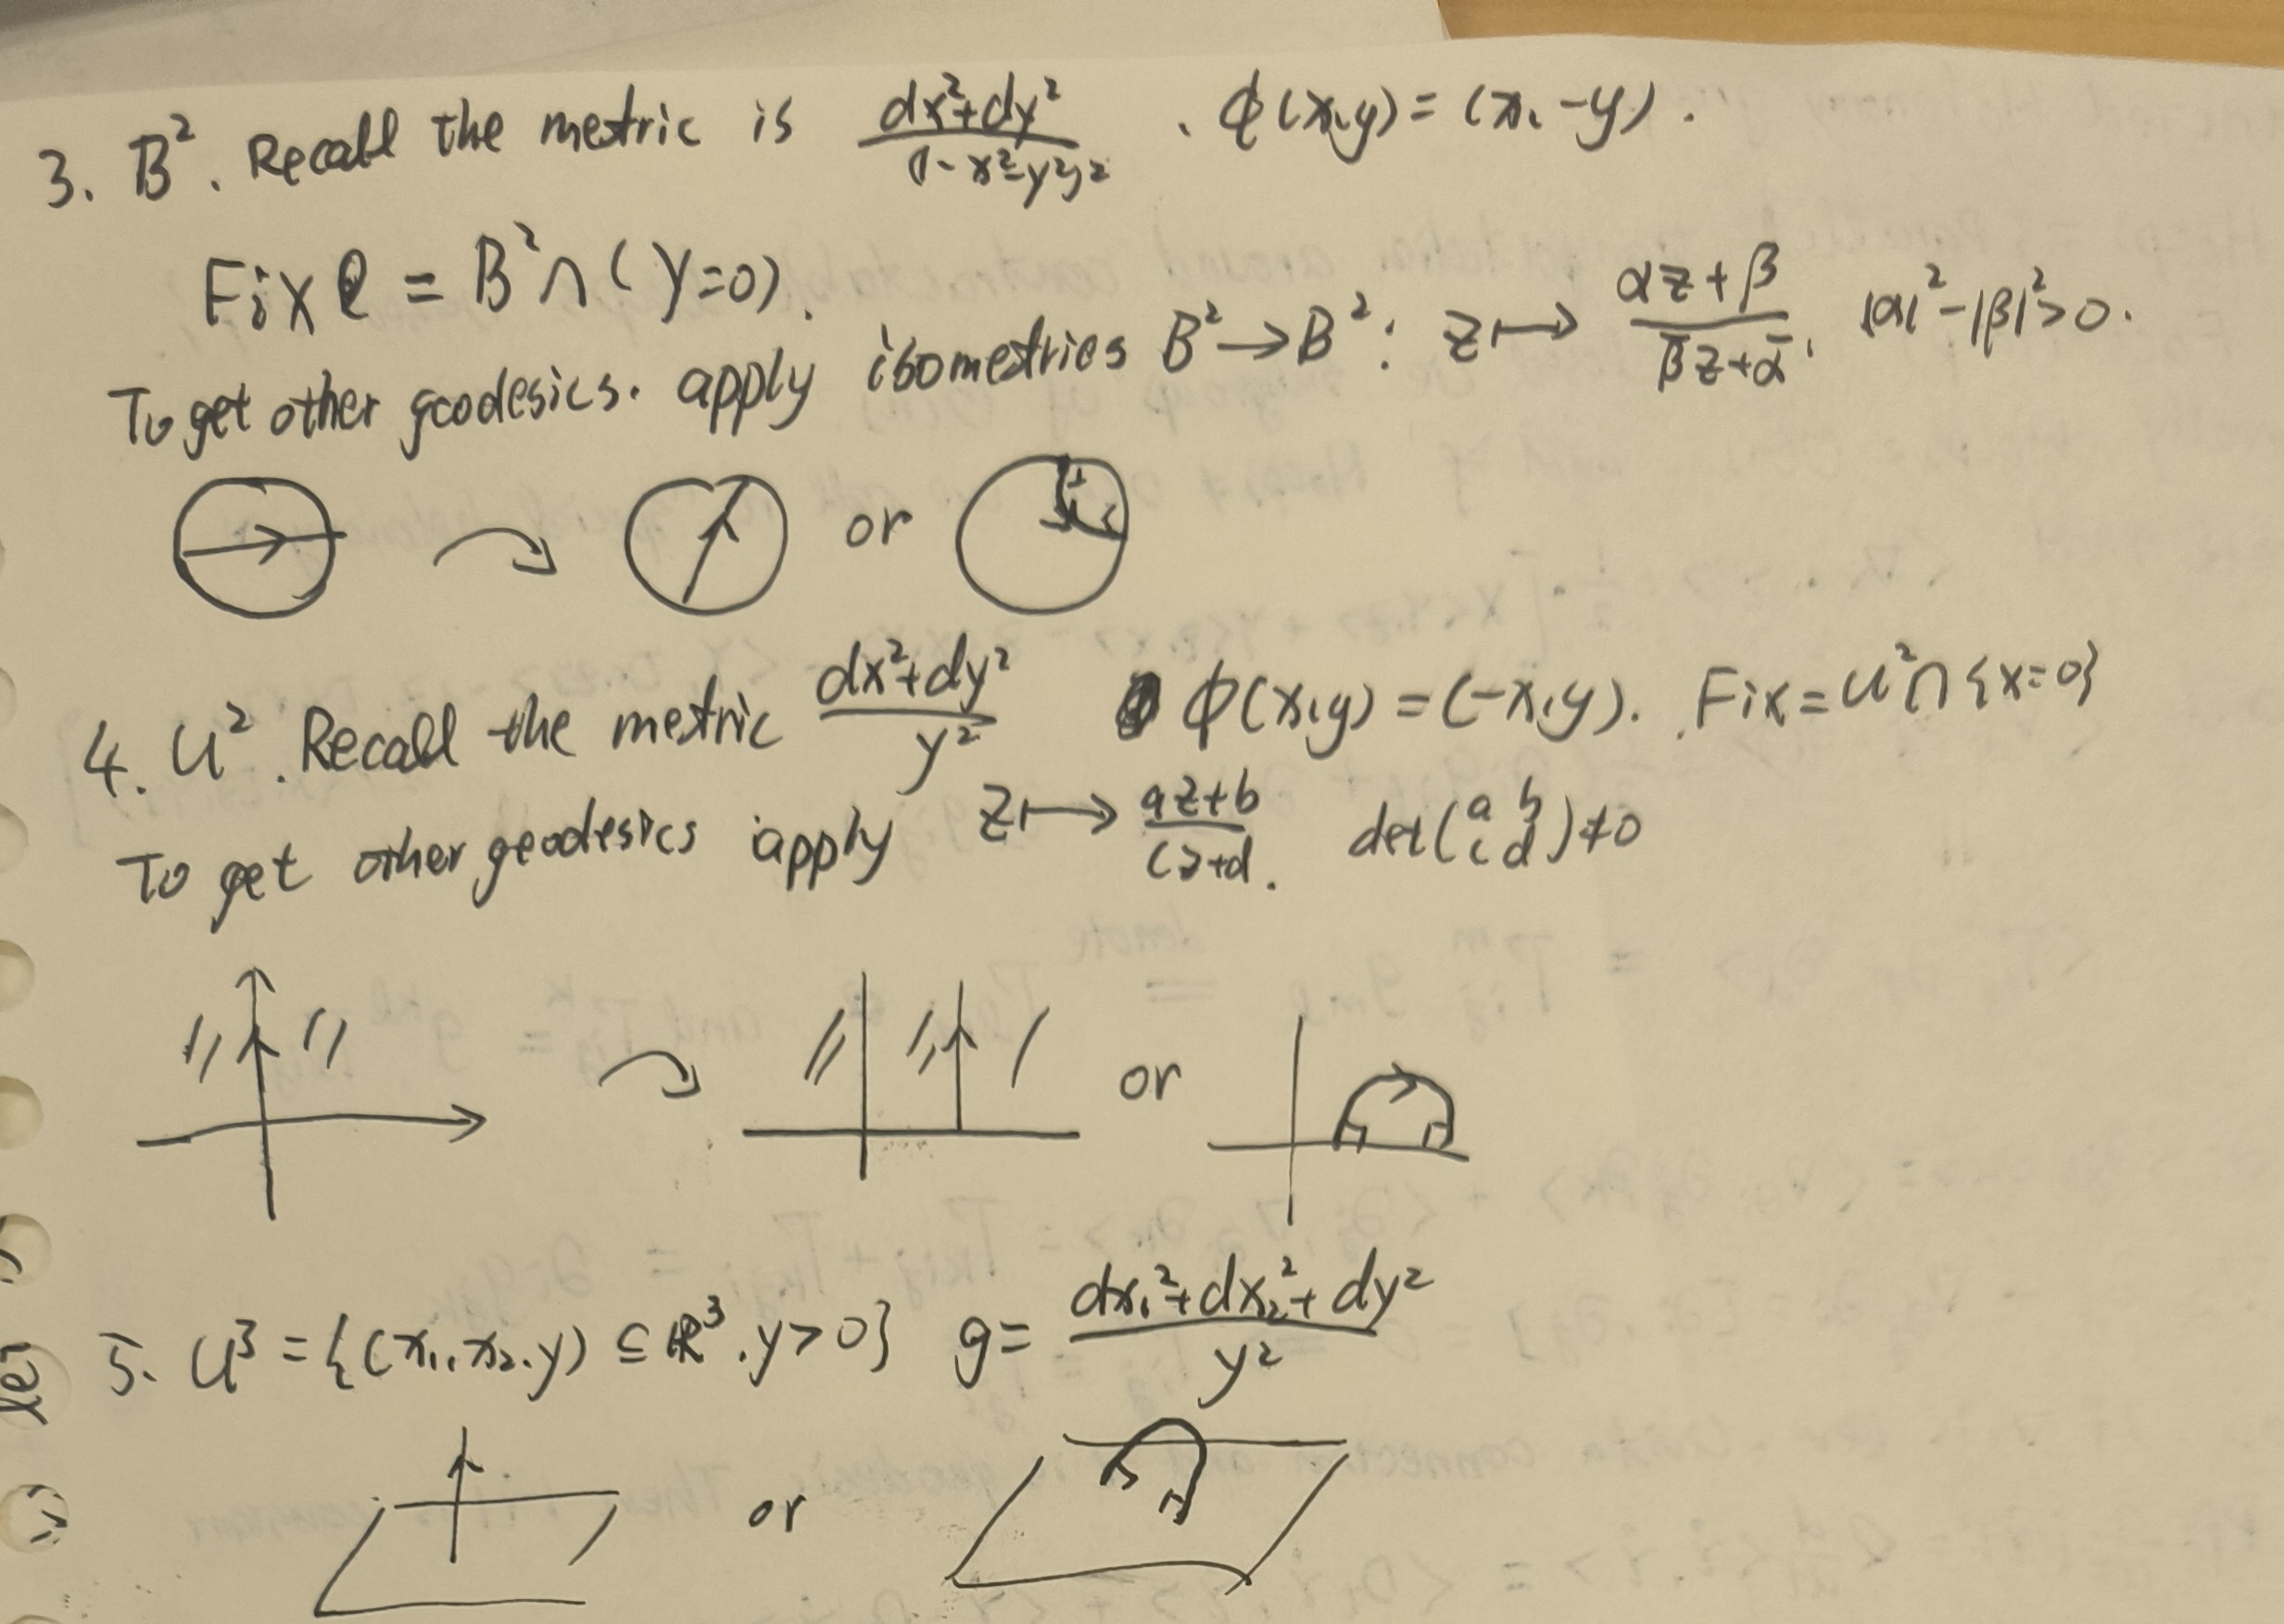
\includegraphics[width=0.8\textwidth]{img1.jpg} % 替换为你的图片文件名（png/jpg/pdf 等）
\end{figure}



\subsection{The Exponential Map}

\textbf{Lemma (Scaling):} For a geodesic $\gamma_v(t)$, we have $\gamma_{cv}(t) = \gamma_v(ct)$.

\textbf{Definition:} Let $\mathcal{E} = \{ v \in TM \mid \gamma_v(1) \text{ is defined} \}$. The \textbf{exponential map} $\exp: \mathcal{E} \to M$ is defined by:
\[ \exp(v) = \gamma_v(1), \quad \exp_p(v) = \exp|_{T_p M}(v) \]

\textbf{Properties of $\exp_p$:}
\begin{enumerate}
    \item $\mathcal{E}$ is an open subset of $TM$ containing the zero section.
    \item $\exp_p(tv) = \gamma_v(t)$.
    \item $\exp_p$ is smooth.
    \item $d(\exp_p)_0: T_0(T_p M) \cong T_p M \to T_p M$ is the identity map.
\end{enumerate}

\textbf{Motivation (Geodesic Flow):}
The geodesic equation $\ddot{x}^k + \Gamma_{ij}^k \dot{x}^i \dot{x}^j = 0$ can be written as a first-order system on $TM$:
\[ \begin{cases} \frac{dx^i}{dt} = v^i \\ \frac{dv^k}{dt} = -\Gamma_{ij}^k v^i v^j \end{cases} \]
This defines a vector field $G$ on $TM$ whose flow gives the geodesics.

\begin{proof}
    \subsubsection*{$\mathcal{E}$ is an Open Subset of $TM$ and $\exp$ is Smooth}

\textbf{Logic from Blackboard 2:}
Let $\Theta_t: \mathcal{D} \to TM$ be the flow generated by the vector field $G$. According to the theory of Ordinary Differential Equations (ODEs), the flow $\Theta_t(v)$ is defined on an open domain $\mathcal{D} \subset \mathbb{R} \times TM$.

We define the domain of the exponential map as:
\[ \mathcal{E} = \{ v \in TM \mid \Theta_t(v) \text{ is defined for } t \in [0, 1] \} \]
If the flow starting from $v$ exists up to time $1$, then by the \textbf{fundamental theorem of ODEs} (continuous dependence on initial conditions), the flow exists up to time $1$ (and "a bit farther") for all vectors in a sufficiently small neighborhood of $v$ in $TM$. Hence, $\mathcal{E}$ is an \textbf{open subset} of $TM$.

Furthermore, since the geodesic vector field $G$ is smooth, its flow $\Theta_t$ is also smooth. The exponential map is defined as the composition:
\[ \exp = \pi \circ \Theta_1 \]
where $\pi: TM \to M$ is the natural projection $(x, v) \mapsto x$. As a composition of smooth maps, $\exp: \mathcal{E} \to M$ is \textbf{smooth}.

\subsubsection*{$\exp_p(tv) = \gamma_v(t)$}

By the definition of the exponential map, $\exp_p(v) = \gamma_v(1)$. 
Recall the \textbf{scaling property} (homogeneity) of geodesics: for any constant $c > 0$, the curve $t \mapsto \gamma_v(ct)$ is a geodesic with initial velocity $c \dot{\gamma}_v(0) = cv$. By uniqueness of geodesics, we have:
\[ \gamma_{cv}(t) = \gamma_v(ct) \]
Setting $c=t$ and evaluating at $1$, we obtain:
\[ \exp_p(tv) = \gamma_{tv}(1) = \gamma_v(t \cdot 1) = \gamma_v(t) \]
This shows that $\exp_p$ maps the line segment in $T_p M$ through the origin to the corresponding geodesic on $M$.

\subsubsection*{The Differential $(d\exp_p)_0 = \text{id}_{T_p M}$}

We wish to compute the derivative of $\exp_p: T_p M \to M$ at the origin $0 \in T_p M$. We identify $T_0(T_p M)$ with $T_p M$ itself. For any $v \in T_p M$, consider the path $c(t) = tv$ in $T_p M$. Note that $c(0)=0$ and $c'(0)=v$.

By the definition of the differential:
\[ (d\exp_p)_0 (v) = \left. \frac{d}{dt} \right|_{t=0} \exp_p(c(t)) = \left. \frac{d}{dt} \right|_{t=0} \exp_p(tv) \]
Using the property derived in the previous section ($\exp_p(tv) = \gamma_v(t)$):
\[ (d\exp_p)_0 (v) = \left. \frac{d}{dt} \right|_{t=0} \gamma_v(t) = \dot{\gamma}_v(0) \]
By the initial conditions of the geodesic $\gamma_v$, we have $\dot{\gamma}_v(0) = v$. 
Therefore:
\[ (d\exp_p)_0 (v) = v \]
which means $(d\exp_p)_0$ is the \textbf{identity map} on $T_p M$.
\end{proof}

\newpage

\section{Lecture 10}



\subsection{Exponential Map and Normal Coordinates}

\textbf{Lemma:} For every $p \in M$, there exists a neighborhood $V$ of $0 \in T_pM$ and a neighborhood $\mathcal{U}$ of $p$ such that $\exp_p: V \to \mathcal{U}$ is a diffeomorphism.

\textbf{Definition (Normal Neighborhood):} A neighborhood of $p$ is called a \textbf{normal neighborhood} if it is the diffeomorphic image of a star-shaped neighborhood of $0 \in T_pM$ under $\exp_p$.

\textbf{Definition (Geodesic Ball):} If $\varepsilon > 0$ is small enough such that $\exp_p: B_\varepsilon(0) \to B_\varepsilon(p)$ is a diffeomorphism, $B_\varepsilon(p)$ is called a \textbf{geodesic ball}. Its boundary is the \textbf{geodesic sphere}.

\subsection*{Riemannian Normal Coordinates (RNC)}
Let $\{E_i\}$ be an orthonormal basis for $T_pM$. The coordinate map is $(x^i) \mapsto \exp_p(\sum x^i E_i)$.
\textbf{Properties:}
\begin{enumerate}
    \item $p$ has coordinates $(0, \dots, 0)$.
    \item Geodesics through $p$ are radial lines: $x^i(t) = tv^i$.
    \item At the origin: $g_{ij}(0) = \delta_{ij}$.
    \item At the origin: $\Gamma_{ij}^k(0) = 0$.
\end{enumerate}

\begin{proof}
1.2 are automatic.

3. Consider the pull back metric $\exp_p^* g$, we aim to show that $\exp_p^* g(0) = \delta_{ij}$. For $V = V^i\frac{\p}{\p x^i}\in T_0 T_p M$.
Put $\gamma(t) = tV$, $\exp_p(\gamma(t)) = \gamma_V(t)$. Then $(d\exp_p)_0(V) = \dot{\gamma}_V(0) = V$, i.e. 
\[\exp_p^*g_0(V,V) = \|V\|^2 \Longrightarrow \exp_p^*g_0 = \delta_{ij}.\]



4. Let $\gamma(t) = tv$ be a geodesic. The geodesic equation is $\ddot{x}^i + \Gamma_{jk}^i \dot{x}^j \dot{x}^k = 0$.
Substituting $x^i(t) = tv^i$, we have $0 + \Gamma_{jk}^i(0) v^j v^k = 0$. Since this holds for all $v \in T_pM$ and $\Gamma_{jk}^i$ is symmetric, $\Gamma_{jk}^i(0) = 0$.
\end{proof}

\subsection{Uniformly Normal Neighborhoods}

\textbf{Definition:} An open set $W \subset M$ is \textbf{uniformly normal} if there exists $\delta > 0$ such that for any $w \in W$, $W \subset \exp_w(B_\delta(0))$, and $\exp_w$ is a diffeomorphism on $B_\delta(0)$.

\textbf{Proposition:} Every $p \in M$ has a uniformly normal neighborhood.

\begin{proof}
Define the map $F: \mathcal{E} \to M \times M$ by $F(q, v) = (q, \exp_q v)$, where $\mathcal{E} \subset TM$ is the open domain where the exponential map is defined. We want to show that $dF_{(p,0)}$ is an isomorphism.

Recall that the tangent space $T_{(p,0)}TM$ fits into a short exact sequence involving the vertical space (tangent to the fiber $T_p M$) and the horizontal space (projecting to $T_p M$ via $d\pi$). The tangent space to the product manifold is $T_{(p,p)}(M \times M) \cong T_p M \oplus T_p M$. 

We can construct the following diagram:
\[
\begin{tikzcd}
    0 \arrow[r] & T_p M \arrow[r, "i_*"] \arrow[d, "\text{id}"] & T_{(p,0)} TM \arrow[r, "d\pi"] \arrow[d, "dF_{(p,0)}"] & T_p M \arrow[r] \arrow[d, "\text{id}"] & 0 \\
    0 \arrow[r] & T_p M \arrow[r, "0 \oplus \text{id}"] & T_{(p,p)}(M \times M) \arrow[r, "d\text{pr}_1"] & T_p M \arrow[r] & 0
\end{tikzcd}
\]
Let us verify that this diagram commutes:
\begin{itemize}
    \item \textbf{Left Square:} For any $v \in T_p M$, the vertical lift $i_*(v)$ is the tangent vector to the curve $c(t) = (p, tv)$ in $TM$ at $t=0$. Applying the differential $dF$, we have:
    \[
    dF_{(p,0)}(i_*(v)) = \left. \frac{d}{dt} \right|_{t=0} F(p, tv) = \left. \frac{d}{dt} \right|_{t=0} (p, \exp_p(tv)) = (0, v)
    \]
    which exactly matches the map $0 \oplus \text{id}$ in the bottom row. Hence, the left square commutes.
    \item \textbf{Right Square:} Notice that for any $(q,v) \in TM$, projecting the first component gives $\text{pr}_1(F(q,v)) = \text{pr}_1(q, \exp_q v) = q = \pi(q,v)$. Taking the differential of both sides at $(p,0)$ yields $d\text{pr}_1 \circ dF_{(p,0)} = d\pi$, meaning the right square commutes.
\end{itemize}

Since the rows are exact and the two outer vertical maps are isomorphisms (they are identity maps), the \textbf{Five Lemma} implies that the middle map $dF_{(p,0)}: T_{(p,0)}TM \to T_{(p,p)}(M \times M)$ is a linear isomorphism.

By the \textbf{Inverse Function Theorem}, $F$ is a local diffeomorphism at $(p,0)$. Thus, there exists a neighborhood $V \subset TM$ of $(p,0)$ that is mapped diffeomorphically onto a neighborhood of $(p,p)$ in $M \times M$.

We can choose a sufficiently small open neighborhood $W \subset M$ of $p$ and a radius $\delta > 0$ such that $W \times W \subset F(V \cap \{|v| < \delta\})$. 
Then, for any pair $(w, w') \in W \times W$, there exists a unique tangent vector $v \in T_w M$ with $|v| < \delta$ such that $F(w, v) = (w, w')$. By definition of $F$, this means $\exp_w(v) = w'$.

Furthermore, because $F$ is a diffeomorphism on this restricted domain, for each fixed $w \in W$, the map $\exp_w$ acts as a diffeomorphism from the $\delta$-ball $B_\delta(0) \subset T_w M$ onto its image, which completely contains $W$. Therefore, $W$ is uniformly normal.
\end{proof}

\subsection{Geodesic as length-minimizing curves}

\textbf{Recall:} regular curve $\dot{\gamma} \neq 0$, admissible curve: piecewise regular curve.

\vspace{1em}
\noindent
\textbf{Def:} Given intervals $I, J \in \mathbb{R}$. A 1-parameter family of curves is a continuous map $\Gamma : J \times I \to M$. 
We write $\Gamma_s(t) = \Gamma(s, t)$ be a curve for each $s$.

\vspace{1em}
\noindent
\textbf{Def:} A vector field along $\Gamma$ is a continuous map $V : J \times I \to TM$ s.t. $\pi \circ V = \Gamma$.

\vspace{1em}
\noindent
\textbf{Def:} A 1-parameter family of curves is admissible if
\begin{enumerate}
    \item $J$ is open and $I = [a, b]$.
    \item $\exists$ partition $a = a_0 < a_1 < \dots < a_k = b$, so $\Gamma$ is smooth on $J \times [a_{i-1}, a_i]$.
    \item $\Gamma_s(t)$ is admissible for each $s$.
\end{enumerate}

\noindent
\textbf{Note:} $\partial_t \Gamma$ may not be vector field along $\Gamma$, but $\partial_s \Gamma$ is.

\vspace{1em}
\noindent
\textbf{Def:} Given $\gamma: [a, b] \to M$, a variation of $\gamma$ is a 1-parameter family of curves (admissible), and $\Gamma(0, t) = \gamma(t)$.

\vspace{1em}
\noindent
\textbf{Def:} If $\Gamma$ is a variation of $\gamma$, then the variation field of $\gamma$ is the piecewise smooth vector field 
\[ V(t) = \frac{\partial \Gamma}{\partial s}(0, t) \quad \text{along } \gamma. \]

\noindent
\textbf{Def:} A vector field along $\gamma$ is proper if $V(a) = V(b) = 0$.

\vspace{1em}
\noindent
\textbf{Note:} If $\Gamma$ is proper variation of $\gamma$, then the variation field is proper vector along $\gamma$.

\vspace{1em}
\noindent
\textbf{Lemma:} If $\gamma$ is admissible, and $V$ is vector field along $\gamma$, then $\exists$ variation $\Gamma$ of $\gamma$, so $V$ is its variation field. \\
If $V$ is proper then we can make $\Gamma$ be proper.

\vspace{2em}
\hrule
\vspace{2em}

\noindent
\textbf{Lemma:} On rectangles $J \times [a_{i-1}, a_i]$,
\[ D_s \partial_t \Gamma = D_t \partial_s \Gamma. \]

\noindent
\textbf{Pf:} Say $\Gamma$ lives in a coord nbhd. $\Gamma(s, t) = (x^1(s, t), \dots, x^n(s, t))$.
\[ \partial_t \Gamma = \sum \frac{\partial x^i}{\partial t} \partial_i, \quad \partial_s \Gamma = \sum \frac{\partial x^i}{\partial s} \partial_i \]
\[ D_t V = \sum \left( \frac{dv^i}{dt} + \Gamma_{jk}^i \frac{dx^j}{dt} v^k \right) \partial_i \]
Hence,
\[ D_s \partial_t \Gamma = \sum \left( \frac{\partial^2 x^i}{\partial s \partial t} + \Gamma_{jk}^i \frac{\partial x^j}{\partial s} \frac{\partial x^k}{\partial t} \right) \partial_i \]
which is symmetric in $s, t$.
\end{comment}

\section{Lecture 9}

\subsection{Holonomy Groups}

\begin{definition}[Restricted Holonomy Group]
The restricted holonomy group $\text{Hol}_0(p)$ consists of parallel translations around contractible loops based at $p$.
\end{definition}


\noindent\textbf{fact:}$\text{Hol}_0(p)$ is the identity component of $\text{Hol}(p)$. It is a connected, closed Lie subgroup of $SO(n)$.


\begin{definition}[Special Holonomy]
Generally, $\text{Hol}(p) = O(n)$. If $\text{Hol}(p) \subsetneq O(n)$, the manifold is said to have \textit{special holonomy} (e.g., K\"ahler, G2, etc.).
\end{definition}

\subsection{Levi-Civita Connection and Christoffel Symbols}

\begin{theorem}[Koszul Formula]
The unique Levi-Civita connection is determined by:
\[ 2\langle \nabla_X Y, Z \rangle = X\langle Y, Z \rangle + Y\langle Z, X \rangle - Z\langle X, Y \rangle + \langle [X, Y], Z \rangle - \langle [Y, Z], X \rangle + \langle [Z, X], Y \rangle \]
\end{theorem}

\begin{remark}[In Local Coordinates]
Let $\partial_i$ be coordinate vectors. Then $\langle \nabla_{\partial_i} \partial_j, \partial_l \rangle = \frac{1}{2}(\partial_i g_{jl} + \partial_j g_{il} - \partial_l g_{ij})$.
We define the Christoffel symbols of the first and second kind:
\[ \Gamma_{ijl} = \langle \nabla_{\partial_i} \partial_j, \partial_l \rangle, \quad \nabla_{\partial_i} \partial_j = \Gamma_{ij}^k \partial_k \implies \Gamma_{ij}^k = g^{kl} \Gamma_{ijl} \]
\end{remark}

\begin{remark}[Symmetry]
Since $\nabla_{\partial_i} \partial_j - \nabla_{\partial_j} \partial_i = [\partial_i, \partial_j] = 0$, we have $\Gamma_{ij}^k = \Gamma_{ji}^k$.
\end{remark}

\subsection{Properties of Geodesics}

\begin{proposition}
If $\nabla$ is the Levi-Civita connection and $\gamma$ is a geodesic, then $|\dot{\gamma}|$ is constant.
\end{proposition}

\begin{proof}
$\frac{d}{dt} |\dot{\gamma}|^2 = \frac{d}{dt} \langle \dot{\gamma}, \dot{\gamma} \rangle = 2 \langle D_t \dot{\gamma}, \dot{\gamma} \rangle$. Since $\gamma$ is a geodesic, $D_t \dot{\gamma} = 0$, hence the derivative is zero.
\end{proof}

\subsection{Isometries and Geodesics}

\begin{proposition}
If $\phi: M \to \tilde{M}$ is an isometry, then:
\begin{enumerate}
    \item $\phi_* (\nabla_X Y) = \tilde{\nabla}_{\phi_* X} \phi_* Y$. (Isometries preserve the Levi-Civita connection).
    \item $\gamma$ is a geodesic on $M \iff \phi \circ \gamma$ is a geodesic on $\tilde{M}$.
\end{enumerate}
\end{proposition}
\newcommand{\tnba}{\tilde{\nabla}}

\begin{proof}
    \textbf{(1)} First, define $\phi_*\tnba$ by $(\phi_*\tnba)_X Y = \phi_*^{-1}(\tnba_{\phi_* X} \phi_* Y)$, and proof that it is a 
    metric-compatible, torsion-free connection. Hence by unuqueness of Levi-Civita connection, $\phi_*\tnba = \nabla$.

    \textbf{(2)} Trivial.
\end{proof}


\begin{proposition}[Symmetry and Geodesics]
If $\phi \in \text{Isom}(M)$ satisfies $\phi(p)=p$ and $d\phi_p(X)=X$, then the maximal geodesic $\gamma$ with $\gamma(0)=p, \dot{\gamma}(0)=X$ is pointwise fixed by $\phi$, i.e., $\phi(\gamma(t)) = \gamma(t)$.
\end{proposition}

\begin{example}[$S^n$]
Reflection through a 2-plane $P$ spanned by $p, X$. The fixed point set $P \cap S^n$ is a great circle (geodesic).
\end{example}

\begin{example}[$\mathbb{H}^n, \mathbb{B}^2, \mathbb{U}^2$]
Geodesics are obtained as fixed point sets of reflections (lines or circles orthogonal to the boundary).
\end{example}

\begin{figure}[htbp]
  \centering
  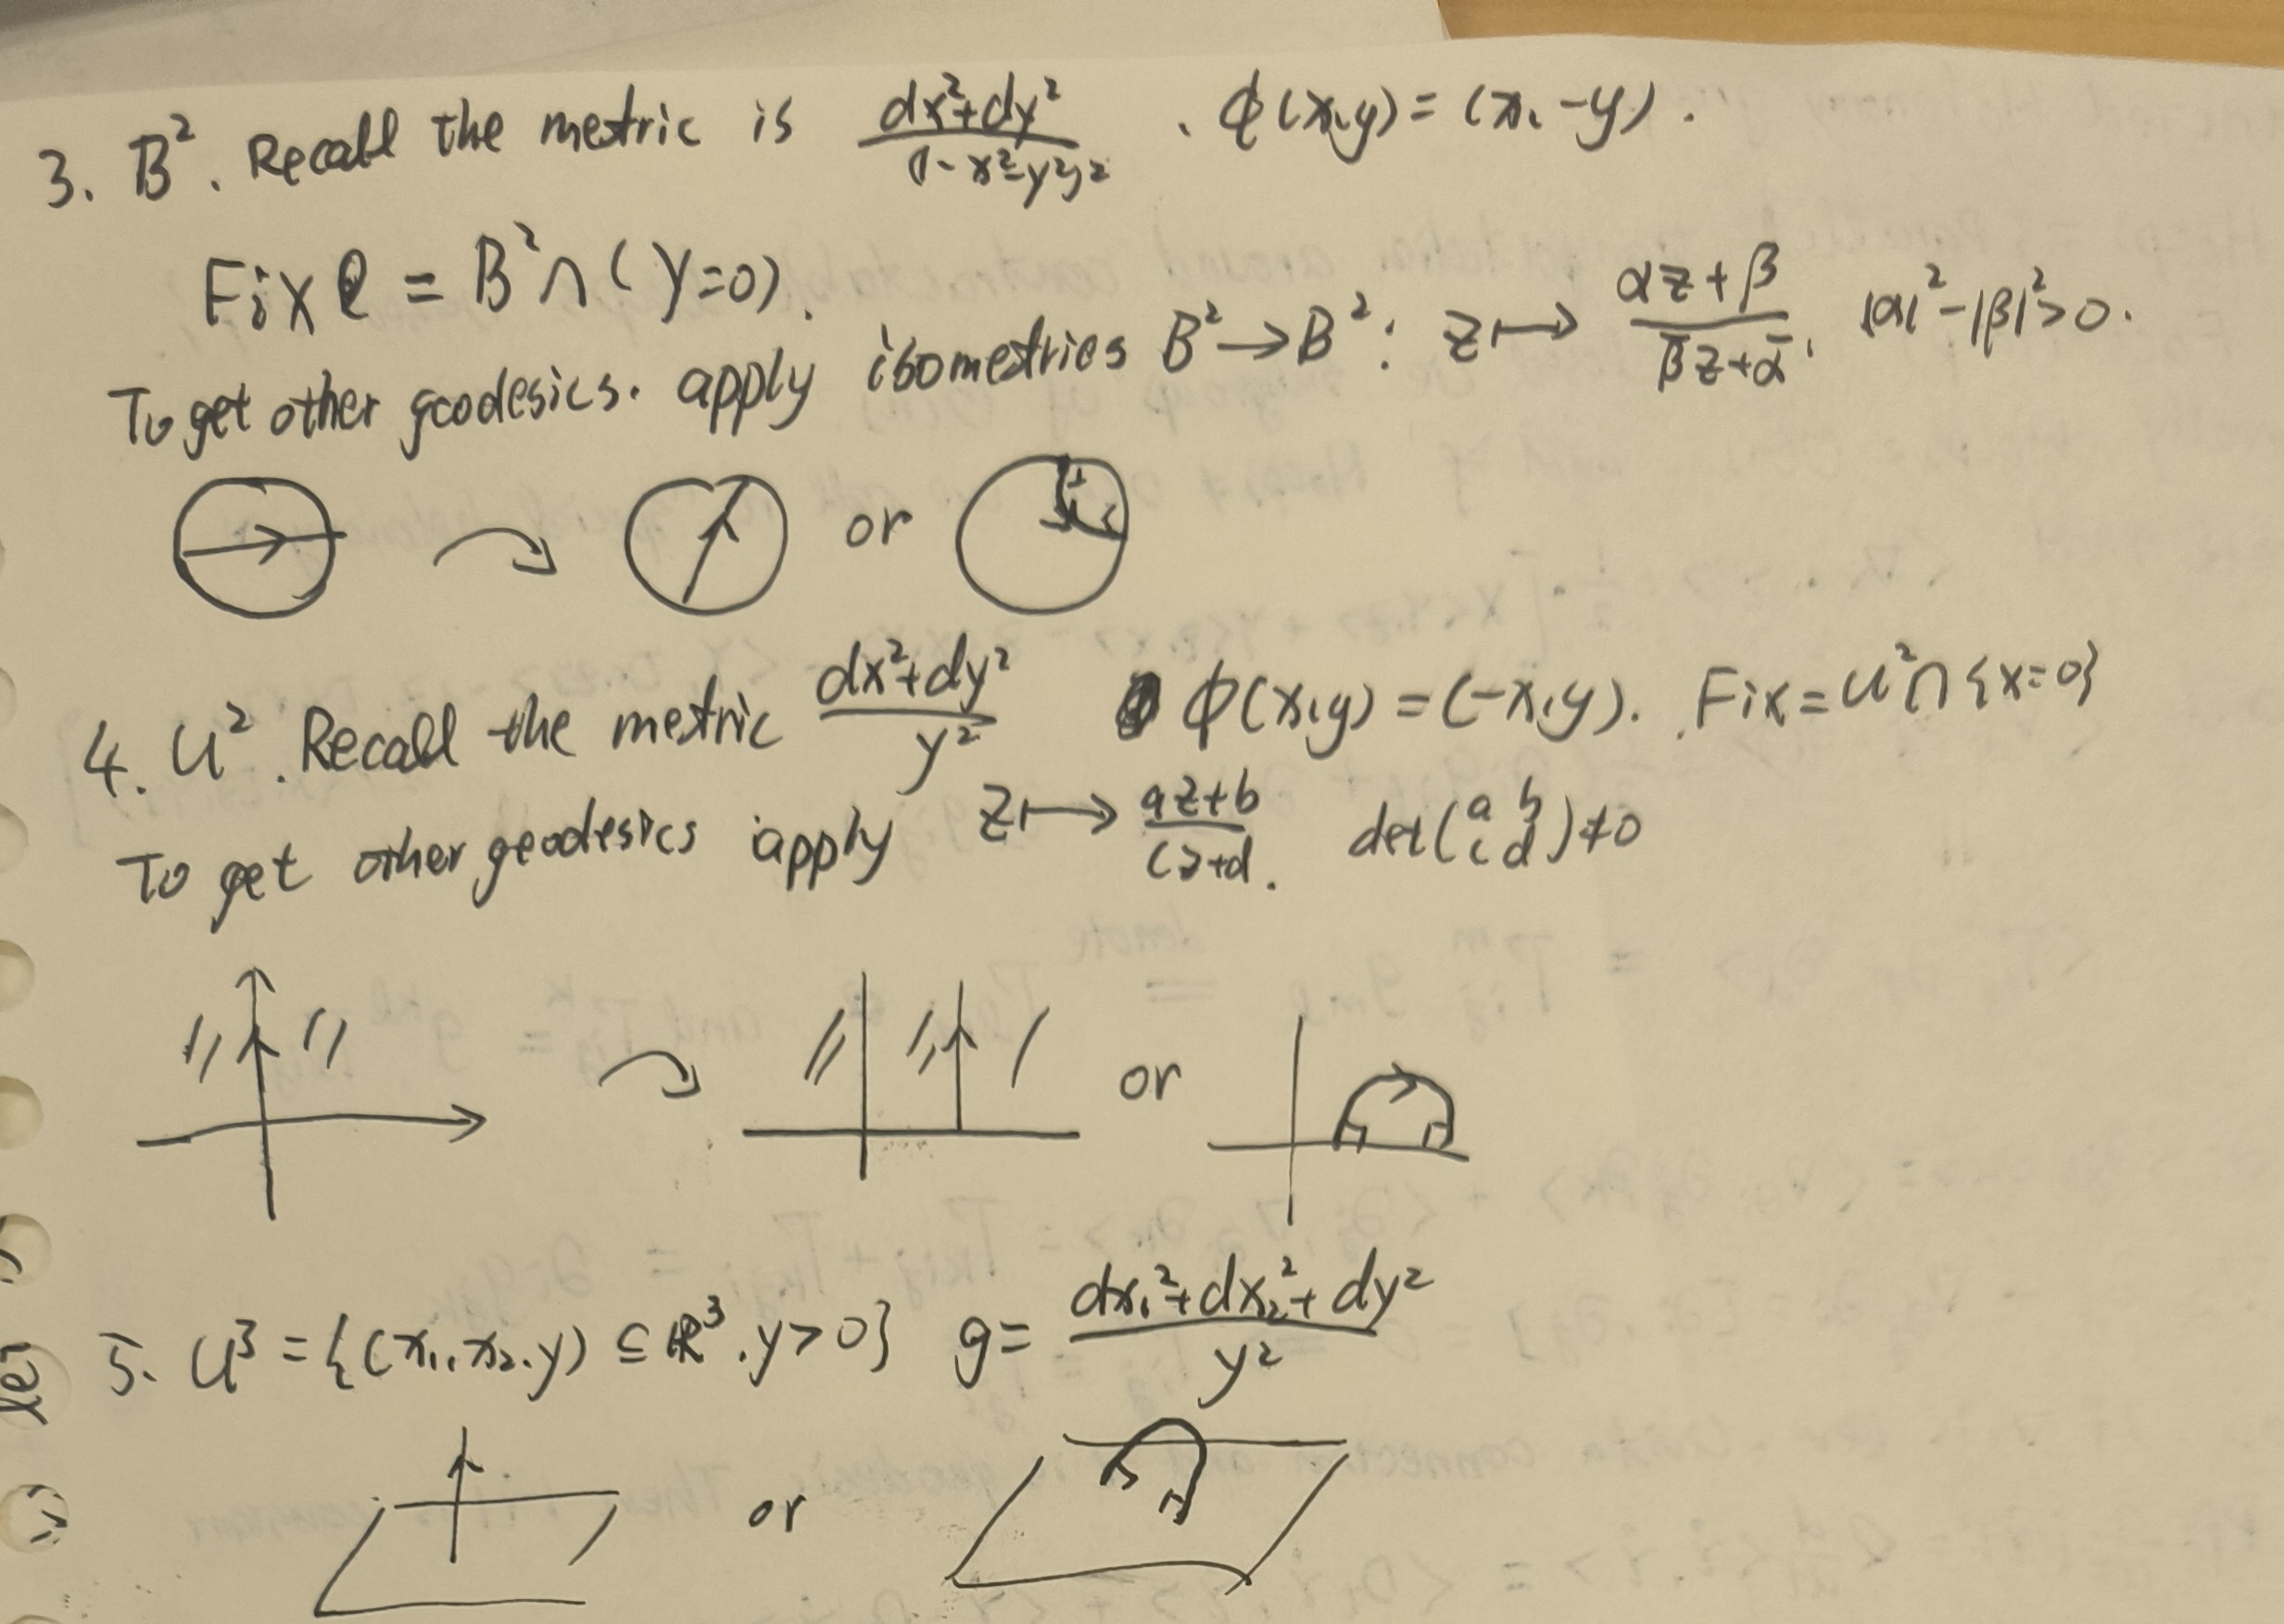
\includegraphics[width=0.8\textwidth]{img1.jpg} % 替换为你的图片文件名（png/jpg/pdf 等）
\end{figure}

\subsection{The Exponential Map}

\begin{lemma}[Scaling]
For a geodesic $\gamma_v(t)$, we have $\gamma_{cv}(t) = \gamma_v(ct)$.
\end{lemma}

\begin{definition}[Exponential Map]
Let $\mathcal{E} = \{ v \in TM \mid \gamma_v(t) \text{ is defined for } t \in [0, 1] \}$. The \textbf{exponential map} $\exp: \mathcal{E} \to M$ is defined by:
\[ \exp(v) = \gamma_v(1), \quad \exp_p(v) = \exp|_{T_p M}(v) \]
\end{definition}

\begin{proposition}[Properties of $\exp_p$]
\begin{enumerate}
    \item $\mathcal{E}$ is an open subset of $TM$ containing the zero section.
    \item $\exp_p(tv) = \gamma_v(t)$.
    \item $\exp_p$ is smooth.
    \item $d(\exp_p)_0: T_0(T_p M) \cong T_p M \to T_p M$ is the identity map.
\end{enumerate}
\end{proposition}

\begin{remark}[Motivation: Geodesic Flow]
The geodesic equation $\ddot{x}^k + \Gamma_{ij}^k \dot{x}^i \dot{x}^j = 0$ can be written as a first-order system on $TM$:
\[ \begin{cases} \frac{dx^i}{dt} = v^i \\ \frac{dv^k}{dt} = -\Gamma_{ij}^k v^i v^j \end{cases} \]
This defines a vector field $G$ on $TM$ whose flow gives the geodesics.
\end{remark}

\begin{proof}[Proof of Properties of $\exp_p$]
\vspace{0.5em}\noindent\textbf{$\mathcal{E}$ is an Open Subset of $TM$ and $\exp$ is Smooth:} \\
\textbf{Logic from Blackboard 2:}
Let $\Theta_t: \mathcal{D} \to TM$ be the flow generated by the vector field $G$. According to the theory of Ordinary Differential Equations (ODEs), the flow $\Theta_t(v)$ is defined on an open domain $\mathcal{D} \subset \mathbb{R} \times TM$.

We define the domain of the exponential map as:
\[ \mathcal{E} = \{ v \in TM \mid \Theta_t(v) \text{ is defined for } t \in [0, 1] \} \]
If the flow starting from $v$ exists up to time $1$, then by the \textbf{fundamental theorem of ODEs} (continuous dependence on initial conditions), the flow exists up to time $1$ (and "a bit farther") for all vectors in a sufficiently small neighborhood of $v$ in $TM$. Hence, $\mathcal{E}$ is an \textbf{open subset} of $TM$.

Furthermore, since the geodesic vector field $G$ is smooth, its flow $\Theta_t$ is also smooth. The exponential map is defined as the composition:
\[ \exp = \pi \circ \Theta_1 \]
where $\pi: TM \to M$ is the natural projection $(x, v) \mapsto x$. As a composition of smooth maps, $\exp: \mathcal{E} \to M$ is \textbf{smooth}.

\vspace{0.5em}\noindent\textbf{$\exp_p(tv) = \gamma_v(t)$:} \\
By the definition of the exponential map, $\exp_p(v) = \gamma_v(1)$. 
Recall the \textbf{scaling property} (homogeneity) of geodesics: for any constant $c > 0$, the curve $t \mapsto \gamma_v(ct)$ is a geodesic with initial velocity $c \dot{\gamma}_v(0) = cv$. By uniqueness of geodesics, we have:
\[ \gamma_{cv}(t) = \gamma_v(ct) \]
Setting $c=t$ and evaluating at $1$, we obtain:
\[ \exp_p(tv) = \gamma_{tv}(1) = \gamma_v(t \cdot 1) = \gamma_v(t) \]
This shows that $\exp_p$ maps the line segment in $T_p M$ through the origin to the corresponding geodesic on $M$.

\vspace{0.5em}\noindent\textbf{The Differential $(d\exp_p)_0 = \text{id}_{T_p M}$:} \\
We wish to compute the derivative of $\exp_p: T_p M \to M$ at the origin $0 \in T_p M$. We identify $T_0(T_p M)$ with $T_p M$ itself. For any $v \in T_p M$, consider the path $c(t) = tv$ in $T_p M$. Note that $c(0)=0$ and $c'(0)=v$.

By the definition of the differential:
\[ (d\exp_p)_0 (v) = \left. \frac{d}{dt} \right|_{t=0} \exp_p(c(t)) = \left. \frac{d}{dt} \right|_{t=0} \exp_p(tv) \]
Using the property derived in the previous section ($\exp_p(tv) = \gamma_v(t)$):
\[ (d\exp_p)_0 (v) = \left. \frac{d}{dt} \right|_{t=0} \gamma_v(t) = \dot{\gamma}_v(0) \]
By the initial conditions of the geodesic $\gamma_v$, we have $\dot{\gamma}_v(0) = v$. 
Therefore:
\[ (d\exp_p)_0 (v) = v \]
which means $(d\exp_p)_0$ is the \textbf{identity map} on $T_p M$.
\end{proof}

\newpage

\section{Lecture 10}

\subsection{Exponential Map and Normal Coordinates}

\begin{lemma}
For every $p \in M$, there exists a neighborhood $V$ of $0 \in T_pM$ and a neighborhood $\mathcal{U}$ of $p$ such that $\exp_p: V \to \mathcal{U}$ is a diffeomorphism.
\end{lemma}

\begin{definition}[Normal Neighborhood]
A neighborhood of $p$ is called a \textbf{normal neighborhood} if it is the diffeomorphic image of a star-shaped neighborhood of $0 \in T_pM$ under $\exp_p$.
\end{definition}

\begin{definition}[Geodesic Ball]
If $\varepsilon > 0$ is small enough such that $\exp_p: B_\varepsilon(0) \to B_\varepsilon(p)$ is a diffeomorphism, $B_\varepsilon(p)$ is called a \textbf{geodesic ball}. Its boundary is the \textbf{geodesic sphere}.
\end{definition}

\subsection*{Riemannian Normal Coordinates (RNC)}
Let $\{E_i\}$ be an orthonormal basis for $T_pM$. The coordinate map is $(x^i) \mapsto \exp_p(\sum x^i E_i)$.

\begin{proposition}[Properties of RNC]
\begin{enumerate}
    \item $p$ has coordinates $(0, \dots, 0)$.
    \item Geodesics through $p$ are radial lines: $x^i(t) = tv^i$.
    \item At the origin: $g_{ij}(0) = \delta_{ij}$.
    \item At the origin: $\Gamma_{ij}^k(0) = 0$.
\end{enumerate}
\end{proposition}

\begin{proof}
1 and 2 are automatic.

3. Consider the pull back metric $\exp_p^* g$, we aim to show that $\exp_p^* g(0) = \delta_{ij}$. For $V = V^i\frac{\partial}{\partial x^i}\in T_0 T_p M$.
Put $\gamma(t) = tV$, $\exp_p(\gamma(t)) = \gamma_V(t)$. Then $(d\exp_p)_0(V) = \dot{\gamma}_V(0) = V$, i.e. 
\[\exp_p^*g_0(V,V) = \|V\|^2 \Longrightarrow \exp_p^*g_0 = \delta_{ij}.\]

4. Let $\gamma(t) = tv$ be a geodesic. The geodesic equation is $\ddot{x}^i + \Gamma_{jk}^i \dot{x}^j \dot{x}^k = 0$.
Substituting $x^i(t) = tv^i$, we have $0 + \Gamma_{jk}^i(0) v^j v^k = 0$. Since this holds for all $v \in T_pM$ and $\Gamma_{jk}^i$ is symmetric, $\Gamma_{jk}^i(0) = 0$.
\end{proof}

\subsection{Uniformly Normal Neighborhoods}

\begin{definition}[Uniformly Normal Neighborhood]
An open set $W \subset M$ is \textbf{uniformly normal} if there exists $\delta > 0$ such that for any $w \in W$, $W \subset \exp_w(B_\delta(0))$, and $\exp_w$ is a diffeomorphism on $B_\delta(0)$.
\end{definition}

\begin{proposition}
Every $p \in M$ has a uniformly normal neighborhood.
\end{proposition}

\begin{proof}
Define the map $F: \mathcal{E} \to M \times M$ by $F(q, v) = (q, \exp_q v)$, where $\mathcal{E} \subset TM$ is the open domain where the exponential map is defined. We want to show that $dF_{(p,0)}$ is an isomorphism.

Recall that the tangent space $T_{(p,0)}TM$ fits into a short exact sequence involving the vertical space (tangent to the fiber $T_p M$) and the horizontal space (projecting to $T_p M$ via $d\pi$). The tangent space to the product manifold is $T_{(p,p)}(M \times M) \cong T_p M \oplus T_p M$. 

We can construct the following diagram:
\[
\begin{tikzcd}
    0 \arrow[r] & T_p M \arrow[r, "i_*"] \arrow[d, "\text{id}"] & T_{(p,0)} TM \arrow[r, "d\pi"] \arrow[d, "dF_{(p,0)}"] & T_p M \arrow[r] \arrow[d, "\text{id}"] & 0 \\
    0 \arrow[r] & T_p M \arrow[r, "0 \oplus \text{id}"] & T_{(p,p)}(M \times M) \arrow[r, "d\text{pr}_1"] & T_p M \arrow[r] & 0
\end{tikzcd}
\]
Let us verify that this diagram commutes:
\begin{itemize}
    \item \textbf{Left Square:} For any $v \in T_p M$, the vertical lift $i_*(v)$ is the tangent vector to the curve $c(t) = (p, tv)$ in $TM$ at $t=0$. Applying the differential $dF$, we have:
    \[
    dF_{(p,0)}(i_*(v)) = \left. \frac{d}{dt} \right|_{t=0} F(p, tv) = \left. \frac{d}{dt} \right|_{t=0} (p, \exp_p(tv)) = (0, v)
    \]
    which exactly matches the map $0 \oplus \text{id}$ in the bottom row. Hence, the left square commutes.
    \item \textbf{Right Square:} Notice that for any $(q,v) \in TM$, projecting the first component gives $\text{pr}_1(F(q,v)) = \text{pr}_1(q, \exp_q v) = q = \pi(q,v)$. Taking the differential of both sides at $(p,0)$ yields $d\text{pr}_1 \circ dF_{(p,0)} = d\pi$, meaning the right square commutes.
\end{itemize}

Since the rows are exact and the two outer vertical maps are isomorphisms (they are identity maps), the \textbf{Five Lemma} implies that the middle map $dF_{(p,0)}: T_{(p,0)}TM \to T_{(p,p)}(M \times M)$ is a linear isomorphism.

By the \textbf{Inverse Function Theorem}, $F$ is a local diffeomorphism at $(p,0)$. Thus, there exists a neighborhood $V \subset TM$ of $(p,0)$ that is mapped diffeomorphically onto a neighborhood of $(p,p)$ in $M \times M$.

We can choose a sufficiently small open neighborhood $W \subset M$ of $p$ and a radius $\delta > 0$ such that $W \times W \subset F(V \cap \{|v| < \delta\})$. 
Then, for any pair $(w, w') \in W \times W$, there exists a unique tangent vector $v \in T_w M$ with $|v| < \delta$ such that $F(w, v) = (w, w')$. By definition of $F$, this means $\exp_w(v) = w'$.

Furthermore, because $F$ is a diffeomorphism on this restricted domain, for each fixed $w \in W$, the map $\exp_w$ acts as a diffeomorphism from the $\delta$-ball $B_\delta(0) \subset T_w M$ onto its image, which completely contains $W$. Therefore, $W$ is uniformly normal.
\end{proof}

\subsection{Geodesic as length-minimizing curves}

\begin{remark}[Recall]
Regular curve $\dot{\gamma} \neq 0$, admissible curve: piecewise regular curve.
\end{remark}

\begin{definition}
Given intervals $I, J \in \mathbb{R}$. A 1-parameter family of curves is a continuous map $\Gamma : J \times I \to M$. 
We write $\Gamma_s(t) = \Gamma(s, t)$ be a curve for each $s$.
\end{definition}

\begin{definition}
A vector field along $\Gamma$ is a continuous map $V : J \times I \to TM$ s.t. $\pi \circ V = \Gamma$.
\end{definition}

\begin{definition}
A 1-parameter family of curves is admissible if:
\begin{enumerate}
    \item $J$ is open and $I = [a, b]$.
    \item $\exists$ partition $a = a_0 < a_1 < \dots < a_k = b$, so $\Gamma$ is smooth on $J \times [a_{i-1}, a_i]$.
    \item $\Gamma_s(t)$ is admissible for each $s$.
\end{enumerate}
\end{definition}

\begin{remark}
$\partial_t \Gamma$ may not be a vector field along $\Gamma$, but $\partial_s \Gamma$ is.
\end{remark}

\begin{definition}
Given $\gamma: [a, b] \to M$, a variation of $\gamma$ is a 1-parameter family of curves (admissible), and $\Gamma(0, t) = \gamma(t)$.
\end{definition}

\begin{definition}
If $\Gamma$ is a variation of $\gamma$, then the variation field of $\gamma$ is the piecewise smooth vector field 
\[ V(t) = \frac{\partial \Gamma}{\partial s}(0, t) \quad \text{along } \gamma. \]
\end{definition}

\begin{definition}
A vector field along $\gamma$ is proper if $V(a) = V(b) = 0$.
\end{definition}

\begin{remark}
If $\Gamma$ is a proper variation of $\gamma$, then the variation field is a proper vector field along $\gamma$.
\end{remark}

\begin{lemma}
If $\gamma$ is admissible, and $V$ is a vector field along $\gamma$, then $\exists$ variation $\Gamma$ of $\gamma$, so $V$ is its variation field. \\
If $V$ is proper then we can make $\Gamma$ be proper.
\end{lemma}

\begin{lemma}
On rectangles $J \times [a_{i-1}, a_i]$,
\[ D_s \partial_t \Gamma = D_t \partial_s \Gamma. \]
\end{lemma}

\begin{proof}
Say $\Gamma$ lives in a coordinate neighborhood. $\Gamma(s, t) = (x^1(s, t), \dots, x^n(s, t))$.
\[ \partial_t \Gamma = \sum \frac{\partial x^i}{\partial t} \partial_i, \quad \partial_s \Gamma = \sum \frac{\partial x^i}{\partial s} \partial_i \]
\[ D_t V = \sum \left( \frac{dv^i}{dt} + \Gamma_{jk}^i \frac{dx^j}{dt} v^k \right) \partial_i \]
Hence,
\[ D_s \partial_t \Gamma = \sum \left( \frac{\partial^2 x^i}{\partial s \partial t} + \Gamma_{jk}^i \frac{\partial x^j}{\partial s} \frac{\partial x^k}{\partial t} \right) \partial_i \]
which is symmetric in $s, t$.
\end{proof}
\newpage

{
\section{Lecture 11}

\subsection{Isometries and Geodesics}

\begin{proposition}
$M, M'$ Riemannian manifold, s.t.
\begin{enumerate}
    \item $p \in M$.
    \item $\sigma_1, \sigma_2 : M \to M'$ isometries.
    \item $\sigma_1(p) = \sigma_2(p)$.
    \item $(d\sigma_1)_p = (d\sigma_2)_p$.
    \item Every point $q \in M$ can be connected to $p$ by a geodesic.
\end{enumerate}
then $\sigma_1 = \sigma_2$.
\end{proposition}

\vspace{1em}
\begin{proof}
    

Put $\alpha = \sigma_1^{-1} \circ \sigma_2 : M \to M$ isometry. $\alpha(p) = p$, $d\alpha_p = \operatorname{id} : T_pM \to T_pM$. 

\noindent
Pick $q \in M$. Let $\gamma : [0, L] \to M$ be the geodesic connecting $p$ and $q$. 

\noindent
$\alpha \circ \gamma$ is another geodesic with 
\[ (\alpha \circ \gamma)(0) = p, \quad (\alpha \circ \gamma)'(0) = \gamma'(0) \]
so $\alpha \circ \gamma = \gamma$. Hence $\alpha(q) = q$. 

\noindent
i.e., $\alpha$ is id.
\end{proof} 
\vspace{2em}
\hrule
\vspace{2em}

\noindent
$\rightarrow$ We can use this prop to proof that $\operatorname{Isom}(S^n) = O(n+1)$.

\vspace{1em}
\noindent
\textbf{Pf:} Let $\sigma \in \operatorname{Isom}(S^n)$. $p \in S^n$, $\{E_i\}$ is ortho basis of $T_p S^n$. 

\noindent
Get $\sigma(p) \in S^n$. $\{(d\sigma)_p(E_i)\}$ ortho basis for $T_{\sigma(p)} S^n$. 

\noindent
$\exists A \in O(n+1)$ so 
\[ A(\vec{p}, \vec{E}_1, \dots, \vec{E}_n) = (\vec{\sigma}(p), \overrightarrow{d\sigma_p E_1}, \dots), \]
which uniquely determines the isom $A$.

\subsection{The First Variation Formula}

\begin{theorem}[First Variation Formula]
Let $\Gamma(s,t)$ be a variation of a unit-speed curve $\gamma(t)$. Let $L(s) = L(\Gamma_s)$ be the length of the curve $t \mapsto \Gamma(s,t)$. Then the first variation of arc length is given by:
\[ \left. \frac{d}{ds} \right|_{s=0} L(s) = \langle V(b), \dot{\gamma}(b) \rangle - \langle V(a), \dot{\gamma}(a) \rangle - \int_a^b \langle V(t), D_t \dot{\gamma}(t) \rangle \, dt \]
where $D_t$ is the covariant derivative along $\gamma$.
\end{theorem}
\newcommand{\mt}[1]{\langle #1 \rangle}
\begin{proof}
Let $T = \partial_t \Gamma$ and $S = \partial_s \Gamma$. Note that at $s=0$, $T = \dot{\gamma}$ and $S = V$. Furthermore, since $\gamma$ is unit-speed, $|\dot{\gamma}| = 1$.
The length function is:
\[ L(s) = \int_a^b \langle T, T \rangle^{1/2} \, dt \]
Taking the derivative with respect to $s$:
\[ \frac{d}{ds} L(s) = \int_a^b \frac{\partial}{\partial s} \langle T, T \rangle^{1/2} \, dt = \int_a^b \frac{1}{2} \langle T, T \rangle^{-1/2} \cdot 2 \langle D_s T, T \rangle \, dt \]
Here we use the fact that the connection is metric-compatible, so $\p_s\mt{T,T} = 2\mt{D_s T, T}$.
Evaluating at $s=0$, since $\langle T, T \rangle^{1/2} = |\dot{\gamma}| = 1$, we have:
\[ \left. \frac{d}{ds} \right|_{s=0} L(s) = \int_a^b \langle D_s T, T \rangle \, dt \]
By the \textbf{Symmetry Lemma}, $D_s T = D_s (\partial_t \Gamma) = D_t (\partial_s \Gamma) = D_t S$. Substituting this in:
\[ \left. \frac{d}{ds} \right|_{s=0} L(s) = \int_a^b \langle D_t S, T \rangle \, dt \]
Using the product rule for the covariant derivative: $\frac{\partial}{\partial t} \langle S, T \rangle = \langle D_t S, T \rangle + \langle S, D_t T \rangle$, we can integrate by parts:
\[ \int_a^b \langle D_t S, T \rangle \, dt = \int_a^b \left( \frac{\partial}{\partial t} \langle S, T \rangle - \langle S, D_t T \rangle \right) \, dt \]
\[ = \Big[ \langle S, T \rangle \Big]_a^b - \int_a^b \langle S, D_t T \rangle \, dt \]
Evaluating at $s=0$ where $S=V$, $T=\dot{\gamma}$, and $D_t T = D_t \dot{\gamma}$, we obtain the desired formula:
\[ \left. \frac{d}{ds} \right|_{s=0} L(s) = \langle V(b), \dot{\gamma}(b) \rangle - \langle V(a), \dot{\gamma}(a) \rangle - \int_a^b \langle V(t), D_t \dot{\gamma} \rangle \, dt \]
\end{proof}

In the general case where $\gamma$ is admissible, and $(a_1,...,a_{k-1})$ are the break points, then its first variation formula is:
\begin{align*}
\left. \frac{d}{ds} \right|_{s=0} L(s) &= \sum_{i=1}^{k-1} \langle V(a_i), \dot{\gamma}(a_i^+) - \dot{\gamma}(a_i^-) \rangle + \langle V(b), \dot{\gamma}(b) \rangle - \langle V(a), \dot{\gamma}(a) \rangle - \int_a^b \langle V(t), D_t \dot{\gamma} \rangle dt
\end{align*}
We sometimes write $\dot{\gamma}(a_i^+) - \dot{\gamma}(a_i^-)$ as $\Delta_i \dot\gamma$. 

\begin{corollary}
Any length-minimizing curve between two points (parameterized by arc length) is a smooth geodesic.
\end{corollary}

\begin{proof}
Let $\gamma$ be a length-minimizing curve $p$ and $q$. Fix $t$ and let $\phi\in C^\infty([a,b])$ so that $\phi>0$ on the smooth
segment $(a_{i-1}, a_i)$ for each $i$ and $\phi = 0$ elsewhere.

Take $V(t)=\phi(t)D_t \dot{\gamma}(t)$ be a proper variation field, and $\Gamma(s,t) = \exp_{\gamma(t)}(s V(t))$ be a proper variation of $\gamma$ on $(a_{i-1}, a_i)$.
Then the first variation formula gives:
\[0 = \left. \frac{d}{ds} \right|_{s=0} L(\Gamma_s) = -\int_{a_{i-1}}^{a_i} \phi(t) \langle D_t \dot{\gamma}(t), D_t \dot{\gamma}(t) \rangle \, dt \le 0\]
Hence, $D_t\dot\gamma = 0$, i.t. $\gamma$ is a geodesic on each smooth segment.

Next, consider the whole curve $\gamma$. At each break point $a_i$, we construct a proper variation field $V$ so that 
$V(a_i) = \Delta_i\dot\gamma$ and equals $0$ outside a small neighborhood of $a_i$. Then the first variation formula gives:
\[0 = \left. \frac{d}{ds} \right|_{s=0} L(\Gamma_s) = -\langle V(a_i), \Delta_i\dot\gamma \rangle = -|\Delta_i\dot\gamma|^2 \le 0\]
Hence, $\Delta_i\dot\gamma = 0$, i.e. the geodesic segments on either side of $a_i$ match up smoothly. Therefore, $\gamma$ is a smooth geodesic.

\end{proof}

\subsection{Geodesic Polar Coordinates and Gauss Lemma}

\begin{definition}[Geodesic Polar Coordinates]
Let $p \in M$. For a point in a normal neighborhood of $p$, we can assign polar coordinates $(r, \theta)$ where $r > 0$ and $\theta \in S^{n-1} \subset T_p M$, via the mapping:
\[ (r, \theta) \mapsto \exp_p(r \theta) \]
The coordinate fields are $\partial_r$ (radial direction) and $\partial_{\theta^i}$ (tangent to the geodesic sphere $S_r(p)$).
\end{definition}
\begin{proposition}
    On a normal basis, $|\p_r| = 1$. Where, $\p_r = \frac{x^i}{r(x)}\frac{\p}{\p x^i}$
\end{proposition}

\begin{lemma}[Gauss Lemma]
In a normal neighborhood of $p$, the radial geodesics are orthogonal to the geodesic spheres centered at $p$. That is, $\langle \partial_r, \partial_{\theta^i} \rangle = 0$.
\end{lemma}

\begin{proof}
Let $\sigma: (-\epsilon, \epsilon) \to S^{n-1} \subset T_p M$ be a curve on the unit sphere in the tangent space. Define a variation by radial geodesics:
\[ \Gamma(s,t) = \exp_p(t \sigma(s)) \]
Here, $T = \partial_t \Gamma = \partial_r$ is the tangent vector to the radial geodesics, and $S = \partial_s \Gamma = \partial_\theta$ represents a vector field tangent to the geodesic spheres.
Notice that for each fixed $s$, $t \mapsto \exp_p(t \sigma(s))$ is a geodesic with constant speed $|\sigma(s)| = 1$. Therefore:
\[ D_t T = D_t \partial_t \Gamma = 0 \quad \text{and} \quad \langle T, T \rangle = |\partial_t \Gamma|^2 = 1 \]
We want to show that $\langle S, T \rangle = \langle \partial_s \Gamma, \partial_t \Gamma \rangle$ is independent of $t$. Taking the derivative with respect to $t$:
\[ \frac{\partial}{\partial t} \langle \partial_s \Gamma, \partial_t \Gamma \rangle = \langle D_t \partial_s \Gamma, \partial_t \Gamma \rangle + \langle \partial_s \Gamma, D_t \partial_t \Gamma \rangle \]
By the Symmetry Lemma ($D_t \partial_s \Gamma = D_s \partial_t \Gamma$) and the fact that $D_t \partial_t \Gamma = 0$:
\[ \frac{\partial}{\partial t} \langle S, T \rangle = \langle D_s \partial_t \Gamma, \partial_t \Gamma \rangle + 0 = \frac{1}{2} \frac{\partial}{\partial s} \langle \partial_t \Gamma, \partial_t \Gamma \rangle = \frac{1}{2} \frac{\partial}{\partial s} |\sigma(s)|^2 = \frac{1}{2} \frac{\partial}{\partial s}(1) = 0 \]
This shows $\langle \partial_s \Gamma, \partial_t \Gamma \rangle$ is constant along the radial geodesic. 
To evaluate this constant, we look at $t=0$. At $t=0$, $\Gamma(s,0) = \exp_p(0) = p$ for all $s$. Thus, the derivative with respect to $s$ at $t=0$ is the zero vector: $\partial_s \Gamma(s, 0) = 0$. 
Therefore, for all $t$:
\[ \langle \partial_s \Gamma, \partial_t \Gamma \rangle|_{t} = \langle \partial_s \Gamma, \partial_t \Gamma \rangle|_{t=0} = \langle 0, \partial_t \Gamma \rangle = 0 \]
Conclusion: $\langle \partial_r, \partial_\theta \rangle = 0$.
\end{proof}

\begin{remark}
In geodesic polar coordinates, the metric tensor takes the form:
\[ g = dr^2 + \sum_{i,j=1}^{n-1} h_{ij}(r, \theta) d\theta^i d\theta^j \]
There are no $dr d\theta^i$ cross-terms because $\langle \partial_r, \partial_{\theta^i} \rangle = 0$, and the coefficient of $dr^2$ is 1 because radial geodesics have unit speed.
\end{remark}

\subsection{Geodesics are Locally Length-Minimizing}

\begin{proposition}
If $p \in M$ and $q$ is a point in a geodesic ball around $p$, then the radial geodesic from $p$ to $q$ is the unique shortest curve from $p$ to $q$.
\end{proposition}

\begin{proof}
Let $B$ be a normal neighborhood (geodesic ball) centered at $p$. The radial geodesic $\gamma_{p,q}$ connects $p$ to $q$. Let $R$ be the length of this radial geodesic (so $q = \exp_p(R\theta_0)$).
Let $\sigma: [a,b] \to M$ be any other parameterized curve connecting $p$ to $q$. Assume for now that $\sigma$ lies entirely within $B$.
In geodesic polar coordinates, we can write $\sigma(t)$ as:
\[ \sigma(t) = \exp_p(r(t) \theta(t)) \]
The velocity vector of $\sigma$ is:
\[ \dot{\sigma}(t) = \dot{r}(t) \partial_r + X(t) \]
where $X(t) = \sum \dot{\theta}^i(t) \partial_{\theta^i}$ is a vector tangent to the geodesic sphere $S_r(p)$.
By the Gauss Lemma, $\partial_r \perp X(t)$. Thus, using the Pythagorean theorem for the inner product:
\[ |\dot{\sigma}(t)|^2 = |\dot{r}(t) \partial_r|^2 + |X(t)|^2 = \dot{r}(t)^2 + |X(t)|^2 \ge \dot{r}(t)^2 \]
Taking the square root, we have $|\dot{\sigma}(t)| \ge \dot{r}(t)$. 
The length of $\sigma$ is:
\[ L(\sigma) = \int_a^b |\dot{\sigma}(t)| \, dt \ge \int_a^b \dot{r}(t) \, dt = r(b) - r(a) = R - 0 = R \]
Hence, $L(\sigma) \ge R = L(\gamma_{p,q})$, proving the radial geodesic is minimizing.

\textbf{Uniqueness:} For equality to hold, $L(\sigma) = R$, we must have $|\dot{\sigma}(t)| = \dot{r}(t)$ almost everywhere. This implies two conditions:
\begin{enumerate}
    \item $|X(t)| \equiv 0$, meaning $\dot{\theta}(t) = 0$, so $\theta(t)$ is constant. The curve must be a radial ray.
    \item $\dot{r}(t) \ge 0$, meaning the curve never backtracks toward $p$.
\end{enumerate}
Thus, the only curve achieving length $R$ is the radial geodesic itself (up to monotonic reparameterization).
\end{proof}

\begin{corollary}
\begin{enumerate}
    \item A geodesic ball around $p$ coincides with a metric ball around $p$ (using the Riemannian distance function).
    \item Geodesics are locally length-minimizing: every point has a neighborhood such that any two points in the neighborhood are joined by a unique length-minimizing geodesic.
\end{enumerate}
\end{corollary}


}
\newpage
{

\section{Lecture 12}

\subsection{Geodesics as Locally Minimizing Curves}

\begin{proposition}
A geodesic $\gamma: I \to M$ is locally minimizing. i.e., there exists a neighborhood $U$ of $t_0$ such that for any $t_1, t_2 \in U$, the restriction $\gamma|_{[t_1, t_2]}$ is the unique shortest curve connecting $\gamma(t_1)$ and $\gamma(t_2)$.
\end{proposition}

\begin{proof}
Take $W$, a uniformly normal neighborhood of $\gamma(t_0)$ with respect to parameter $\delta$. By definition, for every $p \in W$, there exists a normal $\delta$-ball around $p$, and $W$ is completely contained within that normal ball.

Let $U$ be the connected component of $\gamma^{-1}(W)$ containing $t_0$. For any $t_1, t_2 \in U$, we have $\gamma(t_1), \gamma(t_2) \in W$. 

Because $W$ is uniformly normal, we can center a normal $\delta$-ball at $\gamma(t_1)$, and we are guaranteed that $\gamma(t_2)$ lies inside this normal ball. Within a normal geodesic ball, any point can be connected to the center by a unique radial geodesic, which is strictly shorter than any other curve connecting the two points. Since the original curve $\gamma|_{[t_1, t_2]}$ is a geodesic connecting $\gamma(t_1)$ and $\gamma(t_2)$ and lies within this normal ball, it must coincide with this minimizing radial geodesic (up to parameterization). Hence, $\gamma|_{[t_1, t_2]}$ minimizes the distance.
\end{proof}

\subsection{Geodesic Completeness and the Hopf-Rinow Theorem}

\begin{definition}
A Riemannian manifold $M$ is \textbf{geodesically complete} if every maximal geodesic is defined for all $t \in \mathbb{R}$.
\end{definition}

\begin{example}[Counterexample]
$\mathbb{R}^2 \setminus \{(0,0)\}$ is not geodesically complete. A geodesic heading directly towards the removed origin cannot be extended for all $t \in \mathbb{R}$.
\end{example}

\begin{theorem}[Hopf-Rinow Theorem - Part I]
Let $M$ be a connected Riemannian manifold. $M$ is metrically complete (as a metric space) if and only if $M$ is geodesically complete.
\end{theorem}

\begin{proof}
$\Leftarrow$: Suppose $(M,g)$ is metric-complete but not geodesic-complete. Then there exists a unit-speed maximal geodesic $\gamma:[a,b) \to M$ with $b < \infty$.

Since $\gamma$ is unit-speed, the distance between any two points on the curve is bounded by the arc length:
\[ d(\gamma(t), \gamma(t')) \le |t - t'| \]
Take a sequence $t_j \to b$. Since $\{t_j\}$ is a Cauchy sequence in $\mathbb{R}$, the inequality above implies that $\{\gamma(t_j)\}$ is a Cauchy sequence in $M$. 

Because $M$ is assumed to be metrically complete, this Cauchy sequence must converge to some point $q \in M$, i.e., $\gamma(t_j) \to q$.

Now, take a uniformly normal neighborhood $W$ of $q$ with respect to some radius $\delta > 0$. For sufficiently large $j$, we have $\gamma(t_j) \in W$. By the property of the exponential map at $\gamma(t_j)$, we can extend the geodesic $\gamma$ forward from $\gamma(t_j)$ by at least a distance of $\delta$. However, since $t_j \to b$, we can choose $j$ such that $b - t_j < \delta/2$. The extension will then go up to $t_j + \delta > b$, which contradicts the assumption that $[a, b)$ is the maximal domain of $\gamma$. 

Hence, no such finite $b$ can exist, and $M$ is geodesically complete.

To proof the contrary, we will use the cliam below.

\noindent\textbf{Claim:}
If $\exp_p$ is defined on all of $T_pM$ for some $p \in M$, then for all $q \in M$, there exists a minimal geodesic connecting $p$ to $q$.

Suppose $\{q_i\}$ is a Cauchy sequence in $M$. Assuming the claim holds, we can write $q_i = \exp_p(V_i)$ for some $V_i \in T_pM$, where the geodesic $\gamma_i(t) = \exp_p(t V_i)$ minimizes the distance, so $|V_i|_{g} = d(p, q_i)$.

Since $\{q_i\}$ is a Cauchy sequence, it is bounded in $M$. Therefore, the distances $d(p, q_i)$ are bounded, meaning there exists $D > 0$ such that $|V_i| \le D$ for all $i$.

Because the sequence $\{V_i\}$ lies in a closed bounded set in the finite-dimensional vector space $T_pM$, by the Bolzano-Weierstrass theorem, there exists a convergent subsequence $V_{i(k)} \to W \in T_pM$.

Since the exponential map $\exp_p: T_pM \to M$ is continuous, we have:
\[ \exp_p(V_{i(k)}) \to \exp_p(W) \quad \text{in the manifold topology.} \]
Because the original sequence $\{q_i\}$ is Cauchy and a subsequence converges to $\exp_p(W)$, the entire sequence must converge to the same limit. Hence, $\lim_{i \to \infty} q_i = \exp_p(W)$ in the metric topology. This proves $M$ is a complete metric space.
\end{proof}

\noindent \textbf{Pf of the claim.}

\noindent \textbf{Obs:} If $\gamma : [0, T] \to M$ is a minimizing geodesic from $p$ to $q$. Then for all $b \in[0, T]$, $d(p, \gamma(b)) + d(\gamma(b), q) = d(p, q)$.

\noindent We call $\gamma : [0, b] \to M$ a \underline{geodesic segment} with $\gamma(0) = p$ and we say $\gamma$ \underline{aims towards $q$} if $\gamma$ is maximal between $p$ and $\gamma(b)$, and $d(p, \gamma(b)) + d(\gamma(b), q) = d(p, q)$.

\noindent So its enough to show there is such a geodesic $\gamma : p \to \gamma(b)$ that towards for $q$ with 
\[ L(\gamma) = d(p, q). \quad (= L(\gamma) + d(\gamma(b), q) \implies \gamma(b) = q) \]

\noindent To show this, take $\varepsilon > 0$. so $\overline{B_\varepsilon(p)}$ is a closed normal ball.

\noindent If $q \in \overline{B_\varepsilon(p)}$. then $\exists$ minimizing geodesic from $p$ to $q$. Done.

\noindent If $q \notin \overline{B_\varepsilon(p)}$. Choose $x \in \partial B_\varepsilon(p)$ which minimizes the distance to $q$. We have unit-speed geodesic $\gamma : p \to x$. and we extend it to all $t \in \mathbb{R}$.

\noindent Since $d(p, q) = d(p, x) + d(x, q)$, $\gamma|_{[0, \varepsilon]}$ aims towards $q$.

\noindent Put $T = d(p, q)$, $\mathcal{A} = \{ b \in [0, T] : \gamma|_{[0, b]} \text{ aims towards } q \}$.

\noindent $\mathcal{A}$ is a closed subset of $[0, T]$. Let $A = \max \mathcal{A}$.

\noindent If $A = T$. done. otherwise put $y = \gamma(A) \neq q$.

\noindent Take normal $\delta$-Ball $\overline{B_\delta(y)}$ so $q \notin \overline{B_\delta(y)}$. Take a geodesic $\tau$ from $y$ to $z \in \partial B_\delta(y)$. so $\tau$ aims towards $q$.

\begin{align*}
d(p, z) &\ge d(p, q) - d(z, q) & & \text{So } \gamma|_{[0, A]} \cup \tau \text{ is minimizing curve } p \to z. \\
&= d(p, y) + d(y, z). & & \text{hence its geodesic, aims towards } q.
\end{align*}
\vspace{1em}
\noindent \textbf{Corollaries of Hopf-Rinow:}
\begin{enumerate}
    \item If $\exists p \in M$ such that $\exp_p$ is defined on all of $T_pM$, then $M$ is complete (metrically and geodesically).
    \item If $M$ is complete, then any two points can be connected by a minimizing geodesic.
    \item $M$ is Compact $\implies$ $M$ is Geodesically complete. (Since compact metric spaces are complete).
    \item If $M$ is complete, $\exp_p: T_pM \to M$ is surjective for all $p \in M$.
\end{enumerate}

\subsection{Covering Maps and Local Isometries}

\begin{theorem}
Suppose $\tilde{M}, M$ are connected Riemannian manifolds, $\tilde{M}$ is complete, and $\pi: \tilde{M} \to M$ is a local isometry. Then $M$ is complete, and $\pi$ is a covering map.
\end{theorem}

\noindent \textbf{Recall:} A map $\pi: \tilde{M} \to M$ is a covering map if it is surjective and for every $p \in M$, there exists a neighborhood $U$ of $p$ such that $\pi^{-1}(U) = \coprod_\alpha V_\alpha$ (disjoint union of open sets), and the restriction $\pi|_{V_\alpha}: V_\alpha \to U$ is a diffeomorphism.

\begin{example}[Counterexample]
Let $\tilde{M} = (0, 10) \subset \mathbb{R}$, $M = S^1$, and $\pi(x) = e^{ix}$. Here, $\pi$ is a local isometry but \textbf{not} a covering map. This is because $\tilde{M}$ is not complete.
\end{example}

\begin{lemma}[Geodesic Lifting Lemma]
If $p \in M$, $\tilde{p} \in \pi^{-1}(p)$, and $\gamma: I \to M$ is a geodesic, then there exists a unique geodesic $\tilde{\gamma}$ starting at $\tilde{p}$ such that $\pi \circ \tilde{\gamma} = \gamma$.
\end{lemma}

\begin{proof}
Let $V = \gamma'(0) \in T_pM$. Since $\pi$ is a local isometry, the differential $d\pi_{\tilde{p}}: T_{\tilde{p}}\tilde{M} \to T_pM$ is an isometric isomorphism. We can put $\tilde{V} = (d\pi_{\tilde{p}})^{-1}(V) \in T_{\tilde{p}}\tilde{M}$. 

Define $\tilde{\gamma}(t) = \exp_{\tilde{p}}(t\tilde{V})$. Because local isometries map geodesics to geodesics, $\pi \circ \tilde{\gamma}$ is a geodesic in $M$ with initial position $\pi(\tilde{p}) = p$ and initial velocity $d\pi_{\tilde{p}}(\tilde{V}) = V$. By the uniqueness of geodesics with given initial conditions, we must have $\pi \circ \tilde{\gamma} = \gamma$.
\end{proof}

\begin{proof}[Proof of the Theorem]
\textbf{1. $M$ is complete:} 
Choose any $p \in \pi(\tilde{M})$. Let $\gamma$ be a geodesic in $M$ starting at $p$. Let $\tilde{\gamma}$ be its lifted geodesic in $\tilde{M}$ starting at some $\tilde{p} \in \pi^{-1}(p)$. Since $\tilde{M}$ is complete, $\tilde{\gamma}$ is defined for all $t \in \mathbb{R}$. Consequently, $\pi \circ \tilde{\gamma} = \gamma$ is defined for all $t \in \mathbb{R}$. Thus, $M$ is geodesically complete.

\textbf{2. $\pi$ is surjective:}
Choose any $\tilde{p} \in \tilde{M}$ and let $p = \pi(\tilde{p})$. Let $q \in M$ be any other point ($q \neq p$). 
Since we proved $M$ is complete, by the Hopf-Rinow theorem, there exists a minimizing unit-speed geodesic $\gamma: p \to q$. 

Let $d = d(p,q)$, so $\gamma(d) = q$. Lift $\gamma$ to a geodesic $\tilde{\gamma}$ in $\tilde{M}$ starting at $\tilde{p}$. Because $\tilde{M}$ is complete, $\tilde{\gamma}$ is defined for all $t$, including $t = d$. 
Let $\tilde{q} = \tilde{\gamma}(d)$. We then have:
\[ q = \gamma(d(p,q)) = \pi \circ \tilde{\gamma}(d(p,q)) = \pi(\tilde{q}) \]
Thus, $q \in \text{Im}(\pi)$, proving that $\pi$ is surjective. 
(The property of being a covering map then follows from standard arguments utilizing the fact that geodesics lift uniquely and $\exp$ is a local diffeomorphism).
\end{proof}
}

\newpage
{

\section{Lecture 13}
\subsection{Distance function}
Say $M$ is a connected Riemannian manifold, $S \subset M$ any subset.

\begin{definition}
$d(x, S) = \inf_{p \in S} d(x, p)$.
\end{definition}

\begin{lemma}
$|d(x, S) - d(y, S)| \le d(x, y)$, i.e., $d(\cdot, S)$ is Lipschitz.
\end{lemma}

\noindent\textbf{Fact:}
Any Lipschitz function on a Riemannian manifold is differentiable almost everywhere (a.e.). If it is differentiable, $|\nabla f(x)| \le 1$.


\begin{proposition}
If $f(\cdot) = d(\cdot, S)$ is $C^1$ on an open subset $U$ of $M \setminus S$, then $|\nabla f(x)| = 1$ on $U$.
\end{proposition}

\begin{proof}
Suppose $|\nabla f| < 1$, then $\exists \epsilon, \delta > 0$ so on $\overline{B_\epsilon(x)} \subset U$, $|\nabla f| \le 1 - \delta$.

Choose $c < \delta \epsilon$. $\exists$ admissible curve $\alpha: [0, b] \to M$ of unit speed, with $\alpha(0) = x$, $\alpha(b) = q \in S$, and $b = L(\alpha) < d(x, S) + c$.

Since $\overline{B_\epsilon(x)} \subset U \subset M \setminus S$, we must have $b > \epsilon$. So $\alpha|_{[\epsilon, b]}$ is an admissible curve.
We have:
\[
d(\alpha(\epsilon), S) \le d(\alpha(\epsilon), q) \le L(\alpha|_{[\epsilon, b]}) < d(x, S) + c - \epsilon.
\]
On the other hand,
\[
\left| \frac{d}{dt} f(\alpha(t)) \right| = |\langle \nabla f, \alpha' \rangle| \le 1 - \delta \quad \text{for } t \in [0, \epsilon].
\]
Integrating this, we get:
\[
f(x) - f(\alpha(\epsilon)) \le (1 - \delta)\epsilon.
\]
Recalling $f(\cdot) = d(\cdot, S)$, we put $t = \epsilon$ to obtain $d(x, S) - d(\alpha(\epsilon), S) \le (1 - \delta)\epsilon$.
So,
\[
d(\alpha(\epsilon), S) \ge d(x, S) - \epsilon + \delta \epsilon > d(x, S) - \epsilon + c.
\]
This contradicts the earlier inequality $d(\alpha(\epsilon), S) < d(x, S) + c - \epsilon$.
\end{proof}

\begin{definition}
If $U \subset M$ is open, a \textbf{local distance function} on $U$ is a $C^1$ function so that $|\nabla f| = 1$.
\end{definition}

If $f$ is a local distance function, then $f$ is locally the distance from a level set of $f$.

\begin{theorem}
If $f$ is a local distance function, then $\nabla_{\nabla f} \nabla f = 0$. Each integral curve of $\nabla f$ is a geodesic.
\end{theorem}

\begin{proof}
Put $F = \nabla f$. For any vector field $W$, $Wf = df(W) = \langle F, W \rangle$. And $Ff = |F|^2 = 1$.

We compute:
\begin{align*}
\langle W, \nabla_F F \rangle &= F \langle W, F \rangle - \langle \nabla_F W, F \rangle \\
&= F(Wf) - \langle \nabla_W F + [F, W], F \rangle \quad \text{(since $\nabla$ is torsion-free)} \\
&= F(Wf) - [F, W]f - \frac{1}{2} W \langle F, F \rangle \\
&= W(Ff) - \frac{1}{2} W(1) \\
&= W(1) - 0 = 0.
\end{align*}
Hence $\nabla_F F = 0$. If $\gamma' = \nabla f$, then $\gamma$ is a unit-speed geodesic.
\end{proof}

\subsection{Riemann Covering}
\begin{theorem}[Ambrose]
Say $\tilde{M}, M$ are connected manifolds, $\tilde{M}$ is complete, and $\pi: \tilde{M} \to M$ is a local isometry. Then $M$ is complete and $\pi$ is a covering map.
\end{theorem}

\begin{proof}
Use the lifting lemma. Let $\gamma$ be a geodesic through $p$. For $\tilde{p} \in \pi^{-1}(p)$, then $\exists \tilde{\gamma}$ geodesic through $\tilde{p}$ such that $\pi \circ \tilde{\gamma} = \gamma$. This shows $M$ is complete and $\pi$ is surjective.

For the second assertion, let $p \in M$ and let $U = B_\epsilon(p)$ be a normal $\epsilon$-ball. Write $\pi^{-1}(p) = \{\tilde{p}_\alpha\}$. Say $U_\alpha$ is the $\epsilon$-ball around $\tilde{p}_\alpha$. I claim that for $\alpha \neq \beta$, $U_\alpha \cap U_\beta = \emptyset$.
\begin{itemize}
    \item \textit{Proof of claim:} Draw minimal geodesic $\tilde{\gamma}: \tilde{p}_\alpha \to \tilde{p}_\beta$. Then $\pi \circ \tilde{\gamma}$ is a non-constant geodesic from $p \to p$. So $L(\tilde{\gamma}) = L(\pi \circ \tilde{\gamma}) \ge 2\epsilon$ (since it has to go outside the $\epsilon$-ball!). This proves the claim.
\end{itemize}
To show $\pi^{-1}(U) = \coprod_\alpha U_\alpha$:
\begin{enumerate}
    \item[a.] Show $\pi^{-1}(U) \supset U_\alpha$: Say $\tilde{q}_\alpha \in U_\alpha$. Let $\tilde{\gamma}_\alpha$ be the geodesic $\tilde{p}_\alpha \to \tilde{q}_\alpha$ of length $< \epsilon$. Then $\pi \circ \tilde{\gamma}_\alpha$ is a geodesic in $U$, starting at $p$ and of length $< \epsilon$. Hence $\pi(\tilde{q}_\alpha) \in U$, i.e., $\tilde{q}_\alpha \in \pi^{-1}(U)$.
    \item[b.] Show $\pi^{-1}(U) \subset \coprod_\alpha U_\alpha$: Say $\tilde{q} \in \pi^{-1}(U)$. Put $q = \pi(\tilde{q}) \in U$. Let $\gamma$ be the geodesic $p \to q$ of length $< \epsilon$. Lift this to $\tilde{\gamma}$ starting from $\tilde{q}$; the endpoint of $\tilde{\gamma}$ is some $\tilde{p}_\alpha \in \pi^{-1}(p)$. Hence $\tilde{q} \in U_\alpha$.
\end{enumerate}
To show $\pi|_{U_\alpha}: U_\alpha \to U$ is a diffeomorphism: $\pi|_{U_\alpha}$ is a local diffeomorphism. $(\pi|_{U_\alpha})^{-1}$ is a local diffeomorphism by lifting radial geodesics.
\end{proof}

\begin{corollary}
If $M, \tilde{M}$ are connected, and $\pi: \tilde{M} \to M$ is a Riemannian covering, then $M$ is complete iff $\tilde{M}$ is complete.
\end{corollary}

\begin{proof}
$\pi$ is a local isometry, so $\tilde{M}$ complete $\implies M$ complete.
Conversely, suppose $M$ is complete. For $\tilde{p} \in \tilde{M}$, $\tilde{V} \in T_{\tilde{p}}\tilde{M}$, put $p = \pi(\tilde{p})$, $V = d\pi_{\tilde{p}}(\tilde{V})$. $\exists$ geodesic $\gamma$ with $\gamma(0) = p, \gamma'(0) = V$. Lift to $\tilde{\gamma}$. $|\tilde{\gamma}'(0)| = |\tilde{V}|$. Hence all geodesics in $\tilde{M}$ are defined for $t \in \mathbb{R}$.
\end{proof}

\begin{corollary}
Suppose $(M, g)$ is a complete Riemannian manifold, $p, q \in M$, and $\mathcal{C}$ is a homotopy class of curves $p \to q$. Then $\exists$ a minimal geodesic in $\mathcal{C}$.
\end{corollary}

\begin{proof}
Put $\tilde{M}$ to be the universal cover. Fix $\tilde{p} \in \pi^{-1}(p)$. Then $\mathcal{C} \cong \pi^{-1}(q)$. Given $\tilde{q}_\alpha \in \pi^{-1}(q)$, $\exists$ minimal geodesic $\tilde{\gamma}: \tilde{p} \to \tilde{q}_\alpha$. Put $\gamma = \pi \circ \tilde{\gamma}$.
\end{proof}

\begin{corollary}
For any $\alpha \in \pi_1(M, p)$, $\exists$ minimal length loop geodesic in $\alpha$.
\end{corollary}

\begin{remark}
The geodesic loop could have an angle at $p$.
\end{remark}

We have a correspondence:
\[
\{\text{free homotopy classes in } M\} \longleftrightarrow \{\text{conjugacy classes of } \pi_1(M)\}.
\]
We can minimize length in a free homotopy class and get a closed smooth geodesic.

\begin{corollary}
If $\pi_1(M) \neq \{e\}$, then $M$ has a nonconstant smooth closed geodesic.
\end{corollary}

\noindent\textbf{Fact:}[Lusternik-Schnirelmann]
For $n \ge 2$, if $M \cong S^n$, there exist at least three distinct "prime" closed geodesics.


}

\newpage
{
\section{Lecture 14}

\subsection{Riemann Curvature Tensor}

\begin{definition}
The Riemann curvature tensor is defined as
\[ R(X,Y)Z = \nabla_X \nabla_Y Z - \nabla_Y \nabla_X Z - \nabla_{[X,Y]} Z \in \mathfrak{X}(M). \]
\end{definition}

\begin{proposition}
It is a $(1,3)$ tensor field.
\end{proposition}

\begin{remark}\textit{Notation:}
$R(\partial_i, \partial_j)\partial_k = \sum_l R_{ijk}^l \partial_l$. As a tensor, $R = \sum_{i,j,k,l} R_{ijk}^l dx^i \otimes dx^j \otimes dx^k \otimes \partial_l$.
\end{remark}

\begin{definition}
$Rm(X,Y,Z,W) = \langle R(X,Y)Z, W \rangle$. $Rm$ is a $(0,4)$ tensor field, with $R_{ijkl} = \sum_m R_{ijk}^m g_{ml}$.
\end{definition}

\begin{remark}\textit{Coordinate formula:}
\[ R_{ijk}^l = \partial_i \Gamma_{jk}^l - \partial_j \Gamma_{ik}^l + \sum_m \left( \Gamma_{im}^l \Gamma_{jk}^m - \Gamma_{jm}^l \Gamma_{ik}^m \right). \]
\end{remark}

\begin{remark}\textit{Change of coordinates:}
\begin{align*}
\tilde{g}_{ij}(y) &= \sum_{k,l} g_{kl}(x) \frac{\partial x^k}{\partial y^i} \frac{\partial x^l}{\partial y^j}, \\
\tilde{R}_{ijkl}(y) &= \sum_{a,b,c,d} R_{abcd}(x) \frac{\partial x^a}{\partial y^i} \frac{\partial x^b}{\partial y^j} \frac{\partial x^c}{\partial y^k} \frac{\partial x^d}{\partial y^l}.
\end{align*}
\end{remark}

\begin{remark}\textit{Riemann's reasoning for $R(X,Y)Z$:}
\begin{enumerate}
    \item Curvature at $x$ should depend on $g_{ij}, g^{ij}, \partial_k g_{ij}, \partial_k \partial_l g_{ij}$.
    \item If $g_{ij} = \frac{\partial \vec{X}}{\partial x^i} \cdot \frac{\partial \vec{X}}{\partial x^j}$ for some $\vec{X} : \mathbb{R}^n \to \mathbb{R}^N$, then the curvature should be zero.
\end{enumerate}
\end{remark}

\begin{proposition}[Symmetries]
\begin{enumerate}
    \item $Rm(W,X,Y,Z) = -Rm(X,W,Y,Z) \implies R_{ijkl} = -R_{jikl}$.
    \item $Rm(W,X,Y,Z) = -Rm(W,X,Z,Y) \implies R_{ijkl} = -R_{ijlk}$.
    \item $Rm(W,X,Y,Z) = Rm(Y,Z,W,X) \implies R_{ijkl} = R_{klij}$.
    \item \textbf{1st Bianchi identity:} 
    \[ Rm(W,X,Y,Z) + Rm(X,Y,W,Z) + Rm(Y,W,X,Z) = 0 \implies R_{ijkl} + R_{jkil} + R_{kijl} = 0. \]
\end{enumerate}
\end{proposition}

\begin{proposition}[2nd Bianchi Identity]
Define $(\nabla_X Rm)(Y,Z,V,W) = \nabla Rm(X,Y,Z,V,W)$. Then:
\[ \nabla Rm(X,Y,Z,V,W) + \nabla Rm(X,Y,V,W,Z) + \nabla Rm(X,Y,W,Z,V) = 0. \]
In coordinates (cyclic permutation on the last three indices):
\[ R_{ijkl;m} + R_{ijlm;k} + R_{ijmk;l} = 0. \]
\end{proposition}

\begin{example}
\begin{itemize}
    \item $n=1$: $R_{1111} = 0$, so $Rm = 0$.
    \item $n=2$: Say $\{e_1, e_2\}$ is an ONB for $T_p M$, $R_{1221} = K$ (Gaussian curvature on $M$).
    \item $n$: There are $\frac{n^2(n^2-1)}{12}$ independent components of $Rm$.
\end{itemize}
\end{example}

\begin{definition}[Ricci Curvature]
The Ricci curvature is a $(0,2)$ tensor field defined by:
\[ R_{ij} = \sum_{k,l} g^{kl} R_{iklj}, \quad R_{ij} = R_{ji}. \]
\end{definition}

\begin{definition}[Scalar Curvature]
The scalar curvature is defined by:
\[ S = \sum_{i,j} g^{ij} R_{ij} = \sum_{i,j,k,l} g^{ij} g^{kl} R_{ikjl}. \]
\end{definition}

\vspace{1cm}

\subsection{Sectional Curvature \& Schur's Theorem}

\begin{proposition}[Contracted Bianchi Identity]
\[ R_{ij}{}^{;j} = \frac{1}{2} S_{;i} \quad \text{i.e., } \left( R_{ij} - \frac{1}{2} S g_{ij} \right)^{;j} = 0. \]
Here the notation means $S_{;i} = \nabla_i S$, $R_{ij;k} = \nabla_k R_{ij}$.
\end{proposition}

\begin{definition}[Pointwise Constant Sectional Curvature]
$M$ has pointwise constant sectional curvature if $\exists K \in C^\infty(M)$ such that
\[ R_{ijkl} = K (g_{ik}g_{jl} - g_{il}g_{jk}). \]
\end{definition}

\begin{theorem}[Schur's Theorem]
If $M$ is connected with $\dim M > 2$ and has pointwise constant sectional curvature, then $K$ is constant.
\begin{proof}
Given $R_{ijkl} = K (g_{ik}g_{jl} - g_{il}g_{jk})$. By index substitution, $R_{ikjl} = K (g_{ij}g_{kl} - g_{il}g_{kj})$.
Taking the trace with $g^{kl}$ yields the Ricci tensor:
\begin{align*}
R_{ij} &= g^{kl} R_{ikjl} = K g^{kl} (g_{ij}g_{kl} - g_{il}g_{kj}) \\
&= K (g_{ij} \cdot n - g_{ij}) = K(n-1)g_{ij}.
\end{align*}
Taking the trace again gives the scalar curvature:
\[ S = g^{ij} R_{ij} = K(n-1) \cdot n = K n(n-1). \]
Now apply the contracted Bianchi identity, $R_{ij}{}^{;j} = \frac{1}{2} S_{;i}$:
\begin{align*}
\text{LHS:} \quad R_{ij}{}^{;j} &= \nabla^j (K(n-1)g_{ij}) = (n-1) K_{;j} \delta_i^j = (n-1) K_{;i}. \\
\text{RHS:} \quad \frac{1}{2} S_{;i} &= \frac{1}{2} n(n-1) K_{;i}.
\end{align*}
Equating both sides:
\[ \frac{1}{2} n(n-1) K_{;i} = (n-1) K_{;i} \implies (n-1)\left(\frac{n}{2} - 1\right) K_{;i} = 0. \]
Since $n > 2$, we have $(n-1) \neq 0$ and $\left(\frac{n}{2} - 1\right) \neq 0$. Thus, $K_{;i} = 0$, meaning $K$ is locally constant. Since $M$ is connected, $K$ is globally constant.
\end{proof}
\end{theorem}

\begin{definition}[Einstein Manifold]
An Einstein manifold is a Riemannian manifold such that $R_{ij} = c g_{ij}$ for some constant $c \in \mathbb{R}$.
\end{definition}

\begin{proposition}
If $M$ is connected with $\dim M > 2$ and $R_{ij} = f g_{ij}$ for some $f \in C^\infty(M)$, then $f$ is constant. (The proof follows identically from the contracted Bianchi identity as in Schur's Theorem.)
\end{proposition}

\vspace{0.5cm}

\subsection{Isometric Immersions}

\begin{definition}[Isometric Immersion]
Let $(M, g)$ and $(\tilde{M}, \tilde{g})$ be Riemannian manifolds. An immersion $i: M \to \tilde{M}$ is an isometric immersion if $g = i^* \tilde{g}$, i.e.,
\[ g(X,Y) = \tilde{g}(di(X), di(Y)) \quad \text{for all } X,Y \in T_p M. \]
Given $\tilde{g}$ and an immersion $i$, there is a unique metric $g$ on $M$ such that $i$ is an isometric immersion.
\end{definition}

\begin{definition}[Normal Bundle]
The tangent space of the ambient manifold at $p$ splits as $T_{i(p)} \tilde{M} = di_p(T_p M) \oplus T_p M^\perp$. 
The normal bundle is $NM = \coprod_{p\in M} T_p M^\perp$, so $T \tilde{M}|_M \simeq TM \oplus NM$.
\end{definition}

\begin{remark}
With $\tilde{g}$, we can define the orthogonal projections:
\begin{align*}
\Pi^\top &: T \tilde{M}|_M \to TM, \\
\Pi^\perp &: T \tilde{M}|_M \to NM.
\end{align*}
\end{remark}

\newcommand{\II}{\mathrm{I\!I}}
\subsection{Induced Connection on Submanifolds}

Say $M$ is embedded in $\tilde{M}$.

\begin{proposition}
Given $X, Y \in \mathfrak{X}(M)$, extend to $\tilde{X}, \tilde{Y}$ on a neighborhood of $M$ in $\tilde{M}$. Then
\[
\pi^\top(\tilde{\nabla}_{\tilde{X}} \tilde{Y}) = \nabla_X Y,
\]
the Levi-Civita connection on $M$.
\end{proposition}

\begin{proof}
Put $D_X Y = \pi^\top(\tilde{\nabla}_{\tilde{X}} \tilde{Y})$. Show $D_X Y$ is independent of extensions. $D$ is a connection, metric-compatible and torsion-free. Then $D_X Y = \nabla_X Y$.
\end{proof}

\subsection*{2nd Fundamental Form}

\begin{definition}
\[
\II(X, Y) = \pi^\perp(\tilde{\nabla}_{\tilde{X}} \tilde{Y}),
\]
a section of $NM$ (the normal bundle).
\end{definition}

\begin{proposition}
\begin{enumerate}
    \item This is independent of extensions $\tilde{X}, \tilde{Y}$.
    \item It's $C^\infty(M)$-linear in $X, Y$.
    \item $\II(X, Y) = \II(Y, X)$.
\end{enumerate}
\end{proposition}

\subsection*{Proofs of the Properties}

\begin{proof}[Proof of 3]
\begin{align*}
\II(X, Y) - \II(Y, X) &= \pi^\perp(\tilde{\nabla}_{\tilde{X}} \tilde{Y} - \tilde{\nabla}_{\tilde{Y}} \tilde{X}) \\
&= \pi^\perp([\tilde{X}, \tilde{Y}]) \\
&= 0 \quad (\text{since } [\tilde{X}, \tilde{Y}]|_M = [X, Y] \text{ is tangent to } M)
\end{align*}
\end{proof}

\begin{proof}[Proof of 1]
Using 3, enough to show independent of choice of $\tilde{X}$.
\[
\pi^\perp(\tilde{\nabla}_{\tilde{X}} \tilde{Y})(p) \quad \text{depends on } \tilde{X} \text{ through } \tilde{X}(p) = X(p).
\]
\end{proof}

\begin{proof}[Proof of 2]
Using 3, enough to show it's $C^\infty(M)$-linear in $X$. Let $\tilde{f}$ be an extension of $f \in C^\infty(M)$.
\begin{align*}
\II(fX, Y) &= \pi^\perp(\tilde{\nabla}_{\tilde{f}\tilde{X}} \tilde{Y}) \\
&= \pi^\perp(\tilde{f} \tilde{\nabla}_{\tilde{X}} \tilde{Y}) \\
&= f \pi^\perp(\tilde{\nabla}_{\tilde{X}} \tilde{Y}) \\
&= f \II(X, Y)
\end{align*}
\end{proof}

\subsection*{Summary (Gauss Formula)}

Given an immersion, we get:
\[
\II_p : T_p M \times T_p M \to N_p M
\]
which is symmetric in its arguments.

On $M$, we have the decomposition (Gauss Formula):
\[
\tilde{\nabla}_{\tilde{X}} \tilde{Y} = \nabla_X Y + \II(X, Y)
\]
}

\newpage
{
    \newtheorem{cor}{Corollary}
\section{Lecture 15}

\subsection{Proof of Symmetries of Curvature Tensors}

Let $\{E_i\}$ be a local frame, and $\{\varepsilon^i\}$ be the dual coframe.
\begin{align*}
d\varepsilon^i &= \varepsilon^j \wedge \omega_j^i + \tau^i \quad \text{ (Definition of torsion } \tau \text{)} \\
g_{jk}\omega_i^k + g_{ik}\omega_j^k &= dg_{ij} \quad \text{ (Metric compatibility)} \\
\Omega_i^j &= d\omega_i^j - \omega_i^k \wedge \omega_k^j \quad \text{ (Definition of curvature } \Omega \text{)}
\end{align*}
Suppose $\{E_i\}$ is orthonormal. Torsion vanishes, and $g_{ij} = \delta_{ij}$. Then $d\varepsilon^j = \varepsilon^i \wedge \omega_i^j$, and $\omega_j^i + \omega_i^j = 0$.

\begin{proposition}
$\Omega_i^j = -\Omega_j^i$
\end{proposition}
\begin{proof}
\begin{align*}
\Omega_i^j &= d\omega_i^j - \omega_i^k \wedge \omega_k^j \\
&= -d\omega_j^i + \omega_k^j \wedge \omega_i^k \\
&= -d\omega_j^i + \omega_j^k \wedge \omega_k^i \\
&= -\Omega_j^i
\end{align*}
\end{proof}

\begin{cor}
$R_{klij} = -R_{klji}$
\end{cor}

\noindent \textbf{Pf of $1^{\text{st}}$ Bianchi:}
\begin{proof}
Start with $d\varepsilon^j = \varepsilon^i \wedge \omega_i^j$. Apply the exterior derivative $d$:
\begin{align*}
0 &= d\varepsilon^i \wedge \omega_i^j - \varepsilon^i \wedge d\omega_i^j \\
&= (\varepsilon^k \wedge \omega_k^i) \wedge \omega_i^j - \varepsilon^k \wedge d\omega_k^j \\
&= \varepsilon^k \wedge \omega_k^i \wedge \omega_i^j - \varepsilon^k \wedge d\omega_k^j \\
&= -\varepsilon^k \wedge (d\omega_k^j - \omega_k^i \wedge \omega_i^j) \\
&= -\varepsilon^k \wedge \Omega_k^j \\
&= -\varepsilon^k \wedge \left( \frac{1}{2} R_{abk}{}^j \varepsilon^a \wedge \varepsilon^b \right)
\end{align*}
$\Rightarrow 0 = -\frac{1}{2} R_{abkj} \varepsilon^k \wedge \varepsilon^a \wedge \varepsilon^b \quad (1^{\text{st}} \text{ Bianchi})$.
\end{proof}

\noindent \textbf{Pf of $2^{\text{nd}}$ Bianchi:}
\begin{proof}
From $\Omega_i^j = d\omega_i^j - \omega_i^k \wedge \omega_k^j$, we take the exterior derivative:
\begin{align*}
d\Omega_i^j &= -d\omega_i^k \wedge \omega_k^j + \omega_i^k \wedge d\omega_k^j \\
&= -(\Omega_i^k + \omega_i^l \wedge \omega_l^k) \wedge \omega_k^j + \omega_i^k \wedge (\Omega_k^j + \omega_k^l \wedge \omega_l^j) \\
&= -\Omega_i^k \wedge \omega_k^j + \omega_i^k \wedge \Omega_k^j
\end{align*}
$\Rightarrow d\Omega_i^j + \Omega_i^k \wedge \omega_k^j - \omega_i^k \wedge \Omega_k^j = 0 \quad (2^{\text{nd}} \text{ Bianchi})$.
\end{proof}

Now, evaluate $d\Omega_i^j$:
\begin{align*}
d\Omega_i^j &= \varepsilon^m \wedge \nabla_{E_m} \Omega_i^j + \dots \\
&= \frac{1}{2} \varepsilon^m \wedge \nabla_{E_m} (R_{klij}) \varepsilon^k \wedge \varepsilon^l + \dots \\
&= \frac{1}{2} \nabla_{E_m} R_{klij} \varepsilon^m \wedge \varepsilon^k \wedge \varepsilon^l + \dots
\end{align*}
Can choose an ortho frame $\{E_i\}$ near $p$ so that $\omega_i^j(p) = 0$. To do this, choose an orthobasis $\{E_i(p)\}$ for $T_pM$, and parallel transport along radial geodesics from $p$. At $p$, $E_m = \nabla_m$.

Get $0 = \nabla_m R_{klij} \varepsilon^m \wedge \varepsilon^k \wedge \varepsilon^l$. 
This equation is independent of the choice of the orthonormal frame.

\subsection{Cartan's Moving Frame}
\textbf{To compute curvature:}
\begin{enumerate}
    \item Choose orthonormal frame $\{E_i\}$.
    \item Using $\omega_i^j + \omega_j^i = 0$ and $d\varepsilon^i = \varepsilon^j \wedge \omega_j^i$ to determine $\omega_i^j$.
    \item Compute $\Omega_i^j$.
\end{enumerate}

\begin{example}
Upper half plane. $g = \frac{dx^2+dy^2}{y^2}$. Let $\varepsilon^1 = \frac{dx}{y}$, $\varepsilon^2 = \frac{dy}{y}$.
\begin{align*}
d\varepsilon^1 &= -\frac{1}{y^2} dy \wedge dx, \quad d\varepsilon^2 = 0. \\
d\varepsilon^1 &= \varepsilon^2 \wedge \omega_2^1. \quad \text{Since } \varepsilon^2 \wedge \varepsilon^1 = \frac{dy}{y} \wedge \frac{dx}{y} = -\frac{1}{y^2} dy \wedge dx = d\varepsilon^1 \\
&\Rightarrow \omega_2^1 = \varepsilon^1 + (?) \varepsilon^2.
\end{align*}
However $d\varepsilon^2 = \varepsilon^1 \wedge \omega_1^2 = \varepsilon^1 \wedge (\varepsilon^1 + (?) \varepsilon^2) = 0 \Rightarrow (?) = 0$. So $\omega_1^2 = \varepsilon^1$.
\begin{align*}
\Omega_1^2 &= d\omega_1^2 - \omega_1^1 \wedge \omega_1^2 - \omega_1^2 \wedge \omega_2^2 \\
&= d\omega_1^2 = d\varepsilon^1 = -\frac{1}{y^2} dy \wedge dx = \varepsilon^1 \wedge \varepsilon^2 \\
&= \frac{1}{2} R_{kl12} \varepsilon^k \wedge \varepsilon^l = R_{1212} \varepsilon^1 \wedge \varepsilon^2
\end{align*}
$\Rightarrow R_{1212} = 1$ and $K = R_{2112} = -1$.
\end{example}

\subsection{Submanifolds and the Second Fundamental Form}

Let $M \subset \tilde{M}$ be a submanifold. On $\tilde{M}$, we have $\tilde{\nabla}_{\tilde{X}} \tilde{Y} = \nabla_X Y + \mathrm{I\!I}(X,Y)$, where:
\begin{itemize}
    \item $X, Y$: vector fields on $M$.
    \item $\tilde{X}, \tilde{Y}$: extensions on a neighborhood of $M$.
    \item $\nabla_X Y = \pi^\top \tilde{\nabla}_{\tilde{X}} \tilde{Y}$.
    \item $\mathrm{I\!I}(X,Y) \in N_p M$ (Normal bundle).
    \item $\mathrm{I\!I}(X,Y) = \pi^\perp \tilde{\nabla}_{\tilde{X}} \tilde{Y}$.
    \item $\mathrm{I\!I}_p: T_pM \times T_pM \to N_pM$, with $\mathrm{I\!I}(X,Y) = \mathrm{I\!I}(Y,X)$.
\end{itemize}
We call $\nabla_X Y$ the intrinsic part and $\mathrm{I\!I}(X,Y)$ the extrinsic part.

Say $\gamma: I \to M$ is a curve, and $V$ is a vector field along $\gamma$ tangent to $M$.
\begin{proposition}
$\tilde{D}_t V = D_t V + \mathrm{I\!I}(\dot{\gamma}, V)$
\end{proposition}
\begin{proof}
Around $t_0 \in I$, choose a basis $\{E_i\}$ of tangential vectors along $\gamma$ that are extendable. Write $V(t) = \sum V^i(t) E_i(t)$.
\begin{align*}
\tilde{D}_t V &= \sum \left( \frac{dV^i}{dt} E_i + V^i \tilde{\nabla}_{\dot{\gamma}} E_i \right) \\
&= \sum \left( \frac{dV^i}{dt} E_i + V^i (\nabla_{\dot{\gamma}} E_i + \mathrm{I\!I}(\dot{\gamma}, E_i)) \right) \\
&= D_t V + \mathrm{I\!I}\left(\dot{\gamma}, \sum V^i E_i\right) \\
&= D_t V + \mathrm{I\!I}(\dot{\gamma}, V)
\end{align*}
\end{proof}

\begin{cor}
$\tilde{D}_t \dot{\gamma} = D_t \dot{\gamma} + \mathrm{I\!I}(\dot{\gamma}, \dot{\gamma})$.
\end{cor}

\begin{cor}
\begin{enumerate}
    \item $\gamma$ is a geodesic in $M \Leftrightarrow$ The acceleration $\tilde{D}_t \dot{\gamma}$ is normal to $M$.
    \item $\gamma$ a geodesic in $M \Rightarrow \tilde{D}_t \dot{\gamma} = \mathrm{I\!I}(\dot{\gamma}, \dot{\gamma})$.
    \item If $\gamma$ is a curve in $M$ and it's also a geodesic in $\tilde{M}$, then it's a geodesic in $M$ and $\mathrm{I\!I}(\dot{\gamma}, \dot{\gamma}) = 0$.
\end{enumerate}
\end{cor}

\subsection*{Weingarten Equation}
Say $X, Y$ are tangent to $M$, and $\tilde{X}, \tilde{Y}$ are extensions to $\tilde{M}$. Suppose $N$ is a normal vector field, i.e., a section of $NM$. Extend $N$ to $\tilde{N}$ as a vector field.
Then $\langle \tilde{\nabla}_{\tilde{X}} N, Y \rangle = -\langle \mathrm{I\!I}(X,Y), N \rangle$.

\begin{proof}
On $M$, $\langle N, Y \rangle = 0$, so $X\langle N, Y \rangle = 0$. i.e., when restricted to $M$:
\begin{align*}
0 = \tilde{X}\langle \tilde{N}, \tilde{Y} \rangle &= \langle \tilde{\nabla}_{\tilde{X}} \tilde{N}, \tilde{Y} \rangle + \langle \tilde{N}, \tilde{\nabla}_{\tilde{X}} \tilde{Y} \rangle \\
&= \langle \tilde{\nabla}_{\tilde{X}} \tilde{N}, Y \rangle + \langle N, \tilde{\nabla}_{\tilde{X}} \tilde{Y} \rangle
\end{align*}
So, $\langle \tilde{\nabla}_{\tilde{X}} \tilde{N}, Y \rangle = -\langle N, \tilde{\nabla}_{\tilde{X}} \tilde{Y} \rangle = -\langle N, \pi^\perp \tilde{\nabla}_{\tilde{X}} \tilde{Y} \rangle = -\langle N, \mathrm{I\!I}(X,Y) \rangle$.
\end{proof}

\subsection*{Gauss Equation}
For tangential vector fields $X, Y, Z, W$:
\[ \tilde{Rm}(X,Y,Z,W) = Rm(X,Y,Z,W) - \langle \mathrm{I\!I}(X,W), \mathrm{I\!I}(Y,Z) \rangle + \langle \mathrm{I\!I}(X,Z), \mathrm{I\!I}(Y,W) \rangle \]

\begin{proof}
\begin{align*}
\tilde{Rm}(X,Y,Z,W) &= \langle \tilde{\nabla}_{\tilde{X}} \tilde{\nabla}_{\tilde{Y}} \tilde{Z} - \tilde{\nabla}_{\tilde{Y}} \tilde{\nabla}_{\tilde{X}} \tilde{Z} - \tilde{\nabla}_{[\tilde{X}, \tilde{Y}]} \tilde{Z}, W \rangle \\
&= \langle \tilde{\nabla}_{\tilde{X}} (\nabla_Y Z + \mathrm{I\!I}(Y,Z)) - \dots - \nabla_{[X,Y]} Z - \mathrm{I\!I}([X,Y], Z), W \rangle \\
&= \langle \nabla_X \nabla_Y Z - \nabla_Y \nabla_X Z - \nabla_{[X,Y]} Z, W \rangle \\
&\quad + \langle \tilde{\nabla}_{\tilde{X}} \mathrm{I\!I}(Y,Z), W \rangle - \langle \tilde{\nabla}_{\tilde{Y}} \mathrm{I\!I}(X,Z), W \rangle - \langle \mathrm{I\!I}([X,Y], Z), W \rangle \\
&= Rm(X,Y,Z,W) + \langle \tilde{\nabla}_{\tilde{X}} \mathrm{I\!I}(Y,Z), W \rangle - \langle \tilde{\nabla}_{\tilde{Y}} \mathrm{I\!I}(X,Z), W \rangle - 0
\end{align*}
By the Weingarten equation, $\langle \tilde{\nabla}_{\tilde{X}} \mathrm{I\!I}(Y,Z), W \rangle = -\langle \mathrm{I\!I}(Y,Z), \mathrm{I\!I}(X,W) \rangle$.
Substituting this yields:
\[ \tilde{Rm}(X,Y,Z,W) = Rm(X,Y,Z,W) - \langle \mathrm{I\!I}(X,W), \mathrm{I\!I}(Y,Z) \rangle + \langle \mathrm{I\!I}(X,Z), \mathrm{I\!I}(Y,W) \rangle \]
\end{proof}

\subsection{Hypersurfaces in Euclidean Space}

From now on, look at $M^n \subset \mathbb{R}^{n+1}$ where $\dim M = n$.
\begin{itemize}
    \item $M$ is orientable $\Leftrightarrow$ unit section $N$ of $NM$ is defined up to $\pm 1$.
    \item If $M$ is not orientable, $\exists$ unit normal field $N$ locally.
\end{itemize}

\begin{definition}
$h(X,Y) = \langle \mathrm{I\!I}(X,Y), N \rangle$. The $2^{\text{nd}}$ fundamental form. i.e., $\mathrm{I\!I}(X,Y) = h(X,Y)N$.
\end{definition}

The shape operator $S$ is the section of $\mathrm{End}(TM)$ s.t. $\langle SX, Y \rangle = h(X,Y)$.

\begin{lemma}
$S$ on $T_pM$ is self-adjoint. $S_j^i = g^{ik} h_{kj}$.
\end{lemma}

We have $\tilde{\nabla}_{\tilde{X}} \tilde{Y} = \nabla_X Y + h(X,Y)N$.

For the Weingarten equation: $\tilde{\nabla}_{\tilde{X}} N = -SX$.
\begin{proof}
$\langle \tilde{\nabla}_{\tilde{X}} N, Y \rangle = -\langle N, \tilde{\nabla}_{\tilde{X}} Y \rangle = -h(X,Y) = -\langle SX, Y \rangle$. \\
$\langle \tilde{\nabla}_{\tilde{X}} N, N \rangle = \frac{1}{2} X\langle N,N \rangle = \frac{1}{2} X(1) = 0$. \\
So $\tilde{\nabla}_{\tilde{X}} N = -SX$.
\end{proof}

Since $\tilde{Rm} = 0$ for $\mathbb{R}^{n+1}$, the Gauss equation implies:
\[ Rm(X,Y,Z,W) = h(X,W)h(Y,Z) - h(X,Z)h(Y,W) \]

If $\gamma$ is a unit-speed geodesic in $M$, then:
\[ \ddot{\gamma} = D_t \dot{\gamma} + h(\dot{\gamma}, \dot{\gamma})N \]
Since it is a geodesic, $D_t \dot{\gamma} = 0$. Thus $\ddot{\gamma} = h(\dot{\gamma}, \dot{\gamma})N$. 
So the geodesic curvature of $\gamma$ is $|\ddot{\gamma}| = |h(\dot{\gamma}, \dot{\gamma})|$.

$\exists$ ONB $\{E_i\}$ of $T_pM$ so $S E_i = \kappa_i E_i$.
\begin{itemize}
    \item $\kappa_i$: principal curvature.
    \item $E_i$: principal direction.
\end{itemize}
In this case, $h(X,Y) = \sum \kappa_i X_i Y_i$.

\begin{definition}
The \textbf{Gaussian curvature} of $M$ is $K = \kappa_1 \dots \kappa_n$. \\
The \textbf{mean curvature} is $H = \frac{1}{n}(\kappa_1 + \dots + \kappa_n)$.
\end{definition}

}

\newpage
{
\section{Lecture 16}

\newcommand{\II}{\mathrm{I\!I}} % Second fundamental form
\newcommand{\R}{\mathbb{R}}


\subsection{Shape Operator and Curvature of Hypersurfaces}

Suppose $M \subset \R^{n+1}$ is a hypersurface with $\dim M = n$. Let $N$ be a local unit normal vector field on $M$, and $X, Y$ be tangent vector fields to $M$.
Recall that on the ambient manifold $\tilde{M} = \R^{n+1}$, we have the Gauss formula:
\[ \tilde{\nabla}_X Y = \nabla_X Y + h(X,Y)N \]

\begin{definition}
The \textbf{shape operator} $S$ is a section of $\End(TM)$ defined such that:
\[ \langle S X, Y \rangle = h(X, Y) \]
In local coordinates, $S^i_j = g^{ik} h_{kj}$.
\end{definition}

\begin{lemma}
The shape operator $S_p: T_pM \to T_pM$ is self-adjoint.
\end{lemma}

\noindent \textbf{Weingarten Equation:}
\[ \tilde{\nabla}_X N = -S(X) \]
\begin{proof}
For any $Y \in T_pM$, since $\langle N, Y \rangle = 0$, we differentiate it to get:
\[ \langle \tilde{\nabla}_X N, Y \rangle = -\langle N, \tilde{\nabla}_X Y \rangle = -h(X,Y) = -\langle SX, Y \rangle \]
Also, since $\langle N, N \rangle = 1$, we have:
\[ \langle \tilde{\nabla}_X N, N \rangle = \frac{1}{2} X \langle N, N \rangle = \frac{1}{2} X(1) = 0 \]
Since $\tilde{\nabla}_X N$ has no normal component and its tangential component matches $-S(X)$, we conclude $\tilde{\nabla}_X N = -S(X)$.
\end{proof}

\noindent Since the ambient space $\R^{n+1}$ is flat ($\tilde{Rm} = 0$), the Gauss equation yields:
\[ Rm(X,Y,Z,W) = h(X,W)h(Y,Z) - h(X,Z)h(Y,W) \]

At $p \in M$, since $S$ is self-adjoint, there exists an orthonormal basis (ONB) $\{E_i\}$ of $T_pM$ such that $S E_i = k_i E_i$.
\begin{itemize}
    \item $k_i$: \textbf{principal curvature}
    \item $E_i$: \textbf{principal direction}
\end{itemize}
In this basis, $h(X,Y) = \sum k_i X_i Y_i$.

\begin{definition}
The \textbf{Gaussian curvature} of $M$ is $K(p) = k_1 \dots k_n$. \\
The \textbf{mean curvature} of $M$ is $H(p) = \frac{1}{n}(k_1 + \dots + k_n)$.
\end{definition}

\begin{remark}
Note that if we change the choice of normal field $N \to -N$, then $h \to -h$, and $k_i \to -k_i$. Consequently, $K \to (-1)^n K$ and $H \to -H$.
\end{remark}

Let $\gamma$ be a curve in $M$. Its acceleration in $\R^{n+1}$ is:
\[ \ddot{\gamma} = D_t \dot{\gamma} + h(\dot{\gamma}, \dot{\gamma})N \]
If $\gamma$ is a unit-speed geodesic in $M$, then $D_t \dot{\gamma} = 0$. So $\ddot{\gamma} = h(\dot{\gamma}, \dot{\gamma})N$. Thus, the geodesic curvature of $\gamma$ is $|\ddot{\gamma}| = |h(\dot{\gamma}, \dot{\gamma})|$.

\subsection*{Examples}
\begin{example}
Rigid motion to $M$ so that $0 \in M$ and $T_0 M \cong \R^n \subset \R^{n+1}$. Locally, $M = \operatorname{graph}(f)$ where $f: \R^n \to \R$, $f(0) = 0$, and $\nabla f(0) = 0$.
Consider a curve $\gamma(t) = (v^1 t, \dots, v^n t, f(v t))$.
\begin{align*}
    \dot{\gamma}(t) &= \left(v^1, \dots, v^n, \sum v^i (\partial_i f)(v t)\right) \\
    \ddot{\gamma}(t) &= \left(0, \dots, 0, \sum v^i v^j (\partial_i \partial_j f)(v t)\right)
\end{align*}
At $t=0$: $\dot{\gamma}(0) = (\vec{v}, 0)$ and $\ddot{\gamma}(0) = (0, \dots, 0, \sum v^i v^j (\partial_i \partial_j f)(0))$.
Let the normal vector be $N = (0, \dots, 0, 1)$ at $p=0$. 
Then $\langle \ddot{\gamma}(0), N \rangle = \sum v^i v^j (\partial_i \partial_j f)(0) = v^T (\nabla^2 f)(0) v$.
By the acceleration formula, $\langle \ddot{\gamma}, N \rangle = h(\dot{\gamma}, \dot{\gamma})$. Thus, $h(\vec{v}, \vec{v}) = v^T (\nabla^2 f)(0) v$. So the principal curvatures $\{k_i\}$ are exactly the eigenvalues of the Hessian $(\nabla^2 f)(0)$.
\end{example}

\begin{example}
Let $M \subset \R^3$, $\dim M = 2$. Near the origin, $f = \frac{1}{2} k_1 x^2 + \frac{1}{2} k_2 y^2$.
If $k_1, k_2 > 0$: parabolic surface. If $k_1 k_2 < 0$: saddle surface.
\end{example}

\begin{example}
$S^2 \subset \R^3$. A geodesic is $\gamma(t) = (R \cos(\frac{t}{R}), R \sin(\frac{t}{R}), 0)$.
Let $N$ be the inward normal. 
$\dot{\gamma} = (-\sin(\frac{t}{R}), \cos(\frac{t}{R}), 0)$, and $\ddot{\gamma} = -\frac{1}{R^2} \gamma = \frac{1}{R} N$.
The shape operator is $S_p = \frac{1}{R} \Id_{T_p M}$. Here $k_1 = k_2 = \frac{1}{R}$, $K = \frac{1}{R^2}$, and $H = \frac{1}{R}$.
\end{example}

\subsection{Theorema Egregium and Sectional Curvature}

\begin{theorem}[Gauss's Theorema Egregium]
If $M^2 \subset \R^3$, then the Gaussian curvature $K_p$ satisfies
\[ K_p = \frac{Rm(X,Y,Y,X)}{|X|^2|Y|^2 - \langle X,Y \rangle^2} \]
for any basis $\{X, Y\}$ of $T_pM$.
\end{theorem}
\begin{proof}
Recall the Gauss equation: $Rm(X,Y,Z,W) = h(X,W)h(Y,Z) - h(X,Z)h(Y,W)$.
Choose $\{e_1, e_2\}$ as an ONB of $T_pM$ consisting of principal directions. Then:
\[ Rm(e_1, e_2, e_2, e_1) = h(e_1, e_1)h(e_2, e_2) - h(e_1, e_2)h(e_2, e_1) = k_1 k_2 - 0 = \det(S_p) = K \]
Hence $K_p = \frac{Rm(e_1, e_2, e_2, e_1)}{|e_1|^2|e_2|^2 - \langle e_1, e_2 \rangle^2}$. It can be checked by multilinearity that the expression $\frac{Rm(X,Y,Y,X)}{|X|^2|Y|^2 - \langle X,Y \rangle^2}$ is independent of the choice of basis.
\end{proof}

Because the right-hand side depends only on the intrinsic metric $g$ and its Levi-Civita connection (via $Rm$), we can define the Gaussian curvature of any abstract 2D Riemannian manifold as:
\[ K(p) = \frac{Rm(X,Y,Y,X)}{|X|^2|Y|^2 - \langle X,Y \rangle^2} \]

\begin{proposition}
For a 2D Riemannian manifold:
\begin{enumerate}
    \item $Rm(X,Y,Z,W) = K(p) \big( \langle X,W \rangle \langle Y,Z \rangle - \langle X,Z \rangle \langle Y,W \rangle \big)$
    \item $Ric(X,Y) = K(p) \langle X,Y \rangle$
    \item $S(p) = 2K(p)$
\end{enumerate}
\end{proposition}
\begin{proof}
1. Since $\{e_1, e_2\}$ is an ONB, writing $X,Y,Z,W$ in terms of $\{e_1, e_2\}$ and using multilinearity proves the first identity. \\
2. The Ricci tensor is the trace of the Riemann tensor. Let $Ric_{il} = g^{jk} Rm_{ijkl}$. Using part 1:
\begin{align*}
    Ric_{il} &= K(p) g^{jk} (g_{il} g_{jk} - g_{ik} g_{jl}) \\
    &= K(p) (g_{il} (g^{jk}g_{jk}) - g^{jk}g_{ik} g_{jl}) \\
    &= K(p) (2 g_{il} - \delta^j_i g_{jl}) \\
    &= K(p) (2 g_{il} - g_{il}) = K(p) g_{il}
\end{align*}
3. The scalar curvature $S$ is the trace of the Ricci tensor:
\[ S = g^{il} Ric_{il} = K(p) g^{il} g_{il} = 2K(p) \]
\end{proof}

\subsection*{Sectional Curvature}
Let $\Pi \subset T_pM$ be a 2-plane. Let $S_\Pi = \exp_p(\Pi)$ be the surface near $p$ generated by geodesics tangent to $\Pi$.
\begin{definition}
The \textbf{sectional curvature} $K(\Pi)$ is defined as the Gaussian curvature of $S_\Pi$ at $p$.
\end{definition}

\begin{proposition}
If $X, Y$ span $\Pi$, then $K(\Pi) = \frac{Rm(X,Y,Y,X)}{|X|^2|Y|^2 - \langle X,Y \rangle^2}$.
\end{proposition}
\begin{proof}
Claim: $S_\Pi$ has vanishing 2nd fundamental form $\II$ at $p$.
For any $v \in \Pi$, $\gamma_v$ is a radial geodesic in $M$ and also in $S_\Pi$. By the corollary of the Gauss formula:
\[ 0 = \tilde{D}_t \dot{\gamma} = D_t \dot{\gamma} + \II(\dot{\gamma}, \dot{\gamma}) \]
Evaluating at $p$ (i.e., $t=0$), we get $D_t \dot{\gamma}(0) = 0$ and $\II_p(v,v) = 0$. Hence $\II_p = 0$.
By the Gauss equation, $\tilde{Rm}^{S_\Pi} = Rm^M$ at $p$.
Therefore, $K(\Pi) = \frac{Rm^{S_\Pi}(X,Y,Y,X)}{|X|^2|Y|^2 - \langle X,Y \rangle^2} = \frac{Rm^M(X,Y,Y,X)}{|X|^2|Y|^2 - \langle X,Y \rangle^2}$.
\end{proof}

\begin{lemma}
Given $T_pM$ and $g_p$, the sectional curvature at $p$ completely determines the Riemann curvature tensor $Rm(\cdot, \cdot, \cdot, \cdot)$ at $p$.
\end{lemma}
\begin{proof}
    Omitted.
\end{proof}

Say $v$ is a unit vector in $T_pM$. Let $\{e_i\}$ be an ONB of $T_pM$ with $v = e_1$.
\[ Ric(v,v) = \sum_j Rm(e_1, e_j, e_j, e_1) = \sum_j K(e_1 \wedge e_j) \]
i.e., $Ric(v,v) = (n-1) \times (\text{Average sectional curvature at } p \text{ of 2-planes in } T_pM \text{ containing } v)$.
\[ S = \sum_{i,j} Rm(e_i, e_j, e_j, e_i) = n(n-1) \times (\text{Average sectional curvature at } p). \]

\begin{example}
$S^n \subset \R^{n+1}$ with radius $R$.
The second fundamental form is $h = \frac{1}{R} g$ w.r.t the inward normal.
\[ Rm(X,Y,Z,W) = h(X,W)h(Y,Z) - h(X,Z)h(Y,W) = \frac{1}{R^2} (g(X,W)g(Y,Z) - g(X,Z)g(Y,W)) \]
$\Rightarrow$ Constant sectional curvature $\frac{1}{R^2}$.
\end{example}
\begin{example}
Hyperboloid $H^n \subset \R^{1,n}$ of radius $R$.
$\Rightarrow$ Constant sectional curvature $-\frac{1}{R^2}$.
\end{example}

\subsection{Relation Between Curvature and Geodesics via Jacobi Fields}

Let $\gamma: [a,b] \to M$ be a smooth curve. Let $\Gamma: (-\varepsilon, \varepsilon) \times [a,b] \to M$ be a smooth variation of $\gamma$.
We have already shown the symmetry lemma: $D_t \partial_s \Gamma = D_s \partial_t \Gamma$.

\begin{lemma}
If $W$ is a vector field along $\Gamma$, then:
\[ D_s D_t W - D_t D_s W = R(\partial_s, \partial_t)W \]
\end{lemma}

Suppose for each $s \in (-\varepsilon, \varepsilon)$, the curve $\gamma_s(t) = \Gamma(s,t)$ is a geodesic. Then $D_t \partial_t \Gamma = 0$ for all $s$.
Applying $D_s$ to this equation gives $D_s D_t \partial_t \Gamma = 0$. By the lemma:
\[ D_t D_s \partial_t \Gamma + R(\partial_s, \partial_t)\partial_t \Gamma = 0 \]
Using the symmetry lemma ($D_s \partial_t \Gamma = D_t \partial_s \Gamma$):
\[ D_t D_t \partial_s \Gamma + R(\partial_s, \partial_t)\partial_t \Gamma = 0 \]

Put $J(t) = \frac{\partial \Gamma}{\partial s}(0,t)$. Then at $s=0$, we get the \textbf{Jacobi equation}:
\[ D_t D_t J + R(J, \dot{\gamma})\dot{\gamma} = 0 \]
Any solution to the Jacobi equation is called a \textbf{Jacobi field} along $\gamma$.

\begin{proposition}
Given an interval $I \subset \R$, $a \in I$, and a geodesic $\gamma: I \to M$. For any given $X, Y \in T_{\gamma(a)}M$, there is a unique Jacobi field $J$ such that $J(a) = X$ and $(D_t J)(a) = Y$.
\end{proposition}
\begin{proof}
Let $\{E_i\}$ be an ONB at $p = \gamma(a)$, and extend it to a parallel basis $\{E_i(t)\}$ along $\gamma$.
Write $J(t) = J^l(t) E_l(t)$. Plugging this into the Jacobi equation gives:
\[ (J^l)'' E_l + R(J^i E_i, \dot{\gamma})\dot{\gamma} = 0 \]
In components:
\[ (J^l)'' + R_{ijk}^l J^i \dot{\gamma}^j \dot{\gamma}^k = 0 \]
This is a second-order linear ODE system. Given initial data $\{J^l(a), (J^l)'(a)\}$, it has a unique smooth solution.
\end{proof}

\begin{corollary}
The set of all Jacobi fields along a geodesic is a vector space of dimension $2n$.
\end{corollary}

\begin{proposition}
If $J_1$ and $J_2$ are Jacobi fields along $\gamma$, then the quantity
\[ \langle D_t J_1, J_2 \rangle - \langle J_1, D_t J_2 \rangle \]
is constant in $t$.
\end{proposition}
\begin{proof}
Take the derivative with respect to $t$:
\begin{align*}
    \partial_t (\langle D_t J_1, J_2 \rangle - \langle J_1, D_t J_2 \rangle) &= \langle D_t D_t J_1, J_2 \rangle + \langle D_t J_1, D_t J_2 \rangle - \langle D_t J_1, D_t J_2 \rangle - \langle J_1, D_t D_t J_2 \rangle \\
    &= \langle D_t D_t J_1, J_2 \rangle - \langle J_1, D_t D_t J_2 \rangle \\
    &= \langle -R(J_1, \dot{\gamma})\dot{\gamma}, J_2 \rangle - \langle J_1, -R(J_2, \dot{\gamma})\dot{\gamma} \rangle \\
    &= -Rm(J_1, \dot{\gamma}, \dot{\gamma}, J_2) + Rm(J_2, \dot{\gamma}, \dot{\gamma}, J_1)
\end{align*}
By the symmetries of the Riemann curvature tensor, $Rm(J_1, \dot{\gamma}, \dot{\gamma}, J_2) = Rm(J_2, \dot{\gamma}, \dot{\gamma}, J_1)$. Thus the derivative is $0$, meaning the quantity is constant.
\end{proof}

\begin{proposition}
The form defined by $\omega(J_1, J_2) = \langle D_t J_1, J_2 \rangle - \langle J_1, D_t J_2 \rangle$ makes the space of Jacobi fields along $\gamma$ into a symplectic vector space.
\end{proposition}
\begin{proof}
We have to show that the form is non-degenerate: if $\omega(J_1, J_2) = 0$ for all $J_2$, then $J_1 = 0$.
Fix $t=a$. Pick the specific Jacobi field $J_2$ subject to the initial conditions:
\[ J_2(a) = (D_t J_1)(a), \quad (D_t J_2)(a) = -J_1(a) \]
Since $\omega(J_1, J_2)$ is constant, evaluating it at $t=a$ gives:
\begin{align*}
    \omega(J_1, J_2) &= \langle D_t J_1(a), J_2(a) \rangle - \langle J_1(a), D_t J_2(a) \rangle \\
    &= \langle D_t J_1(a), D_t J_1(a) \rangle - \langle J_1(a), -J_1(a) \rangle \\
    &= |D_t J_1(a)|^2 + |J_1(a)|^2
\end{align*}
If $\omega(J_1, J_2) = 0$, then $|D_t J_1(a)|^2 + |J_1(a)|^2 = 0$. 
This implies $J_1(a) = 0$ and $D_t J_1(a) = 0$. By the uniqueness of the solution to the Jacobi equation with zero initial data, we conclude that $J_1 \equiv 0$.
\end{proof}

}
\newpage
{
    \section{Lecture 17}

    \subsection{Jacobi Fields}

\begin{proposition}
Say $\gamma : I \to M$. If $M$ is complete or $I$ is compact, then any Jacobi field along $\gamma$ is the variation field of some variation of $\gamma$ by geodesics.
\end{proposition}

\begin{example}
In $\mathbb{R}^n$, $\gamma_s(t) = \vec{\gamma}(t) + s(\vec{X} + (t-a)\vec{Y})$.
\end{example}

\begin{proof}
Given $J$, suppose $0 \in I$. Write $p = \gamma(0)$, $v = \gamma'(0)$, so $\gamma(t) = \exp_p(tv)$.
Choose a curve $\sigma : (-\epsilon, \epsilon) \to M$ and a smooth vector field $V(s)$ along $\sigma$ so that $\sigma(0) = p$, $V(0) = v$, $\sigma'(0) = J(0)$, and $(D_s V)(0) = (D_t J)(0)$.

Put $\Gamma(s,t) = \exp_{\sigma(s)}(t V(s))$. Put $W(t) = \frac{\partial \Gamma}{\partial s}(0,t)$, which is a Jacobi field along $\gamma$.
\[ W(0) = \left. \frac{\partial}{\partial s} \right|_{s=0} \Gamma(s,0) = \left. \frac{d}{ds} \right|_{s=0} \sigma(s) = \sigma'(0) = J(0) \]
\[ (D_t W)(0) = (D_t \partial_s \Gamma)(0,0) = (D_s \partial_t \Gamma)(0,0) = (D_s V)(0) = (D_t J)(0) \]
Since $W$ and $J$ are Jacobi fields with the same initial conditions, $W = J$.
\end{proof}

\textbf{"Trivial" Jacobi fields:} $J_0(t) = \gamma'(t)$ and $J_1(t) = t\gamma'(t)$. Both are tangent to $\gamma$.

\begin{definition}
A vector field $V(t)$ along $\gamma$ is \textbf{normal} if $\langle V(t), \dot{\gamma}(t) \rangle = 0$ for all $t$.
\end{definition}

\begin{proposition}
The following are equivalent (TFAE) for a Jacobi field $J$ along $\gamma$:
\begin{enumerate}
    \item $J$ is a normal vector field.
    \item $J$ is orthogonal to $\gamma$ at two points.
    \item $J$ and $D_t J$ are orthogonal to $\gamma$ at one point.
\end{enumerate}
\end{proposition}

\begin{proof}
Put $f(t) = \langle J(t), \dot{\gamma}(t) \rangle$. Then $f'(t) = \langle D_t J, \dot{\gamma} \rangle$.
\[ f''(t) = \langle D_t^2 J, \dot{\gamma} \rangle = \langle -R(J, \dot{\gamma})\dot{\gamma}, \dot{\gamma} \rangle = 0 \]
i.e., $f$ is an affine function of $t$. Then:
$1 \iff f = 0$.
$2 \iff f(t_1) = f(t_2) = 0$.
$3 \iff f(t_1) = f'(t_1) = 0$.
Since an affine function with two zeros or a double zero is identically zero, the conditions are equivalent.
\end{proof}

\begin{corollary}
$\dim \{ \text{Normal Jacobi fields along } \gamma \} = 2n-2$.
\end{corollary}

\begin{proof}
Consider the map $\{ \text{Jacobi fields along } \gamma \} \to T_{\gamma(a)}M \oplus T_{\gamma(a)}M$ given by $J \mapsto (J(a), (D_t J)(a))$.
Define a map $T_{\gamma(a)}M \oplus T_{\gamma(a)}M \xrightarrow{\alpha} \mathbb{R} \oplus \mathbb{R}$ by $(V,W) \mapsto (\langle V, \gamma'(a) \rangle, \langle W, \gamma'(a) \rangle)$.
$\alpha$ is surjective. So $\ker(\alpha) \cong \{ \text{Normal Jacobi fields} \}$ has dimension $(2n) - 2 = 2n-2$.
\end{proof}

\begin{lemma}
If $\gamma : I \to M$ is a geodesic, and $J$ is a Jacobi field along $\gamma$ with $J(0) = 0$. Then $J$ is the variation field of $\Gamma(s,t) = \exp_p(t(v+sw))$, where $p = \gamma(0)$, $v = \gamma'(0)$, and $w = (D_t J)(0)$.
\end{lemma}

\begin{proof}
Take $\sigma(s) = p$ for all $s$. $V(s) = v + sw \in T_pM$ is a vector field along $\sigma$.
$(D_s V)(0) = w = (D_t J)(0)$. Using the previous proof, the variation field of $\Gamma$ is exactly $J$.
\end{proof}

\begin{proposition}
If $\gamma(t) = \exp_p(tv)$, then $J(t) = (d\exp_p)_{tv}(tw)$.
\end{proposition}

\begin{proof}
Put $\Gamma(s,t) = \exp_p(t(v+sw))$. (For fixed $s$, this is a geodesic in $t$).
\[ J(t) = \left. \frac{\partial \Gamma}{\partial s} \right|_{(0,t)} = \left. \frac{d}{ds} \right|_{s=0} \exp_p(tv+stw) = (d\exp_p)_{tv}(tw) \]
\end{proof}
    \subsection{Constant Sectional Curvature and Polar Coordinates}

Recall the Jacobi equation:
\[ D_t^2 J + R(J, \dot{\gamma})\dot{\gamma} = 0 \]
Suppose $M$ has constant sectional curvature $c$, and $|\dot{\gamma}| = 1$. Look for solutions with $J(0) = 0$, $\langle J, \dot{\gamma} \rangle = 0$.
\[ R(X,Y)Z = c(\langle Y,Z \rangle X - \langle X,Z \rangle Y) \implies R(J, \dot{\gamma})\dot{\gamma} = c(\langle \dot{\gamma},\dot{\gamma} \rangle J - \langle J,\dot{\gamma} \rangle \dot{\gamma}) = cJ \]
Thus, the Jacobi equation becomes:
\[ D_t^2 J + cJ = 0 \]
Say $E(t)$ is a parallel normal vector field along $\gamma$. Try $J(t) = f(t)E(t)$. We get $f'' + cf = 0$, which implies:
\[ f(t) = 
\begin{cases} 
t & \text{if } c = 0 \\
R \sin(t/R) & \text{if } c = 1/R^2 \\
R \sinh(t/R) & \text{if } c = -1/R^2 
\end{cases}
\]

\begin{corollary}
If $M$ has constant sectional curvature $c$, then the metric in polar normal coordinates is:
\[ g = 
\begin{cases} 
dr^2 + r^2 g_{S^{n-1}} & \text{if } c = 0 \\
dr^2 + R^2 \sin^2(r/R) g_{S^{n-1}} & \text{if } c = 1/R^2 \\
dr^2 + R^2 \sinh^2(r/R) g_{S^{n-1}} & \text{if } c = -1/R^2 
\end{cases}
\]
\end{corollary}

\begin{proof}
We can write $g = dr^2 + h_{ij}(r, \theta) d\theta^i d\theta^j$. Given $\sum \tau^i |_{t=1}$, we get a Jacobi field $J = \sum \tau^i \frac{\partial}{\partial \theta_i}$. 
\[ |J|^2 = \sum h_{ij} c^i c^j = \text{const} \cdot f(r)^2 \quad \left(\text{where } f(r) = r, R\sin(r/R), R\sinh(r/R)\right) \]
For some constant matrix $M_{ij}$.
As $r \to 0$, $h_{ij}(r, \theta) d\theta^i d\theta^j \sim r^2 g_{S^{n-1}}$ (since the geometry goes Euclidean).
So $M_{ij} d\theta^i d\theta^j = g_{S^{n-1}}$, hence $h_{ij}(r, \theta) d\theta^i d\theta^j = f(r)^2 g_{S^{n-1}}$.
\end{proof}

\subsection{Conjugate Points}

\begin{definition}
If $\gamma$ is a geodesic from $p$ to $q$, we say $q$ is \textbf{conjugate} to $p$ along $\gamma$ if there exists a (non-trivial) Jacobi field $J$ so that $J(p) = 0$ and $J(q) = 0$.
\end{definition}

\begin{example}
In $S^2$, let $p$ be the north pole and $q$ be the south pole.
\end{example}

\begin{proposition}
$\exp_p$ is a local diffeomorphism at $v \in T_pM$ if and only if $\exp_p(v)$ is not conjugate to $p$ along $\gamma(t) = \exp_p(tv)$.
\end{proposition}

\begin{proof}
$\exp_p$ is not a local diffeomorphism at $v$
$\iff d\exp_p$ is singular at $v$.
$\iff (d\exp_p)_v w = 0$ for some $w \in T_pM$, $w \neq 0$.
$\iff \exists$ normal Jacobi field $J$ with $J(0) = 0$, $(D_t J)(0) = w$, and $J(q) = 0$, where $q = \exp_p(v)$.
$\iff \exists$ Jacobi field $J$ so $J(p) = 0$, $J(q) = 0$.
\end{proof}

Recall: If $J$ vanishes at 2 points, then $J$ is a normal Jacobi field.

\begin{proposition}
If $M$ has non-positive sectional curvature ($K \le 0$), then $M$ has no conjugate points.
\end{proposition}

\begin{proof}
Suppose $\gamma$ is a geodesic, $J$ is a Jacobi field along $\gamma$, and $J(a) = J(b) = 0$.
We have $D_t^2 J + R(J, \dot{\gamma})\dot{\gamma} = 0$.
Taking the inner product with $J$ and integrating from $a$ to $b$:
\begin{align*}
0 &= \int_a^b \langle D_t^2 J + R(J, \dot{\gamma})\dot{\gamma}, J \rangle \, dt \\
&= \int_a^b \left[ \frac{d}{dt} \langle D_t J, J \rangle - \langle D_t J, D_t J \rangle + \langle R(J, \dot{\gamma})\dot{\gamma}, J \rangle \right] \, dt \\
&= \langle D_t J, J \rangle \Big|_a^b + \int_a^b \left( -|D_t J|^2 + \langle R(J, \dot{\gamma})\dot{\gamma}, J \rangle \right) \, dt \\
&= 0 - \int_a^b |D_t J|^2 \, dt - \int_a^b \langle R(J, \dot{\gamma})J, \dot{\gamma} \rangle \, dt \\
&= - \int_a^b |D_t J|^2 \, dt - \int_a^b K(J \wedge \dot{\gamma}) \left( |J|^2 |\dot{\gamma}|^2 - \langle J, \dot{\gamma} \rangle^2 \right) \, dt
\end{align*}
Since $K \le 0$, the second integral is $\le 0$ (its negation is $\ge 0$). Thus the entire expression is $\le 0$.
This forces $\int_a^b |D_t J|^2 \, dt = 0 \implies D_t J = 0$. But $J(a) = 0$, so $J \equiv 0$.
\end{proof}

\begin{theorem}[Cartan-Hadamard]
If $M$ is connected, complete, with non-positive sectional curvatures, then $\exp_p : T_pM \to M$ is a covering map.
\end{theorem}


}
\newpage
{
    \section{Lecture 18}
    \subsection{The Cartan-Hadamard Theorem}
    \begin{theorem}[Cartan-Hadamard]
If $M$ is complete, connected, and $K \le 0$. Then for any $p \in M$, $\exp_p : T_pM \to M$ is a covering map.
\end{theorem}

\begin{proof}
$\exp_p : T_pM \to M$ is defined on all of $T_pM$. 

Put $\tilde{g} = \exp_p^* g$, a Riemannian metric on $T_pM$. $\exp_p : (T_pM, \tilde{g}) \to (M, g)$ is a local isometry. Since straight lines through $0 \in T_pM$ correspond to geodesics through $p$ in $M$, from previous results, $\exp_p$ is a covering map.
\end{proof}

\begin{corollary}
If $M$ is connected, complete and has $K \le 0$, then $\pi_i(M) = 0$ for $i > 1$. i.e., any continuous map $f: S^i \to M$ can be continuously deformed to a point map.
\end{corollary}

\begin{proof}
Since $T_pM \cong \mathbb{R}^n$ is simply connected and contractible, any map $f: S^i \to M$ can be lifted to a map $F: S^i \to T_pM$ such that $\exp_p \circ F = f$.
Since $T_pM \cong \mathbb{R}^n$, there exists a continuous deformation (homotopy) $F_s$ of $F = F_0$ to a point map $F_1$. 
Put $f_s = \exp_p \circ F_s$. This provides the continuous deformation of $f$ to a point.
\end{proof}

\begin{example}
If $M$ is diffeomorphic to $S^n$ ($n > 1$), then $M$ has no metric with $K \le 0$, since $\pi_n(S^n) = \mathbb{Z} \neq 0$. 

\noindent \textbf{Remark / Cor:} Any compact manifold of $\dim > 2$ has a metric with negative Ricci curvature, i.e., $Ric(v,v) < 0$ for all $v \neq 0$.
\end{example}

\begin{corollary}
If $K \le 0$, then all of the topology of $M$ comes from $\pi_1(M)$.
\end{corollary}

\subsection{2nd Variation of Length}

\begin{theorem}
Say $\gamma : [a,b] \to M$ is a unit speed geodesic. $\Gamma$ is a proper variation of $\gamma$, and $V$ is the variation field. Then 
\[
\frac{d^2}{ds^2}\bigg|_{s=0} L(\gamma_s) = \int_a^b |D_t V^\perp|^2 - \langle R(V^\perp, \dot{\gamma})\dot{\gamma}, V^\perp \rangle \, dt.
\]
\end{theorem}

\begin{proof}
First assume $\Gamma$ is smooth. The length functional is:
\[
L(\gamma_s) = \int_a^b \left\langle \frac{\partial \Gamma}{\partial t}, \frac{\partial \Gamma}{\partial t} \right\rangle^{1/2} dt.
\]
Taking the first derivative with respect to $s$:
\begin{align*}
\frac{d}{ds}L(\gamma_s) &= \int_a^b \left\langle \frac{\partial \Gamma}{\partial t}, \frac{\partial \Gamma}{\partial t} \right\rangle^{-1/2} \left\langle \frac{\partial \Gamma}{\partial t}, D_s \frac{\partial \Gamma}{\partial t} \right\rangle dt \\
&= \int_a^b \left\langle \frac{\partial \Gamma}{\partial t}, \frac{\partial \Gamma}{\partial t} \right\rangle^{-1/2} \left\langle \frac{\partial \Gamma}{\partial t}, D_t \frac{\partial \Gamma}{\partial s} \right\rangle dt.
\end{align*}
Taking the second derivative with respect to $s$:
\begin{align*}
\frac{d^2}{ds^2}L(\gamma_s) &= \int_a^b -\frac{1}{2}\left\langle \frac{\partial \Gamma}{\partial t}, \frac{\partial \Gamma}{\partial t} \right\rangle^{-3/2} 2 \left\langle \frac{\partial \Gamma}{\partial t}, D_t \frac{\partial \Gamma}{\partial s} \right\rangle \left\langle \frac{\partial \Gamma}{\partial t}, D_t \frac{\partial \Gamma}{\partial s} \right\rangle \\
&\quad + \left\langle \frac{\partial \Gamma}{\partial t}, \frac{\partial \Gamma}{\partial t} \right\rangle^{-1/2} \left\langle D_s D_t \frac{\partial \Gamma}{\partial s}, \frac{\partial \Gamma}{\partial t} \right\rangle + \left\langle \frac{\partial \Gamma}{\partial t}, \frac{\partial \Gamma}{\partial t} \right\rangle^{-1/2} \left\langle D_t \frac{\partial \Gamma}{\partial s}, D_t \frac{\partial \Gamma}{\partial s} \right\rangle dt.
\end{align*}
Evaluate at $s=0$. We have $\frac{\partial \Gamma}{\partial t} = \dot{\gamma}$, $\frac{\partial \Gamma}{\partial s} = V$, and since $\gamma$ is unit speed, $\langle \dot{\gamma}, \dot{\gamma} \rangle = 1$. Also recall that $D_s D_t \frac{\partial \Gamma}{\partial s} = D_t D_s \frac{\partial \Gamma}{\partial s} + R(V, \dot{\gamma})V$. Thus:
\[
\frac{d^2}{ds^2}\bigg|_{s=0} L(\gamma_s) = \int_a^b -\langle \dot{\gamma}, D_t V \rangle^2 + |D_t V|^2 + \langle \dot{\gamma}, R(V, \dot{\gamma})V \rangle dt + \langle \dot{\gamma}, D_s \frac{\partial \Gamma}{\partial s} \rangle \Big|_a^b.
\]
(Note that $\int \langle \dot{\gamma}, D_t D_s V \rangle dt = \int \frac{d}{dt} \langle \dot{\gamma}, D_s V \rangle dt$ since $D_t \dot{\gamma} = 0$, giving the boundary term). 

Decompose $V$:
\[ V = \langle V, \dot{\gamma} \rangle \dot{\gamma} + V^\perp \implies D_t V = \langle D_t V, \dot{\gamma} \rangle \dot{\gamma} + D_t V^\perp \]
From this, $ |D_t V|^2 - \langle D_t V, \dot{\gamma} \rangle^2 = |D_t V^\perp|^2 $. \\
Also, by symmetries of the Riemann curvature tensor:
\[ \langle \dot{\gamma}, R(V, \dot{\gamma})V \rangle = - \langle R(V, \dot{\gamma})\dot{\gamma}, V \rangle = - \langle R(V^\perp, \dot{\gamma})\dot{\gamma}, V^\perp \rangle. \]
For a proper variation, the boundary terms vanish, leading to:
\[
\implies \frac{d^2}{ds^2}\bigg|_{s=0} L(\gamma_s) = \int_a^b |D_t V^\perp|^2 - \langle R(V^\perp, \dot{\gamma})\dot{\gamma}, V^\perp \rangle \, dt.
\]
\end{proof}

\begin{definition}
The \textbf{index form} is defined as:
\[
I(V, W) = \int_a^b \langle D_t V, D_t W \rangle - \langle R(V, \dot{\gamma})\dot{\gamma}, W \rangle \, dt.
\]
For proper normal vector fields $V^\perp$, $I(V^\perp, V^\perp) = \frac{d^2}{ds^2}\Big|_{s=0} L(\gamma_s)$.
\end{definition}

\begin{corollary}
If $\gamma$ is a minimal curve from $p$ to $q$, then $I(V, V) \ge 0$ for all proper normal vector fields $V$.
\end{corollary}

\begin{proposition}
If $\gamma_1$ and $\gamma_2$ are unit speed minimal geodesics from $p$ to $q$, then neither is minimizing beyond $q$.
\end{proposition}

\begin{proposition}
$\gamma$ cannot be minimizing beyond a conjugate point.
\end{proposition}

\begin{proof}
Say $\gamma(a)$ and $\gamma(c)$ are conjugate, where $a < c < b$. We want to show $\gamma$ is not minimizing from $a$ to $b$. 
Since $\gamma(c)$ is conjugate to $\gamma(a)$, $\exists$ a nonzero Jacobi field $J$ so that $J(a) = 0$ and $J(c) = 0$.

Take $V(t) = 
\begin{cases} 
J(t) & a \le t \le c \\ 
0 & c \le t \le b 
\end{cases}$

$I(V, V) = I(J, J) + 0$. However, by integration by parts:
\[
I(J, J) = -\int_a^c \langle D_t^2 J + R(J, \dot{\gamma})\dot{\gamma}, J \rangle \, dt + \sum_{i} \langle \Delta D_t V, V(t_i) \rangle
\]
Since $J$ is a Jacobi field, the integral is zero. Since $J(a) = J(c) = 0$, the boundary term vanishes. So $I(V, V) = 0$.

Take $W$ so that $W(c) = -(D_t J)(c^-) \neq 0$. Choose $W$ to be a proper variation field. Let $X = V + \varepsilon W$. Then:
\[
I(X, X) = I(V, V) + 2\varepsilon I(V, W) + \varepsilon^2 I(W, W) = 2\varepsilon I(V, W) + \varepsilon^2 I(W, W).
\]
Evaluate $I(V, W)$:
\[
I(V, W) = -\int_a^b \langle D_t^2 V + R(V, \dot{\gamma})\dot{\gamma}, W \rangle \, dt + \sum \langle \Delta D_t V, W(c) \rangle
\]
The integral is $0$ because $V$ is a Jacobi field on $[a,c]$ and zero on $[c,b]$. The jump in the derivative at $t=c$ is:
\[
\Delta D_t V = D_t V(c^+) - D_t V(c^-) = 0 - D_t J(c^-) = -D_t J(c^-).
\]
So, $I(V, W) = \langle -D_t J(c^-), W(c) \rangle = \langle -D_t J(c^-), -D_t J(c^-) \rangle = -|D_t J(c^-)|^2 \neq 0$.
Hence:
\[
I(X, X) = -2\varepsilon |D_t J(c^-)|^2 + \varepsilon^2 I(W, W).
\]
For small $\varepsilon > 0$, $I(X, X) < 0$. This forces $\gamma$ to not be minimizing.
\end{proof}

\begin{definition}
The \textbf{cut point} of $p$ along $\gamma_v$ is $\gamma_v(t_{\text{cut}})$, where
\[
t_{\text{cut}}(v) = \sup \{ b > 0 : \gamma_v|_{[0, b]} \text{ is minimizing} \}.
\]
\end{definition}

\begin{definition}
The \textbf{cut locus} of $p$ is $\{ q \in M : q \text{ is a cut point of } p \text{ along some geodesic} \}$.
\end{definition}
}
\newpage

{
    \section{Lecture 19}
    \subsection{Classical Theorems}
    \begin{proposition}
If $\gamma_1, \gamma_2$ are two distinct minimizing geodesics from $p$ to $q$, then neither is minimizing beyond $q$.
\end{proposition}

\begin{proposition}
$\gamma$ cannot be minimizing beyond a conjugate point.
\end{proposition}

\begin{theorem}[Bonnet]
Suppose $M$ is a connected complete Riemannian manifold, with sectional curvatures $K \ge \frac{1}{R^2} > 0$. Then $M$ is compact, $\diam(M) = \sup_{p,q \in M} d(p,q) \le \pi R$, and $\pi_1(M)$ is finite.
\end{theorem}

\begin{proof}
Suppose $\diam(M) > \pi R$, i.e., $\exists p, q \in M$, and a minimizing geodesic $\gamma: p \to q$, defined on $[0, L] \to M$ with $L > \pi R$.

Let $E$ be a parallel unit normal vector field along $\gamma$. Put $V(t) = \sin\left(\frac{\pi t}{L}\right) E(t)$, which is a proper normal vector field along $\gamma$.
We have $D_t V = \left(\frac{\pi}{L} \cos\left(\frac{\pi t}{L}\right)\right) E(t)$, and the index form is:
\begin{align*}
I(V, V) &= \int_0^L \left[ \left|D_t V\right|^2 - R(V, \dot{\gamma}, \dot{\gamma}, V) \right] dt \\
&= \int_0^L \left[ \frac{\pi^2}{L^2} \cos^2\left(\frac{\pi t}{L}\right) - \sin^2\left(\frac{\pi t}{L}\right) K(\dot{\gamma} \wedge E) \right] dt \\
&\le \int_0^L \left[ \frac{\pi^2}{L^2} \cos^2\left(\frac{\pi t}{L}\right) - \frac{1}{R^2} \sin^2\left(\frac{\pi t}{L}\right) \right] dt \\
&= \frac{L}{2} \left[ \frac{\pi^2}{L^2} - \frac{1}{R^2} \right] < 0
\end{align*}
since $L > \pi R \implies \frac{\pi^2}{L^2} < \frac{1}{R^2}$. This contradicts the fact that $\gamma$ is length-minimizing (which requires $I(V,V) \ge 0$).

Hence, $\diam(M) \le \pi R$. Thus, for any $p \in M$, $M = \exp_p\left(\overline{B_{\pi R}(0)}\right)$. Since $\exp_p$ is continuous and the closed ball $\overline{B_{\pi R}(0)} \subset T_p M$ is compact, $M$ is compact.

Look at the universal cover $\tilde{M}$. It also has $K \ge \frac{1}{R^2}$. Apply the same argument to $\tilde{M}$, so $\tilde{M}$ is compact. Hence $\pi_1(M)$ is finite.
\end{proof}

\begin{theorem}[Myers]
The same conclusion holds if the Ricci curvature satisfies $\Ric(v,v) \ge \frac{n-1}{R^2} g(v,v)$ for all $v \in TM$.
\end{theorem}

\begin{proof}
Suppose $\diam(M) > \pi R$. Find a minimizing geodesic $\gamma: [0, L] \to M$ from $p$ to $q$ with $L > \pi R$.

Let $\{E_i\}$ be an orthonormal basis of $\dot{\gamma}^\perp \in T_{\gamma(t)}M$. Extend these to be parallel vector fields $E_i(t)$ along $\gamma$. 
Put $V_i(t) = \sin\left(\frac{\pi t}{L}\right) E_i(t)$ for each $1 \le i \le n-1$.
\[
I(V_i, V_i) = \int_0^L \left[ \frac{\pi^2}{L^2} \cos^2\left(\frac{\pi t}{L}\right) - \sin^2\left(\frac{\pi t}{L}\right) R(E_i, \dot{\gamma}, \dot{\gamma}, E_i) \right] dt
\]
Summing over all $i$:
\begin{align*}
\sum_{i=1}^{n-1} I(V_i, V_i) &= \int_0^L \left[ (n-1)\frac{\pi^2}{L^2} \cos^2\left(\frac{\pi t}{L}\right) - \sin^2\left(\frac{\pi t}{L}\right) \Ric(\dot{\gamma}, \dot{\gamma}) \right] dt \\
&\le \int_0^L \left[ (n-1)\frac{\pi^2}{L^2} \cos^2\left(\frac{\pi t}{L}\right) - \sin^2\left(\frac{\pi t}{L}\right) \frac{n-1}{R^2} \right] dt \\
&= (n-1) \frac{L}{2} \left[ \frac{\pi^2}{L^2} - \frac{1}{R^2} \right] < 0
\end{align*}
This implies that for at least one $i$, $I(V_i, V_i) < 0$, which is a contradiction. Hence $\diam(M) \le \pi R$. The rest of the proof follows exactly as in Bonnet's Theorem.
\end{proof}

\begin{remark}
Positive curvature $\implies$ focusing geodesics. \\
Negative curvature $\implies$ defocusing geodesics.
\end{remark}

\begin{theorem}[Synge]
Suppose $M$ is compact and connected with strictly positive sectional curvature ($K > 0$).
\begin{enumerate}
    \item If $n$ is even and $M$ is orientable, then $M$ is simply connected.
    \item If $n$ is odd, then $M$ is orientable.
\end{enumerate}
\end{theorem}

\begin{proof}[Proof of 1]
First, we state a lemma from linear algebra:
\begin{lemma}
If $A \in SO(k)$ and $k$ is odd, then $\exists v \neq 0$ such that $Av = v$.
\end{lemma}
\textit{Proof of Lemma:} 
\begin{align*}
\det(A - I) &= \det(A^{-1}) \cdot \det(A - I) = \det(I - A^{-1}) \\
&= \det(I - A^T) = \det((I - A)^T) = \det(I - A) \\
&= (-1)^k \det(A - I) = -\det(A - I) \quad (\text{since } k \text{ is odd})
\end{align*}
This implies $\det(A - I) = 0$, so $1$ is an eigenvalue.

Now, suppose $n$ is even, $M$ is orientable, and $\pi_1(M) \neq \{0\}$. 
We know there is a bijection:
\[ \{\text{Free homotopy classes of loops}\} \longleftrightarrow \{\text{Conjugacy classes of } \pi_1(M)\} \]
Since $\pi_1(M) \neq 0$, there exists a non-trivial homotopy class of loops, so we can find a non-trivial closed geodesic $\gamma$ that minimizes length in this class.

Take $p$ on $\gamma$. Look at parallel transport around $\gamma$, yielding an isometry $P_\gamma \in \End(T_p M)$.
Write $P_\gamma = I|_{\langle \dot{\gamma}_p \rangle} \oplus A$, where $A = P_\gamma|_{\dot{\gamma}_p^\perp}$.
Choose an orthonormal basis for $\dot{\gamma}_p^\perp$. Since $M$ is orientable, parallel transport preserves orientation, so $A \in SO(n-1)$.
Because $n$ is even, $n-1$ is odd. By the Lemma, $\exists v \in \dot{\gamma}_p^\perp$ with $Av = v$. Say $|v| = 1$.

Let $V(t)$ be the vector field along $\gamma$ obtained by parallel transport of $v$. Because $Av = v$, $V$ smoothly closes up and defines a global parallel normal vector field along the closed geodesic $\gamma$.
The index form for $V$ is:
\[
I(V, V) = \int_0^L \left[ |D_t V|^2 - R(V, \dot{\gamma}, \dot{\gamma}, V) \right] dt = -\int_0^L K(V, \dot{\gamma}) dt < 0
\]
since $D_t V = 0$ and $K > 0$. This implies we can deform $\gamma$ in the direction of $V$ to strictly decrease its length, which is a contradiction since $\gamma$ minimizes length in its free homotopy class.
\end{proof}

\begin{corollary}
$\mathbb{RP}^2 \times \mathbb{RP}^2$ has no metric with positive sectional curvature.
\end{corollary}
\begin{remark}
\textbf{Hopf's Conjecture:} $S^2 \times S^2$ has no metric with strictly positive sectional curvature.
\end{remark}

\newpage

\subsection{The Cut Locus}

Suppose $(M,g)$ is connected and complete. Let $p \in M$ and let $\gamma_v(t) = \exp_p(tv)$ be a unit-speed geodesic (i.e., $|v| = 1$).

\begin{definition}
Let $t(v) := \sup \{ b > 0 \mid \gamma_v|_{[0, b]} \text{ is minimizing} \} \in (0, \infty]$. \\
The \textbf{cut point} of $p$ along $\gamma_v$ is defined as $\gamma_v(t(v))$. \\
The \textbf{cut locus} of $p$ is the set $\{ q \in M \mid q \text{ is a cut point of } p \text{ along some geodesic} \}$.
\end{definition}

\begin{proposition}
Given $p \in M$, $v \in T_p M$ with $|v| = 1$. Put $c = t(v)$.
\begin{enumerate}
    \item If $0 < b < c$, then $\gamma_v|_{[0, b]}$ has no conjugate points and is the unique minimizing geodesic between its endpoints.
    \item If $c < \infty$, then $\gamma_v|_{[0, c]}$ is minimizing, and either $\gamma_v(c)$ is conjugate to $p$ along $\gamma_v$, OR there exist at least two distinct minimizing geodesics from $p$ to $\gamma_v(c)$.
\end{enumerate}
\end{proposition}

\begin{proof}
\textbf{Part 1:} Choose $b < b' < c$. If $\gamma_v|_{[0, b']}$ had a conjugate point, or if there existed two distinct minimizing geodesics to $\gamma_v(b')$, then $\gamma_v$ would cease to be minimizing beyond $b'$. Thus $\gamma_v|_{[0, b']}$ would not be minimizing, which contradicts the definition of $c = t(v)$.

\textbf{Part 2:} To show $\gamma_v$ is minimizing on $[0, c]$: take $b_i \nearrow c$. Then $d(p, \gamma_v(b_i)) = b_i$. By continuity of the distance function, $d(p, \gamma_v(c)) = \lim d(p, \gamma_v(b_i)) = \lim b_i = c$.

Assume $c < \infty$. We want to show the alternative conditions.
Take $b_i \searrow c$. Since $b_i > c$, $\gamma_v|_{[0, b_i]}$ is not minimizing. 
However, $M$ is complete, so there exists a unit-speed minimizing geodesic $\sigma_i : [0, a_i] \to M$ such that $\sigma_i(a_i) = \gamma_v(b_i)$, where $a_i = d(p, \gamma_v(b_i)) < b_i$.

Put $w_i = \sigma_i'(0) \in T_p M$, with $|w_i| = 1$.
Since the unit sphere in $T_pM$ is compact, after passing to a subsequence, we can assume $w_i \to w$ for some unit vector $w \in T_pM$, and $a_i \to a$.
By continuity, $\sigma_i(a_i) = \exp_p(a_i w_i) \to \exp_p(aw) = \gamma_w(a)$.
On the other hand, $\sigma_i(a_i) = \gamma_v(b_i) \to \gamma_v(c)$. So $\exp_p(aw) = \gamma_v(c)$.

Also, the distance is continuous:
\[ c = d(p, \gamma_v(c)) = \lim d(p, \sigma_i(a_i)) = \lim a_i = a \]
So $a = c$. The geodesic $\sigma : [0, c] \to M$ given by $\sigma(t) = \exp_p(tw)$ is also a minimizing curve from $p$ to $\gamma_v(c)$.

\begin{itemize}
    \item If $v \neq w$, then $\sigma$ and $\gamma_v$ are two distinct minimizing geodesics from $p$ to $\gamma_v(c)$.
    
    \item If $v = w$, we need to show $\gamma_v(c)$ is conjugate to $p$. 
    For large $i$, we have $a_i w_i \neq b_i v$ (since $|w_i|=|v|=1$ and $a_i < b_i$).
    However, we know $\exp_p(a_i w_i) = \sigma_i(a_i) = \gamma_v(b_i) = \exp_p(b_i v)$.
    We also have $a_i w_i \to cw = cv$ and $b_i v \to cv$.
    Since $\exp_p$ maps distinct sequences of points converging to $cv$ to the same values, $\exp_p$ is not injective in any neighborhood of $cv \in T_pM$.
    By the Inverse Function Theorem, the differential $(d\exp_p)_{cv}$ cannot be invertible. Therefore, $cv$ is a critical point of $\exp_p$, which by definition means $\gamma_v(c)$ is conjugate to $p$ along $\gamma_v$.
\end{itemize}
\end{proof}
}
\newpage
{
    \section{Lecture 20}

    \subsection{Injectivity Domain and Injectivity Radius}

\begin{definition}
The \textbf{injectivity domain} of $p$, denoted $ID(p) \subset T_pM$, is defined as:
\[ ID(p) = \{ v \in T_pM : |v| < t_{\text{cut}}(v/|v|) \} \]
\end{definition}

\begin{proposition}
$\exp_p$ is a diffeomorphism of $ID(p)$ to its image $M \setminus \text{cut}(p)$.
\end{proposition}

\begin{proof}
There are no conjugate points in $ID(p)$, so $\exp_p$ is a local diffeomorphism on $ID(p)$. Moreover, $\exp_p$ is injective on $ID(p)$, since if two geodesics from $p$ meet, they cannot be minimizing beyond that intersection point. Hence, the image is exactly $M \setminus \text{cut}(p)$.
\end{proof}

\begin{definition}
The \textbf{injectivity radius} at $p$ is:
\[ \operatorname{inj}(p) = \sup \{ a > 0 : \exp_p \text{ is a diffeomorphism from } B_a(0) \subset T_pM \text{ to its image in } M \} \in \mathbb{R}^+ \cup \{\infty\}. \]
\end{definition}

\begin{proposition}
If $M$ is complete, $\operatorname{inj}(p) = d(p, \text{cut}(p))$.
\end{proposition}

\begin{proof}
Put $d = d(p, \text{cut}(p))$. Given $a$, we write $B_a$ for an open ball with radius $a$ around $0 \in T_pM$. We claim that $\exp_p$ is a local diffeomorphism $B_a \to \exp_p(B_a)$ if and only if $a \le d$.
\begin{itemize}
    \item Suppose $a \le d$, then $B_a \subset ID(p)$, and we are done.
    \item If $a > d$, then there exists a cut point $q$ for $p$ with $d(p,q) < a$. Take the radial geodesic from $p$ to $q$; it is not minimizing beyond $q$ since $q$ is a cut point. So there is no normal ball of radius $> d(p,q)$ that $\exp_p$ is a local diffeomorphism on it.
\end{itemize}
\end{proof}

\begin{example}
Metrics on $S^2$.
\end{example}

\begin{proposition}
If $M$ is diffeomorphic to $S^2$, then $\text{cut}(p)$ cannot contain a loop.
\end{proposition}

\begin{proof}
Suppose $L$ is a loop in $\text{cut}(p)$. Take $q$ inside $L$ and take a minimizing geodesic from $p$ to $q$. It must intersect $L$, hence it cannot be minimizing beyond the intersection.
\end{proof}

\subsection{Comparison Geometry}

Recall the Jacobi equation:
\[ D_t^2 J + R(J, \dot{\gamma})\dot{\gamma} = 0 \]
Bound on curvature $\Rightarrow$ Bound on Jacobi field $\Rightarrow$ Bound on Riemannian metric.

\textbf{Model case:} A scalar equation $f'' + K f = 0$, where $K \equiv K(t)$.
This is the Sturm-Liouville equation:
\[ (*) \quad \frac{f''}{f} + K = 0 \]
Put $h = \frac{f'}{f}$ and get:
\[ (**) \quad h' + h^2 + K = 0 \quad \text{(Riccati equation)} \]

\begin{definition}
If $U \subset M$, a \textbf{local distance function} on $U$ is a smooth function $f$ with $|\nabla f| = 1$.
\end{definition}

Put $F = \nabla f$. We previously showed that $\nabla_F F = 0$. Every flow line of $F$ is a unit-speed geodesic.

\begin{definition}
Let $\mathcal{H} \in \Gamma(T_1^1(U))$ be given by $\mathcal{H}(W) = \nabla_W F$ for any $W \in TU$. Note that $\mathcal{H} \in \Gamma(\operatorname{End}(TM))$, and $U$ is a level set of $f$.
\end{definition}

\begin{lemma}
$\mathcal{H}(F) = 0$ and $\mathcal{H}$ is self-adjoint.
\end{lemma}

\begin{proof}
$\mathcal{H}(F) = \nabla_F F = 0$.
For the self-adjointness:
\[ \langle V, \mathcal{H}(W) \rangle = \langle V, \nabla_W F \rangle = \operatorname{Hess}(f)(V, W) = \langle \mathcal{H}(V), W \rangle \]
\end{proof}

\begin{proposition}
\[ \nabla_F \mathcal{H} + \mathcal{H}^2 + R_F = 0 \]
where $R_F(W) = R(W, F)F$.
\end{proposition}

\begin{proof}
We compute $R(W, F)F$:
\begin{align*}
R(W, F)F &= \nabla_W \nabla_F F - \nabla_F \nabla_W F - \nabla_{[W, F]} F \\
&= 0 - \nabla_F(\mathcal{H}(W)) - \mathcal{H}([W, F]) \quad \text{(since $\nabla_F F = 0$)} \\
&= -(\nabla_F \mathcal{H})(W) - \mathcal{H}(\nabla_F W) - \mathcal{H}([W, F])
\end{align*}
Since $[W, F] = \nabla_W F - \nabla_F W$, we have $\nabla_F W + [W, F] = \nabla_W F$. Therefore:
\begin{align*}
R(W, F)F &= -(\nabla_F \mathcal{H})(W) - \mathcal{H}(\nabla_F W + [W, F]) \\
&= -(\nabla_F \mathcal{H})(W) - \mathcal{H}(\nabla_W F) \\
&= -(\nabla_F \mathcal{H})(W) - \mathcal{H}(\mathcal{H}(W)) \\
&= -(\nabla_F \mathcal{H})(W) - \mathcal{H}^2(W)
\end{align*}
So:
\[ (\nabla_F \mathcal{H})(W) + \mathcal{H}^2(W) + R(W, F)F = 0 \iff \nabla_F \mathcal{H} + \mathcal{H}^2 + R_F = 0 \]
\end{proof}

\begin{corollary}
On a flowline $\gamma$ of $F$,
\[ D_t \mathcal{H} + \mathcal{H}^2 + R_{\dot{\gamma}} = 0 \]
where $R_{\dot{\gamma}}(W) = R(W, \dot{\gamma})\dot{\gamma}$.
\end{corollary}

\textbf{Geometry meaning:} $F = \nabla f$ is a unit normal to a level set of $f$. Hence $\nabla_W F$ is the shape operator of this level set, with respect to $N = -\nabla f$. (If $W$ is tangent to the level set, this is the Weingarten map).

\textbf{Main example:} Let $p \in M$, and let $U = (\text{A normal neighborhood of } p) \setminus \{p\}$. Let $f$ be the radial function $r$, i.e., $f(q) = d(p, q)$. By Gauss's lemma, $F = \nabla f$ is exactly $\partial_r$.

\textbf{Constant curvature $c$:}
Put
\[ s_c(r) = 
\begin{cases} 
r & \text{if } c=0 \\ 
R \sin(r/R) & \text{if } c = \frac{1}{R^2} \\ 
R \sinh(r/R) & \text{if } c = -\frac{1}{R^2} 
\end{cases}
\]
The metric can be written as $g = dr^2 + s_c^2(r) g_{S^{n-1}}$.

By $SO(n-1)$ symmetry, $\mathcal{H} = \alpha(r) \Pi_r$, where $\Pi_r: T_qM \to T_qM$ is the projection onto $\partial_r^\perp$.
We have the equation $\alpha' + \alpha^2 + c = 0$, with the asymptotic behavior $\alpha(r) \sim \frac{1}{r}$ as $r \to 0$.

We can find that $\alpha(r) = \frac{s_c'(r)}{s_c(r)}$, and check:
\[ \alpha' + \alpha^2 + c = \frac{s_c'' s_c - (s_c')^2}{s_c^2} + \left(\frac{s_c'}{s_c}\right)^2 + c = \frac{s_c''}{s_c} + c = 0 \]
(since $s_c$ satisfies $s_c'' + c s_c = 0$).

\subsection{Matrix Riccati Equation Comparison}

Let $V$ be an inner product space, and $A, B$ be endomorphisms of $V$.

\begin{definition}
We define $A \ge 0$ if $\langle v, Av \rangle \ge 0$ for all $v \in V$. We write $A \ge B$ if $A - B \ge 0$.
Let $S(n, \mathbb{R})$ denote the space of symmetric $n \times n$ matrices.
\end{definition}

\begin{theorem}
Say $H, \tilde{H} :[a,b] \to S(n, \mathbb{R})$ satisfy the Riccati equations:
\begin{align*}
    H' + H^2 + S &= 0 \\
    \tilde{H}' + \tilde{H}^2 + \tilde{S} &= 0
\end{align*}
where $S, \tilde{S} : [a,b] \to S(n, \mathbb{R})$ are continuous, and $\tilde{S}(t) \ge S(t)$ for all $t \in [a,b]$.

Suppose $\lim_{t \to a} (\tilde{H}(t) - H(t)) \le 0$. Then $\tilde{H}(t) - H(t) \le 0$ for all $t \in [a,b]$.
\end{theorem}
}
\newpage
{
    \section{Lecture 21}

    \subsection{Matrix Riccati Equation Comparison}

\begin{theorem}
Let $H, \tilde{H} : (a,b] \to S(n, \mathbb{R})$ such that $H' + H^2 + S = 0$ and $\tilde{H}' + \tilde{H}^2 + \tilde{S} = 0$, where $S, \tilde{S} : [a,b] \to S(n, \mathbb{R})$ are continuous, and $\tilde{S} \ge S$ (in the sense that $\tilde S - S$ is positive semi-definite). Suppose $\lim_{t \to a} (\tilde{H}(t) - H(t)) \le 0$. Then $\tilde{H}(t) - H(t) \le 0$ for all $t \in (a, b]$.
\end{theorem}

\begin{proof}
Put $A(t) = \tilde{H} - H$ and $B = -\frac{1}{2}(\tilde{H} + H)$. We know $A(a) \le 0$. We want to show $A \le 0$ for all $t$.
\begin{align*}
    A' &= \tilde{H}' - H' = -\tilde{H}^2 - \tilde{S} - (-H^2 - S) = H^2 - \tilde{H}^2 + S - \tilde{S} \\
    &= -\frac{1}{2} \left( (A+H)A + A(A+H) \right) \quad \text{(Algebraic manipulation via $B$)} \\
    &= AB + BA - \tilde{S} + S.
\end{align*}
Besides, 
\[ B' = -\frac{1}{2}(\tilde{H}' + H') = \frac{1}{2}(\tilde{H}^2 + H^2 + \tilde{S} + S) \ge k\Id \quad\text{since $S,\,\tilde S$ are continuous functions on $[a,b]$ }\] 
for some constant $k \in \mathbb{R}$.
Since $\tilde{S} \ge S$, we have $A' \le AB + BA$. 
Also we have $(B - kt\Id)' \ge 0$. Then,
\[ 0 \le \int_t^b (B(\tau) - k\tau\Id)' d\tau = B(b) - kb\Id - (B(t) - kt\Id). \]
So $B(t) \le K\Id$ for some $K \in \mathbb{R}$.

Put $f: [a,b] \times S^{n-1} \to \mathbb{R}$, defined by $f(t,X) = e^{-2Kt} \langle A(t)X, X \rangle$. We have $f(a,X) \le 0$, and we want to show $f(t,X) \le 0$ for all $t,X$. 

If not, say $(t_0, X_0) = \operatorname{argmax} f(t,X)$ with $f(t_0, X_0) > 0$ and $t_0 > 0$.
Since $\langle A(t_0)X_0, X_0 \rangle = \max_{X \in S^{n-1}} \langle A(t_0)X, X \rangle$, $X_0$ is an eigenvector of $A(t_0)$. 
Write $A(t_0)X_0 = \lambda_0 X_0$, $\lambda_0 \in \mathbb{R}$. Notice $\lambda_0 = \langle A(t_0)X_0, X_0 \rangle > 0$.
Also, $\frac{\partial f}{\partial t}(t_0, X_0) \ge 0$ since $t_0 > 0$. However,
\begin{align*}
    \frac{\partial f}{\partial t}(t_0, X_0) &= e^{-2Kt_0} \left( \langle A'(t_0)X_0, X_0 \rangle - 2K \langle A(t_0)X_0, X_0 \rangle \right) \\
    &\le e^{-2Kt_0} \left( \langle (AB+BA)X_0, X_0 \rangle|_{t_0} - 2K \langle A(t_0)X_0, X_0 \rangle \right) \\
    &= 2 e^{-2Kt_0} \left( \langle AX_0, BX_0 \rangle - \langle AX_0, KX_0 \rangle \right) \\
    &= 2 e^{-2Kt_0} \lambda_0 \langle X_0, (B - K\Id) X_0 \rangle < 0. \quad \text{Contradiction!}
\end{align*}
\end{proof}

\begin{corollary}
Say $\gamma: [a,b] \to M$ is a unit-speed geodesic. $\eta, \tilde{\eta}$ are self-adjoint endomorphisms of $TM|_{\gamma([a,b])}$ such that $D_t \eta + \eta^2 + \sigma = 0$ and $D_t \tilde{\eta} + \tilde{\eta}^2 + \tilde{\sigma} = 0$. If $\tilde{\sigma} \ge \sigma$ and $\lim_{t \to a}(\tilde{\eta}(t) - \eta(t)) \le 0$, then $\tilde{\eta}(t) - \eta(t) \le 0$ for all $t \in (a,b]$.
\end{corollary}


\subsection{Riccati Comparison for Shape Operators}

\begin{theorem}
Say $(M,g)$ is a Riemannian manifold, $p \in M$, and $U$ is a normal ball around $p$. Say $r$ is the distance function from $p$ on $U$.
\begin{enumerate}
    \item If $K \le c$ (sectional curvature), then on $U_0 \setminus \{p\}$, 
    \[ \mathcal{H}_r \ge \frac{s_c'}{s_c} \Pi_r \quad\text{Here, $\mathcal{H}_r$ is the shape operator of $U$.}\]
    where $U_0 = \begin{cases} U & \text{if } c \le 0 \\ U \cap B_p(\pi R) & \text{if } c = \frac{1}{R^2} \end{cases}$, and $\Pi_r$ is the projection onto $\partial_r^\perp$. $s_c = \begin{cases} r & \text{if } c = 0 \\ R \sin(\frac{r}{R}) & \text{if } c = \frac{1}{R^2} \\ R \sinh(\frac{r}{R}) & \text{if } c = -\frac{1}{R^2} \end{cases}$.
    \item If $K \ge c$, then $\mathcal{H}_r \le \frac{s_c'}{s_c} \Pi_r$ on $U$.
\end{enumerate}
\end{theorem}

\begin{proof}
Put $U_0 = \{ q \in U : s_c(r(q)) > 0 \}$. On $U_0 \setminus \{p\}$, put $\mathcal{H}_r^c = \frac{s_c'}{s_c} \Pi_r$. We know:
\[ D_t \mathcal{H}_r^c + (\mathcal{H}_r^c)^2 + c \Pi_r = 0, \quad D_t \mathcal{H}_r + (\mathcal{H}_r)^2 + R_{\dot{\gamma}} = 0. \]
Check the limit as $t \to 0$:
\[ \mathcal{H}_r^c(t) \to \frac{1}{t}\Pi_r + O(t), \quad \mathcal{H}_r(t) \to \frac{1}{t}\Pi_r + O(r). \]
Thus, $\lim_{t \to 0} (\mathcal{H}_r^c - \mathcal{H}_r) = 0$.

Hence if $K \le c$ (which implies $R_{\dot{\gamma}} \le c\Pi_r$), we have $\mathcal{H}_r \ge \mathcal{H}_r^c$. 
If $K \ge c$, we have $\mathcal{H}_r \le \mathcal{H}_r^c$ on $U_0$. 
If $c = \frac{1}{R^2}$, radius $\le \pi R$, so $U_0 = U$.
\end{proof}


\subsection{Jacobi Field Estimates}

\begin{proposition}
Suppose $p \in M$ and $U$ is a normal nbhd of $p$. Take $f = r$ and $F = \partial_r = \nabla f$. $\gamma: [a,b] \to U$ is a unit-speed geodesic with $\gamma(0) = p$, and $J$ is a normal Jacobi field along $\gamma$ with $J(0) = 0$. Then $D_t J = \mathcal{H}_r(J)$.
\end{proposition}

\begin{proof}
Take $\sigma: (-\epsilon, \epsilon) \to T_p M$, $|\sigma(s)|=1$. Put $\Gamma(s,t) = \exp_p(t \sigma(s))$. 
$J(t) = \frac{\partial \Gamma}{\partial s}(0,t)$ is a Jacobi field.
\[ D_t \partial_s = D_s \partial_t = \nabla_{\partial_s} \partial_r = \mathcal{H}_r(\partial_s). \]
At $s=0$, $D_t J = \mathcal{H}_r(J)$.
\end{proof}

\begin{theorem}
Say $\gamma: [a,b] \to M$ is a unit-speed geodesic, and $J$ is a normal Jacobi field along $\gamma$ with $J(0)=0$.
\begin{enumerate}
    \item If $K \le c$, then $|J(t)| \ge s_c(t) |D_t J(0)|$ for all $t \in (0, b_1]$, where $b_1 = b$ if $c \le 0$, and $\min(b, \pi R)$ if $c = 1/R^2$.
    \item If $K \ge c$, then $|J(t)| \le s_c(t) |D_t J(0)|$ for all $t \in[0, b_2]$, where $b_2 = b$ if there is no conjugate point along $\gamma$, and $\min(b, \text{time of the first conjugate point})$ otherwise.
\end{enumerate}
\end{theorem}

\begin{proof}
We can assume $D_t J(0) \neq 0$ (otherwise $J \equiv 0$).
Put $f(t) = \log (s_c(t)^{-1} |J(t)|)$.
\begin{align*}
    f'(t) &= -\frac{s_c'}{s_c} + \frac{1}{2} \partial_t \log|J(t)|^2 \\
    &= -\frac{s_c'}{s_c} + \frac{\langle J, D_t J \rangle}{|J(t)|^2} \\
    &= -\frac{s_c'}{s_c} + \frac{\langle J, \mathcal{H}_r J \rangle}{\langle J, J \rangle}
\end{align*}
If $K \le c$, $f'(t) \ge 0$. So $s_c^{-1}(t) |J(t)| \uparrow$ in $t$.
As $t \to 0$, $s_c(t) \sim t$. $J(t) \sim t D_t J(0)$.
So $\lim_{t \to 0} s_c(t)^{-1} |J(t)| = |D_t J(0)|$.
Hence for all $t$, $s_c(t)^{-1} |J(t)| \ge |D_t J(0)|$.

If $K \ge c$, we get $s_c^{-1}(t)|J(t)| \le |D_t J(0)|$. This works as long as $|J(t)| > 0$ and $s_c(t) > 0$.
If $K \le c$, then $|J(t)| > 0$ as long as $s_c(t) > 0$. 
i.e., if $K \le c$, then $s_c(t) > 0 \implies |J(t)| > 0$, meaning there is no conjugate point.
\end{proof}


\begin{corollary}
If $K \le -\frac{1}{R^2}$, then $|J(t)| \ge R \sinh(\frac{t}{R}) |D_t J(0)|$ for all $t$.
\end{corollary}

\begin{theorem}
Say $(M,g)$ is a Riemann manifold. $(U, \{x^i\})$ is a normal coordinate chart around $p$. Say $g_c$ is the metric in polar coordinates of constant curvature $c$.
\begin{enumerate}
    \item If $K \le c$. If $c \le 0$, then $g \ge g_c$. If $c = \frac{1}{R^2}$, then it is true in $B_p(\pi R)$.
    \item If $K \ge c$, then $g \le g_c$.
\end{enumerate}
\end{theorem}

\begin{proof}
Given $q \in U$ and $W \in T_q M$, write $W = Y + Z$, where $Y$ is proportional to $\partial_r$ and $Z \in \partial_r^\perp$. By Gauss lemma, 
\[ g(W,W) = g(Y,Y) + g(Z,Z), \quad g_c(W,W) = g_c(Y,Y) + g_c(Z,Z). \]
We have $g(Y,Y) = g_c(Y,Y)$ since both $g$ and $g_c$ have the $dr^2$ term.
By Jacobi field estimates:
If $K \le c$, then $g(Z,Z) \ge g_c(Z,Z)$.
If $K \ge c$, then $g(Z,Z) \le g_c(Z,Z)$.
\end{proof}

\subsection{The Laplacian in Local Coordinates}

\begin{lemma}
In local coords, $\Delta f = \frac{1}{\sqrt{g}} \partial_i (\sqrt{g} g^{ij} \partial_j f)$.
\end{lemma}

\begin{proof}
Say $f, \tilde{f} \in C_c^\infty(U)$. We use the definition and integration by parts:
\begin{align*}
    \int_U f \Delta \tilde{f} dv_M &= \int f g^{ij} \nabla_i \nabla_j \tilde{f} dv_M \\
    &= - \int g^{ij} (\nabla_i f)(\nabla_j \tilde{f}) dv_M \\
    &= - \int g^{ij} (\partial_i f)(\partial_j \tilde{f}) \sqrt{g} dx^1 \dots dx^n \\
    &= \int f \partial_i (g^{ij} \partial_j \tilde{f} \sqrt{g}) dx^1 \dots dx^n \\
    &= \int f \partial_i (g^{ij} \partial_j \tilde{f} \sqrt{g}) \frac{1}{\sqrt{g}} dVol_M.
\end{align*}
Hence, $\Delta \tilde{f} = \frac{1}{\sqrt{g}} \partial_i (\sqrt{g} g^{ij} \partial_j \tilde{f})$.
\end{proof}

}
\newpage
{
    \section{Lecture 22}
    
\section*{Curvature Controls Distances}

\subsection{Sectional Curvature}
\textbf{Example:} Say $M$ is a simply-connected complete Riemannian manifold with non-positive sectional curvature (i.e., a Hadamard manifold).
Say $p \in M$, and $\gamma_1, \gamma_2$ are unit-speed geodesics from $p$. So $\angle(\gamma_1'(0), \gamma_2'(0)) = \theta$.
\[ d(\gamma_1(b), \gamma_2(b)) \ge \text{Corresponding distance in comparison triangle in } \mathbb{R}^2 \]
i.e., $d(\gamma_1(b), \gamma_2(b)) \ge \sqrt{2b^2 - 2b^2 \cos\theta}$.

\begin{proof}
All of $M$ is a normal neighborhood of $p$, we work in normal coordinates. We showed $g \ge g_{Euclidean}$ for both $(T_pM, \exp_p^* g)$ and $(T_pM, g_e)$. Radial lines are geodesics.
\end{proof}

\subsection{Ricci Curvature Controls Distance}
Recall the Laplacian:
\[ \Delta f = \sum g^{ij} \nabla_i \nabla_j f \]
In local coordinates:
\[ \Delta f = \frac{1}{\sqrt{g}} \partial_i (\sqrt{g} g^{ij} \partial_j f) \]

\begin{proposition}
In normal coordinates:
\[ \Delta r = \partial_r \log(r^{n-1} \sqrt{g}) \]
where $d\text{vol} = \sqrt{g} dx^1 \dots dx^n$.
\end{proposition}

\begin{proof}
We know that $\partial_r, dr = \sum (\partial_i r) dx^i$. And $\nabla r = \sum g^{ij} (\partial_j r) \partial_i$.
But $\partial_r = \sum \frac{x^i}{r} \partial_i$, so $g^{ij} \partial_j r = \frac{x^i}{r}$.
\begin{align*}
\Delta r &= \frac{1}{\sqrt{g}} \partial_i \left( \sqrt{g} \frac{x^i}{r} \right) \\
&= \frac{1}{\sqrt{g}} (\partial_i \sqrt{g}) \frac{x^i}{r} + \partial_i \left( \frac{x^i}{r} \right) \\
&= \partial_r \log \sqrt{g} + \partial_r ((n-1) \log r) \\
&= \partial_r \log (r^{n-1} \sqrt{g})
\end{align*}
\end{proof}

Write $H_r = \begin{pmatrix} 0 & 0 \\ 0 & * \end{pmatrix}$ as an operator in $\partial_r^\perp$-directions.
We had $\langle v, H_r w \rangle = \langle v \otimes w, \Hess(r) \rangle$. So $\Hess(r) \cong H_r$. Taking the trace gives $\Delta r = \tr(H_r)$.

Along a geodesic, we had:
\[ \partial_t H_r + H_r^2 + R_{\dot{\gamma}} = 0 \]
Taking the trace yields:
\[ \partial_t (\tr H_r) + \tr(H_r^2) + \tr(R_{\dot{\gamma}}) = 0 \]
Note that $\tr(R_{\dot{\gamma}}) = \sum_i \langle R(E_i, \dot{\gamma})\dot{\gamma}, E_i \rangle = \Ric(\dot{\gamma}, \dot{\gamma})$.

Put $\mathring{H}_r = H_r - \frac{\Delta r}{n-1} \Pi_r$, where $\Pi_r$ is the projection onto $\partial_r^\perp$.
\begin{align*}
\tr(\mathring{H}_r^2) &= \tr\left( \left(H_r - \frac{\Delta r}{n-1} \Pi_r\right) \left(H_r - \frac{\Delta r}{n-1} \Pi_r\right) \right) \\
&= \tr(H_r^2) - 2 \frac{\Delta r}{n-1} \tr(H_r \Pi_r) + \left(\frac{\Delta r}{n-1}\right)^2 \tr(\Pi_r) \\
&= \tr(H_r^2) - 2 \frac{(\Delta r)^2}{n-1} + \left(\frac{\Delta r}{n-1}\right)^2 (n-1) \\
&= \tr(H_r^2) - \frac{(\Delta r)^2}{n-1}
\end{align*}
Hence, $\tr(H_r^2) = \tr(\mathring{H}_r^2) + \frac{(\Delta r)^2}{n-1}$.

Substituting this into the trace equation gives the \textbf{Scalar Riccati equation}:
\[ \partial_t(\Delta r) + \frac{(\Delta r)^2}{n-1} + \tr(\mathring{H}_r^2) + \Ric(\dot{\gamma}, \dot{\gamma}) = 0 \]

\begin{proposition}
Suppose $\Ric \ge (n-1)cg$. Given $p \in M$. Suppose $U$ is a normal neighborhood of $p$, and $r$ is the distance function from $p$. On $U_0 \setminus \{p\}$, 
\[ \Delta r \le (n-1) \frac{s_c'}{s_c}(r) = \partial_r \log(s_c^{n-1}) \]
where 
\[ U_0 = \begin{cases} 
U & \text{if } c \le 0 \\ 
U \cap B_p(\pi R) & \text{if } c = \frac{1}{R^2} 
\end{cases} \]
\end{proposition}

\begin{proof}
Put $H(t) = \frac{s_c'(t)}{s_c(t)}$ and $\tilde{H}(t) = \frac{\Delta r}{n-1}$. Along a radial unit-speed geodesic:
\[ H' + H^2 + c = 0 \]
\[ \tilde{H}' + \tilde{H}^2 + \tilde{S} = 0 \]
where $\tilde{S} = \frac{1}{n-1} (\tr(\mathring{H}_r^2) + \Ric(\dot{\gamma}, \dot{\gamma})) \ge c$.
Also, by Ricci comparison, $\lim_{t \to 0} (\tilde{H}(t) - H(t)) = 0$. Therefore, $\tilde{H}(t) \le H(t)$ for all $t$.
\end{proof}

\textbf{Geometric Meaning:} $\frac{\Delta r}{n-1} = \frac{1}{n-1}\tr(H_r)$ is the mean curvature of the geodesic sphere.

\textbf{Example:} $S^1$, $p \in S^1$. Look at $\Delta d_p$.
On $S^1 \setminus \{p, q\}$, $\Delta d_p = 0$. On $S^1 \setminus \{p\}$, $\Delta d_p = -2\delta_q$.
In general, on the cut locus of $p$, $\Delta d_p$ is nonpositive as a distribution.
To make global statements about $\Delta d_p$, one should have assumptions to make upper bounds on $M \setminus \text{cut}(p)$, i.e., lower bound on Ricci curvature.

\subsection{Bishop-Gromov Volume Comparison}

\begin{theorem}[Bishop-Gromov]
Let $M$ be complete, with $\Ric \ge (n-1)cg$. Given $p \in M$.
Say $V_g(s) = \text{Volume of } B_p(s)$, and $V_c(s) = \text{volume of a } s\text{-ball in the model space of constant curvature } c$. Then 
\[ \frac{V_g(s)}{V_c(s)} \downarrow \text{ in } s \]
Since $\lim_{s \to 0} \frac{V_g(s)}{V_c(s)} = 1$, we get $V_g(s) \le V_c(s)$. Also, if equality holds for any $s$, then $M$ has constant curvature on $B_p(s)$.
\end{theorem}

\begin{proof}
\textbf{(Bishop)} Suppose $s < \inj(p)$.
From the previous proposition:
\[ \partial_r \log(r^{n-1} \sqrt{g}) = \Delta r \le (n-1) \frac{s_c'}{s_c} = \partial_r \log(s_c^{n-1}) \]
\[ \partial_r \log \left( \frac{r^{n-1} \sqrt{g}}{s_c^{n-1}} \right) \le 0 \implies \frac{r^{n-1} \sqrt{g}}{s_c^{n-1}} \downarrow \text{ in } r \]
Since $\lim_{r \to 0} \frac{r^{n-1} \sqrt{g}(r, \theta)}{s_c^{n-1}(r)} = 1$, we have:
\[ \frac{r^{n-1} \sqrt{g}}{s_c^{n-1}} \le 1, \quad \text{i.e., } r^{n-1} \sqrt{g} \le s_c^{n-1}(r) \]
The volumes are given by integrating the volume form in polar coordinates:
\[ V_g(s) = \int_{S^{n-1}} \int_0^s \sqrt{g}(p, \theta) r^{n-1} \, dr \, d\theta \]
\[ V_c(s) = \int_{S^{n-1}} \int_0^s s_c^{n-1}(r) \, dr \, d\theta = \Vol(S^{n-1}) \int_0^s s_c^{n-1}(r) \, dr \]
Taking the ratio:
\[ \frac{V_g(s)}{V_c(s)} = \frac{1}{\Vol(S^{n-1})} \int_{S^{n-1}} \frac{\int_0^s r^{n-1} \sqrt{g}(r,\theta) \, dr}{\int_0^s s_c^{n-1}(r) \, dr} \, d\theta \]
But for any $\theta$, $\frac{r^{n-1} \sqrt{g}(p, \theta)}{s_c^{n-1}(r)} \downarrow$ in $r$. By standard calculus lemmas, this implies the ratio of their integrals $\frac{\int_0^s r^{n-1} \sqrt{g} \, dr}{\int_0^s s_c^{n-1} \, dr} \downarrow$ in $s$.

\textbf{(Gromov)} For general $s$, we know $\exp_p$ maps $ID(p)$ (the injectivity domain) diffeomorphically to $M \setminus \text{cut}(p)$, which has full measure on $M$.
Put:
\[ \lambda(r, \theta) = \begin{cases} 
\frac{r^{n-1} \sqrt{g}(p, \theta)}{s_c^{n-1}(r)} & \text{if } (r, \theta) \in ID(p) \\
0 & \text{if } (r, \theta) \notin ID(p)
\end{cases} \]
Then:
\[ \frac{V_g(s)}{V_c(s)} = \frac{1}{\Vol(S^{n-1})} \int_{S^{n-1}} \frac{\int_0^s \lambda(r, \theta) s_c^{n-1}(r) \, dr}{\int_0^s s_c^{n-1}(r) \, dr} \, d\theta \]
Because $ID(p)$ is star-shaped with respect to the origin, $\lambda(r, \theta) \downarrow$ in $r$. Hence the ratio $\downarrow$ in $s$.

\textbf{Equality case:} If equality holds, we find $\mathring{H}_r = 0$, so $H_r = \frac{s_c'}{s_c} \Pi_r$. This implies the metric is locally $g = dr^2 + s_c^2(r) g_{S^{n-1}}$, which means it is isometric to the space of constant curvature.
\end{proof}

\subsection{Cut Locus and Conjugate Points}

Let $M$ be connected and complete, $p \in M$.
\begin{definition}
For $v \in T_p M$, define $t(v) = \sup \{ b > 0 : \gamma_v|_{[0,b]} \text{ is minimizing} \}$.
The \textbf{cut point} of $p$ along $\gamma_v$ is defined as $\gamma_v(t(v))$.
The \textbf{cut locus} of $p$ is the union of the cut points along all geodesics from $p$.
\end{definition}

\begin{proposition}
Given $p \in M$, $v \in T_p M$ with $|v| = 1$. Put $c = t(v)$.
\begin{enumerate}
    \item If $0 < b < c$, then $\gamma_v|_{[0,b]}$ has no conjugate points and is minimizing.
    \item If $c < \infty$, then $\gamma_v|_{[0,c]}$ is minimizing, and $\gamma_v(c)$ is conjugate to $p$ along $\gamma_v$, OR there exist at least two distinct minimizing geodesics from $p$ to $\gamma_v(c)$.
\end{enumerate}
\end{proposition}

\begin{proof}
\textbf{1.} Choose $b < b' < c$. If $\gamma_v|_{[0,b']}$ has a conjugate point, or if there are two minimizing geodesics between its endpoints, then $\gamma_v|_{[0,b']}$ is not minimizing. This contradicts $c = \sup \{ b > 0 \}$.

\textbf{2.} Take $b_i \nearrow c$. Since $\gamma_v|_{[0, b_i]}$ is minimizing, $d(p, \gamma_v(b_i)) = b_i$. By continuity of distance, $d(p, \gamma_v(c)) = \lim d(p, \gamma_v(b_i)) = \lim b_i = c$. So $\gamma_v$ is minimizing on $[0, c]$.

Assume $c < \infty$. Take $b_i \searrow c$. Then $\gamma_v|_{[0, b_i]}$ is not minimizing. There exists a unit-speed minimizing geodesic $\sigma_i: [0, a_i] \to M$ so that $\sigma_i(a_i) = \gamma_v(b_i)$, where $a_i < b_i$.
Put $w_i = \dot{\sigma}_i(0) \in T_p M$, $|w_i| = 1$. 

After passing to a subsequence, we can assume $w_i \to w$ and $a_i \to a$.
By continuity of the exponential map, $\sigma_i(a_i) = \exp_p(a_i w_i) \to \exp_p(a w) = \gamma_w(a)$.
Also $\sigma_i(a_i) = \gamma_v(b_i) \to \gamma_v(c)$. So $\gamma_w(a) = \gamma_v(c)$.

Since the distance function is continuous:
\[ c = d(p, \gamma_v(c)) = \lim d(p, \gamma_v(b_i)) = \lim d(p, \sigma_i(a_i)) = \lim a_i = a \]
So $a = c$. Thus $\gamma_w|_{[0,c]}$ is also a minimizing geodesic from $p$ to $\gamma_v(c)$.

\begin{itemize}
    \item If $v \neq w$, then we have found two distinct minimizing geodesics from $p$ to $\gamma_v(c)$.
    \item If $v = w$, we need to show that $\gamma_v(c)$ is conjugate to $p$ along $\gamma_v$.
    Since $a_i < b_i$, we have $a_i w_i \neq b_i v$. 
    However, $\exp_p(a_i w_i) = \sigma_i(a_i) = \gamma_v(b_i) = \exp_p(b_i v)$.
    We also have $a_i w_i \to c w = c v$ and $b_i v \to c v$.
    This means $\exp_p$ maps distinct points converging to $cv$ to the same image point. Hence, $\exp_p$ is not injective in any neighborhood of $cv \in T_p M$.
    By the Inverse Function Theorem, $d\exp_p|_{cv}$ must be singular. Therefore, $cv$ is a conjugate point of $p$.
\end{itemize}
\end{proof}
}
\end{document}